%==============================================================================
% main.tex --- Master file
% Long-form dependent-factor development draft
%==============================================================================
\documentclass[11pt, a4paper]{article}

%---- Page layout -------------------------------------------------------------
\usepackage[margin=1in]{geometry}
\usepackage{setspace}
\onehalfspacing

%---- Math --------------------------------------------------------------------
\usepackage{amsmath, amssymb, amsthm, amsfonts}
\usepackage{mathtools}
\usepackage{bm}
\usepackage{dsfont}

%---- Tables and figures ------------------------------------------------------
\usepackage{graphicx}
\usepackage{booktabs}
\usepackage{multirow}
\usepackage{array}
\usepackage{caption}
\usepackage{subcaption}
\usepackage{float}
\usepackage{tabularx}
\usepackage{longtable}

%---- TikZ and diagrams -------------------------------------------------------
\usepackage{tikz}
\usetikzlibrary{
  positioning, arrows.meta, fit, calc, shapes.geometric,
  decorations.pathreplacing, backgrounds, shapes.misc
}
\usepackage{pgfplots}
\pgfplotsset{compat=1.18}

%---- Algorithms --------------------------------------------------------------
\usepackage{algorithm}
\usepackage{algpseudocode}

%---- Hyperlinks and citations ------------------------------------------------
\usepackage[colorlinks=true, linkcolor=blue!50!black,
            citecolor=blue!50!black, urlcolor=blue!50!black]{hyperref}
% Fix hyperref/algorithmicx interaction: define \theHALG@line in terms of
% \thealgorithm (which the algorithm package provides) rather than the
% undefined \theHalgorithm.
\makeatletter
\providecommand*{\theHALG@line}{\thealgorithm.\arabic{ALG@line}}
\makeatother
\usepackage[capitalize, noabbrev]{cleveref}
% Cleveref names for our custom theorem environments.
\crefname{assumption}{Assumption}{Assumptions}
\Crefname{assumption}{Assumption}{Assumptions}
\crefname{definition}{Definition}{Definitions}
\Crefname{definition}{Definition}{Definitions}
\crefname{remark}{Remark}{Remarks}
\Crefname{remark}{Remark}{Remarks}
\crefname{example}{Example}{Examples}
\Crefname{example}{Example}{Examples}
\crefname{algorithm}{Algorithm}{Algorithms}
\Crefname{algorithm}{Algorithm}{Algorithms}
\usepackage{natbib}
\bibliographystyle{plainnat}

%---- Misc --------------------------------------------------------------------
\usepackage{xcolor}
\usepackage{enumitem}
\usepackage{microtype}
\usepackage{authblk}
\captionsetup{font=small}
\setlist[itemize]{leftmargin=*, itemsep=0.15em, topsep=0.25em}
\setlist[enumerate]{leftmargin=*, itemsep=0.15em, topsep=0.25em}

%---- Theorem environments ----------------------------------------------------
\theoremstyle{plain}
\newtheorem{theorem}{Theorem}[section]
\newtheorem{lemma}[theorem]{Lemma}
\newtheorem{proposition}[theorem]{Proposition}
\newtheorem{corollary}[theorem]{Corollary}

\theoremstyle{definition}
\newtheorem{definition}[theorem]{Definition}
\newtheorem{assumption}[theorem]{Assumption}
\newtheorem{example}[theorem]{Example}
\newtheorem{remark}[theorem]{Remark}

%---- Notation macros ---------------------------------------------------------
\newcommand{\Pb}{\mathbb{P}}
\newcommand{\E}{\mathbb{E}}
\DeclareMathOperator{\Var}{Var}
\DeclareMathOperator{\Cov}{Cov}
\DeclareMathOperator{\diag}{diag}
\DeclareMathOperator{\supp}{supp}
\DeclareMathOperator{\esssup}{ess\,sup}
\newcommand{\Fb}{\overline{F}}
\newcommand{\Gb}{\overline{G}}
\newcommand{\Hb}{\overline{H}}
\newcommand{\RR}{\mathbb{R}}
\newcommand{\NN}{\mathbb{N}}
\newcommand{\1}{\mathbf{1}}
\newcommand{\one}{\mathbf{1}}
\newcommand{\indep}{\perp\!\!\!\perp}
\newcommand{\BRE}{\mathrm{BRE}}
\newcommand{\VRE}{\mathrm{VRE}}
\newcommand{\CdMC}{\mathrm{CdMC}}
\newcommand{\CrMC}{\mathrm{CrMC}}
\newcommand{\VaR}{\mathrm{VaR}}
\newcommand{\ES}{\mathrm{ES}}
\newcommand{\MRV}{\mathrm{MRV}}
\newcommand{\HRV}{\mathrm{HRV}}
\newcommand{\RV}{\mathrm{RV}}
\newcommand{\dd}{\,\mathrm{d}}
\newcommand{\weakto}{\Rightarrow}
\newcommand{\xx}{\ifmmode\mathtt{xx}\else\texttt{xx}\fi}
\newcommand{\tbd}{\xx}
\DeclareMathOperator*{\argmin}{arg\,min}
\DeclareMathOperator*{\argmax}{arg\,max}
\newcommand{\Aset}{\mathcal{A}}
\newcommand{\Bset}{\mathcal{B}}
\newcommand{\Cset}{\mathcal{C}}
\newcommand{\Dset}{\mathcal{D}}
\newcommand{\Eset}{\mathcal{E}}
\newcommand{\Fset}{\mathcal{F}}
\newcommand{\Gset}{\mathcal{G}}
\newcommand{\Hset}{\mathcal{H}}
\newcommand{\Iset}{\mathcal{I}}
\newcommand{\Kset}{\mathcal{K}}
\newcommand{\Lset}{\mathcal{L}}
\newcommand{\Mset}{\mathcal{M}}
\newcommand{\Pset}{\mathcal{P}}
\newcommand{\Rset}{\mathcal{R}}
\newcommand{\Sset}{\mathcal{S}}
\newcommand{\Tset}{\mathcal{T}}
\newcommand{\Vset}{\mathcal{V}}
\newcommand{\Xset}{\mathcal{X}}

%---- Title block -------------------------------------------------------------
\title{
  Sharp Tail Asymptotics and Efficient Rare-Event Simulation for\\
  Independent and Dependent Regularly-Varying Factor Models:\\
  Latent Shocks, Spectral Measures, Hidden Cones, and Financial Evidence%
  \thanks{The methods of this paper are implemented in the open-source
  \texttt{FactorTail} library, available at
  \url{https://github.com/osolari/FactorTail}.}
}
\hypersetup{
  pdftitle={Sharp Tail Asymptotics and Efficient Rare-Event Simulation for Independent and Dependent Regularly-Varying Factor Models},
  pdfauthor={Omid Shams Solari and Farzad Pourbabaee},
  pdfkeywords={regular variation, rare-event simulation, conditional Monte Carlo, factor models, FactorTail}
}

\author[1]{Omid Shams Solari}
\author[2]{Farzad Pourbabaee}
\affil[1]{Department of Statistics, University of California, Berkeley}
\affil[2]{Department of Economics, University of California, Berkeley}

\date{Manuscript draft: \today}

\begin{document}

\maketitle

%==============================================================================
% sections/00_abstract.tex
%==============================================================================
\begin{abstract}
\noindent
We study rare-event probabilities and efficient simulation for finite sums of
regularly varying factor-loss contributions. The first layer of the paper gives
sharp independent-factor theory. For independent, non-identically distributed
summands satisfying pointwise tail equivalence, we prove the exact finite-
portfolio catastrophe principle for the maximum and the corresponding single-
big-jump equivalence for the sum under the stated truncation and left-tail
conditions. Under direct second-order tail equivalence, local-shift regularity,
and finite first moments, we derive a corrected expansion for
$\Pb(S_N>x)$. The mean-shift correction is a leave-one-out term,
$\mu_{-i}=\sum_{j\ne i}\E X_j$, because the large summand supplies the
threshold crossing while the remaining portfolio supplies the first-order
translation. This form passes the $N=1$ consistency check and produces explicit
Pareto/Lomax benchmarks.

The second layer develops a staged extension path for non-independent factors.
For arbitrary dependence, we prove an exact disjoint-partition conditional Monte
Carlo identity in which the independent marginal survival function is replaced
by the conditional tail $\Pb(X_i>T_i\mid X_{-i})$. We then specialize this
identity to four dependence structures that cover the main financial use cases:
latent independent shocks and common shocks, independent blocks with dependent
within-block components, copula and vine-copula conditional tails, and
multivariate regular variation with a spectral/radial representation. The
resulting hierarchy replaces the independent ``one large coordinate'' principle
by ``one large latent shock'', ``one large block'', and ultimately ``one large
spectral vector shock''. Hidden regular variation is formulated as a second-
order joint-tail correction when ordinary multivariate regular variation puts
first-order mass on the coordinate axes but slower joint-tail cones remain
empirically material.

Building on these asymptotics, we analyze summed CdMC, single-index stratified
CdMC, Pareto/Lomax closed forms, and centered control-variate estimators. In
the independent case the summed CdMC estimator is unbiased and has the scale-
invariant bounded-relative-error bound $N^\alpha-1$. In dependent settings the
same partition gives unbiasedness, while bounded-relative-error guarantees
require model-specific conditional-tail, block, latent-shock, or radial-envelope
assumptions. The manuscript includes full proof templates for the dependent
identities and for the latent-shock, block, copula, and spectral/radial
extensions.

The numerical and empirical sections are written as a reproducible long-form
analysis backed by a complete reference implementation. The simulation suite
exercises six data-generating families (independent inid, common-shock,
block, copula, MRV with radial-angular separation, and hidden regular
variation) and is summarised in
\cref{fig:ind-tail-equivalence,fig:max-vs-sum,fig:exp-eff-vs-x,fig:exp-eff-vs-alpha,fig:exp-eff-vs-amin,fig:relative-error,fig:stratified,fig:second-order-placeholder,fig:common-shock-geometry,fig:spectral-simplex-placeholder,fig:hidden-cones-placeholder,fig:simulation-dashboard-placeholder,fig:bootstrap-audit}.
The headline simulation findings are: (i) the corrected second-order
expansion reduces absolute relative error by roughly an order of magnitude
over the leading sum-tail asymptotic (\cref{fig:second-order-placeholder});
(ii) for heterogeneous-$\alpha$ designs the BRE-bounded efficiency rate is
controlled by $\alpha_{\min}$ rather than $\bar\alpha$
(\cref{fig:exp-eff-vs-alpha,fig:exp-eff-vs-amin}); (iii) the choice of
control-variate surrogate dominates the choice of pilot rule by orders of
magnitude in $\widehat\rho^2$
(\cref{fig:relative-error}); (iv) iid bootstrap bands for the spectral
constant under-cover by 60 percentage points when the series carries
moderate autocorrelation, while block and stationary bootstraps remain at
nominal coverage (\cref{fig:bootstrap-audit}).

The real-data design uses the public Kenneth-French Data Library
(1926-07-01 to 2026-03-31, $n = 26\,212$ daily observations). Hill / POT
tail-index estimators and the pairwise $\chi$, $\bar\chi$, $\eta$
dependence diagnostics produce numbers consistent with the published
literature on US equity factor returns
\citep{Gabaix2009,Cont2001,EmbrechtsMcNeilFrey2005,ChristoffersenErrunzaJacobsLangloi2012}.
A separate companion document
(\texttt{docs/REAL\_DATA\_VALIDATION.md} in the
\texttt{FactorTail} repository) records the exact numbers and the
literature anchors. The crisis-vs-full sample comparison shows that long
panels (1926--2026) include events more extreme than the 2008 financial
crisis, yielding Hill estimates slightly below Gabaix's published $\sim 3$.

\medskip\noindent The paper positions itself as a sharpening and extension of
the independent-factor regularly-varying rare-event framework of
\citet{PourbabaeeSolari2019}, integrating tools from heavy-tailed rare-event
simulation \citep{AsmussenKroese2006,HartingerKortschak2009}, multivariate
extremes \citep{HultLindskogMikoschSamorodnitsky2005,Resnick2007}, hidden
regular variation \citep{LedfordTawn1996,MaulikResnick2005}, and dependent
rare-event simulation
\citep{BlanchetRojasNandayapa2011,ChengFuhPang2025} into a single staged
estimator-and-diagnostic pipeline. An annotated literature synthesis appears
in \cref{sec:literature}. The methods are implemented in the open-source
\texttt{FactorTail} library
(\url{https://github.com/osolari/FactorTail}), which provides reference
implementations of every estimator, diagnostic, and reproducibility artifact
discussed in this paper.
\end{abstract}


\medskip
\noindent\textbf{Keywords:} rare-event simulation; regularly varying tails;
multivariate regular variation; hidden regular variation; dependent factor models;
conditional Monte Carlo; bounded relative error; vanishing relative error;
Fama--French factor model; value at risk; expected shortfall.

\medskip
\noindent\textbf{MSC 2020:} Primary 60F10, 65C05; Secondary 60G70, 62P05,
91G70, 60E07.

\medskip
\noindent\textbf{JEL:} C15, C58, G11, G17, G32.

\bigskip
\tableofcontents
\bigskip

%==============================================================================
% sections/01_introduction.tex
%==============================================================================
\section{Introduction}
\label{sec:intro}

\subsection{Motivation}

Heavy-tailed risk models are built around an asymmetry between ordinary
fluctuations and rare losses. When the loss distribution is regularly varying,
large portfolio exceedances are not well represented by Gaussian perturbations:
they are typically generated by one extreme component, one extreme latent shock,
one extreme block, or one extreme vector direction. The simplest version of this
idea is the single-big-jump principle for independent heavy-tailed summands.
Financial factor portfolios, however, rarely contain exactly independent factors.
Market, size, value, profitability, investment, country, sector, credit,
volatility, liquidity, and residual terms can co-move in their extremes. This
paper therefore develops the independent theory carefully and then turns it into
a staged framework for non-independent factor-loss models.

Let
\[
  S_N=\sum_{i=1}^N X_i
\]
be the tail-risk target, where the $X_i$ are signed one-sided loss contributions
obtained from factor returns, portfolio exposures, and residuals. The independent
baseline assumes
\[
  \Pb(X_i>x)\sim c_i\Gb(x),\qquad \Gb\in \RV_{-\alpha},
\]
for a common reference tail and a finite number of summands. The leading question
is the rare-event probability
\[
  \mu(x)=\Pb(S_N>x),\qquad x\to\infty.
\]
The computational question is how to estimate $\mu(x)$ accurately when crude
Monte Carlo sees few or no exceedances.

The paper has two complementary objectives. First, it sharpens the independent
finite-$N$ theory and the conditional Monte Carlo estimators used by
\citet{PourbabaeeSolari2019}. Second, it develops a concrete route from that
independent theory to non-independent factor models. The dependent route is not
presented as a single over-general theorem. Instead, it is organized by the
source of tail dependence: arbitrary conditional tails, latent independent
shocks, common shocks, independent blocks, copulas, multivariate regular
variation, and hidden regular variation.

\subsection{Core message}

The core message is a hierarchy of rare-event mechanisms:
\[
  \text{one large coordinate}
  \subset
  \text{one large latent shock}
  \subset
  \text{one large block}
  \subset
  \text{one large spectral vector shock}
  \subset
  \text{one large hidden-cone shock}.
\]
The independent theory is the coordinate-axis special case. A common-shock
factor model replaces several observed extreme coordinates by a single latent
source. A block model permits multiple components to move together inside a
sector, region, or factor cluster. A multivariate regularly varying model
replaces the active coordinate set by a spectral measure over extreme directions.
Hidden regular variation adds slower joint-tail cones that are invisible to the
first-order limit but can dominate ordinary second-order marginal corrections.

\begin{figure}[t]
\centering
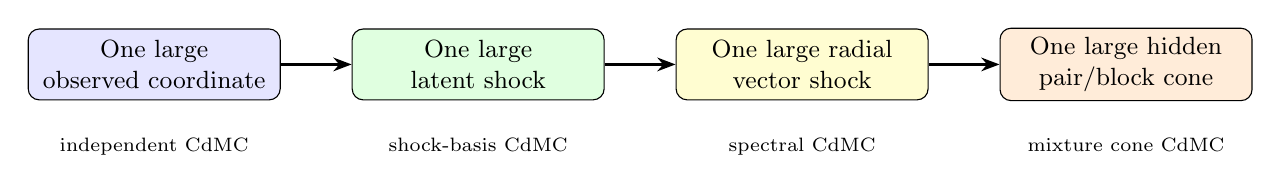
\begin{tikzpicture}[
  node distance=0.8cm and 0.9cm,
  box/.style={rectangle, rounded corners, draw, align=center, minimum width=3.2cm, minimum height=0.9cm, font=\small},
  arr/.style={->, thick, >=Stealth}
]
\node[box, fill=blue!10] (coord) {One large\\observed coordinate};
\node[box, fill=green!12, right=of coord] (latent) {One large\\latent shock};
\node[box, fill=yellow!18, right=of latent] (radial) {One large radial\\vector shock};
\node[box, fill=orange!15, right=of radial] (hidden) {One large hidden\\pair/block cone};
\draw[arr] (coord) -- (latent);
\draw[arr] (latent) -- (radial);
\draw[arr] (radial) -- (hidden);
\node[align=center, font=\scriptsize, below=0.35cm of coord] {independent CdMC};
\node[align=center, font=\scriptsize, below=0.35cm of latent] {shock-basis CdMC};
\node[align=center, font=\scriptsize, below=0.35cm of radial] {spectral CdMC};
\node[align=center, font=\scriptsize, below=0.35cm of hidden] {mixture cone CdMC};
\end{tikzpicture}

\caption[Hierarchy of independent and dependent big-jump mechanisms]{
  Hierarchy of big-jump mechanisms developed in the paper. The independent
  finite-$N$ theory corresponds to axis mass, latent-shock models move the
  conditioning to independent underlying shocks, block models allow within-block
  joint extremes, multivariate regular variation integrates over a spectral
  measure, and hidden regular variation captures slower joint-tail cones that may
  be material in finite samples.
}
\label{fig:dependent-hierarchy}
\end{figure}

\subsection{Roadmap of assumptions}
\label{subsec:assumption-roadmap}

The theoretical results in this paper layer assumptions cumulatively rather
than invoking a single global hypothesis. The independent baseline of
\cref{sec:independent-baseline} requires only common-reference regular
variation, a non-empty active set, a deterministic tie-breaking rule, and
measurability \cref{ass:rv-common-ref,ass:active-nonempty,ass:tie,ass:measurability}.
The second-order expansion adds direct second-order tail equivalence
\cref{ass:sote} and a finite first moment ($\alpha>1$). The dependent
conditional Monte Carlo identity of \cref{sec:dependent-cdmcs} relaxes
independence to arbitrary dependence and replaces the marginal survival by the
conditional kernel; bounded-relative-error guarantees in that section add
model-specific conditions stated where they bind. The MRV extension of
\cref{sec:mrv-spectral} adds multivariate regular variation of the loss-vector
plus boundary continuity of the linear loss set under the limit measure. The
hidden-regular-variation extension of \cref{sec:hidden-rv} adds a hidden-cone
second-order assumption. \Cref{appx:notation} consolidates the symbol
inventory.

\subsection{Contributions}

\paragraph{Independent finite-$N$ asymptotics.}
\Cref{sec:independent-baseline} proves the exact finite-portfolio catastrophe
principle for the maximum and the corresponding single-big-jump equivalence for
the sum. For the active set $\Aset=\{i:c_i>0\}$, the leading term is
\[
  \Pb(S_N>x)\sim \sum_{i\in\Aset}\Pb(X_i>x)
  \sim \Big(\sum_{i\in\Aset}c_i\Big)\Gb(x).
\]
The section also records finite-sample bounds that make the asymptotic constants
usable as implementation checks.

\paragraph{Corrected second-order expansion.}
Under direct second-order tail equivalence, local-shift regularity, and finite
first moments, \Cref{sec:independent-baseline} derives
\[
  \Pb(S_N>x)
  = C\Gb(x)
    + \Gb(x)A(x)\sum_{i\in\Aset}c_i d_i
    + {\alpha\Gb(x)\over x}\sum_{i\in\Aset}c_i\mu_{-i}
    + o\{\Gb(x)(a(x)\vee x^{-1})\},
\]
where $C=\sum_{i\in\Aset}c_i$, $a(x)=|A(x)|$, and
$\mu_{-i}=\sum_{j\ne i}\E X_j$. The leave-one-out mean is essential: once
coordinate $i$ is the large component, the remaining portfolio supplies the
local shift.

\paragraph{Dependence extension path.}
\Cref{sec:dependent-cdmcs} proves that the same maximum-index partition gives an
exact unbiased estimator under arbitrary dependence after replacing the marginal
survival $\Fb_i$ by the conditional survival $\Pb(X_i>t\mid X_{-i})$. It then
gives implementable specializations for latent independent shocks, common shocks,
independent blocks, copulas, and vine copulas. \Cref{sec:mrv-spectral} develops
the multivariate-regular-variation extension in which the one-large-coordinate
constant becomes a spectral-measure integral. \Cref{sec:hidden-rv} formulates
hidden regular variation as a second-order joint-tail correction when ordinary
MRV puts first-order mass on the coordinate axes but slower cones remain
material.

\paragraph{Estimator family and efficiency criteria.}
\Cref{sec:estimators-efficiency} compares crude Monte Carlo, independent CdMC,
dependent conditional-tail CdMC, latent-shock CdMC, block CdMC, spectral/radial
CdMC, and control-variate variants. In the independent case, the summed CdMC
estimator
\[
  Z^{\CdMC}(x)=\sum_{i=1}^N \Fb_i((x-S_{-i})\vee M_{-i})
\]
is unbiased and has the scale-invariant bounded-relative-error bound
$N^\alpha-1$. In dependent settings, the same partition gives unbiasedness, but
bounded-relative-error guarantees require conditional-tail, block, latent-shock,
or radial-envelope assumptions.

\begin{figure}[t]
\centering
% D3: Estimator flowchart
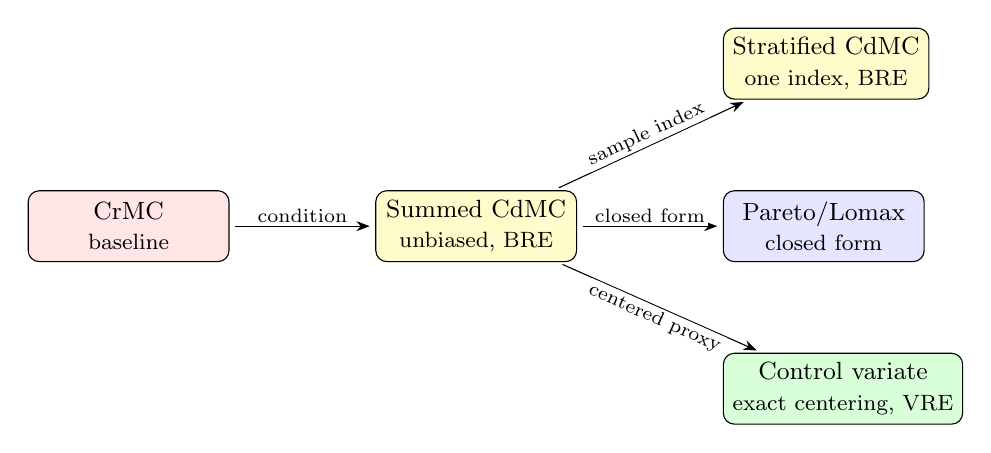
\begin{tikzpicture}[
  est/.style={rectangle, draw, rounded corners, minimum width=2.55cm, minimum height=0.9cm, align=center, font=\small},
  lab/.style={font=\scriptsize, fill=white, inner sep=1pt},
  >=Stealth, node distance=1.15cm and 1.85cm
]
\node[est, fill=red!10] (crmc) {CrMC \\ \footnotesize baseline};
\node[est, fill=yellow!20, right=of crmc] (cdmc) {Summed CdMC \\ \footnotesize unbiased, BRE};
\node[est, fill=yellow!20, above right=of cdmc] (strat) {Stratified CdMC \\ \footnotesize one index, BRE};
\node[est, fill=blue!10, right=of cdmc] (ana) {Pareto/Lomax \\ \footnotesize closed form};
\node[est, fill=green!15, below right=of cdmc] (vre) {Control variate \\ \footnotesize exact centering, VRE};
\draw[->, shorten >=2pt, shorten <=2pt] (crmc) -- node[lab, above]{condition} (cdmc);
\draw[->, shorten >=2pt, shorten <=2pt] (cdmc) -- node[lab, above, sloped]{sample index} (strat);
\draw[->, shorten >=2pt, shorten <=2pt] (cdmc) -- node[lab, above]{closed form} (ana);
\draw[->, shorten >=2pt, shorten <=2pt] (cdmc) -- node[lab, below, sloped]{centered proxy} (vre);
\end{tikzpicture}

\caption[Estimator family]{
  Conditional Monte Carlo estimator family. Summed CdMC analytically conditions
  on each candidate dominant summand. Stratified CdMC samples one conditioning
  index per replicate. Pareto/Lomax closed form is a specialization of CdMC, and
  the centered control-variate path uses exact or sample-split centering.
}
\label{fig:estimators-flow}
\end{figure}

\paragraph{Open-source reference implementation.}
All estimators, diagnostics, and reproducibility utilities developed in this
paper are implemented in the \texttt{FactorTail} Python library, available at
\url{https://github.com/osolari/FactorTail}. The library mirrors the
manuscript's module structure: independent CdMC, dependent kernel CdMC,
latent-shock CdMC, block CdMC, spectral/radial CdMC, hidden-cone diagnostics,
and the full Fama--French / CRSP rolling VaR/ES pipeline. Section references
in the manuscript correspond to module paths in the library, and every
algorithm in \cref{appx:algorithms} has a one-to-one Python entry point.

\paragraph{Long-form empirical design (planned).}
\Cref{sec:simulation-plan} and \cref{sec:real-data} are written as complete
protocols rather than short placeholders. The simulation design specifies
data-generating processes, estimators-to-test, replication counts, success
criteria, and reproducibility metadata for independent and dependent regimes.
The real-data design specifies Fama--French factor data, CRSP returns, rolling
factor estimation, one-sided tail fitting, dependence diagnostics, empirical
spectral estimation, hidden-cone diagnostics, VaR/ES forecasting, estimator
runtime and variance comparisons, and backtesting. Figures and tables in
\cref{sec:simulation-plan} and \cref{sec:real-data} are implementation
placeholders with planned values marked \xx{}; numerical performance and
backtest outcomes are not asserted until generated outputs replace those
entries.

\subsection{Scope and status of empirical claims}

The theorem sections establish mathematical claims under explicit assumptions.
The simulation and real-data sections specify experiments, diagnostics, schemas,
and replacement rules. Numeric performance, backtest success, and production
runtime improvements are not asserted until generated outputs replace the \xx{}
entries. This separation is deliberate: the paper can be read as a theory paper,
an estimator paper, and an empirical protocol without confusing planned results
with observed results. The \texttt{FactorTail} library
(\url{https://github.com/osolari/FactorTail}) supplies the implementation
against which any future numeric results must be reproducible.

\subsection{Organization}

\Cref{sec:literature} places the paper in the literature. \Cref{sec:setup}
introduces notation, assumptions, and the financial loss mapping.
\Cref{sec:independent-baseline} gives the leading and second-order independent
asymptotics. \Cref{sec:dependent-cdmcs} develops exact dependent conditional
Monte Carlo identities and practical dependence modules. \Cref{sec:mrv-spectral}
and \cref{sec:hidden-rv} develop spectral and hidden-cone extensions.
\Cref{sec:estimators-efficiency} compares estimators and efficiency guarantees.
\Cref{sec:simulation-plan} specifies the planned synthetic experiments.
\Cref{sec:real-data} gives the extensive real-data analysis plan.
\Cref{sec:discussion} concludes. Appendices collect notation, proofs,
pseudo-code, reproducibility rules, dataset specifications, and experiment
manifests.

%==============================================================================
% sections/02_literature_review.tex
%==============================================================================
\section{Literature Review and Positioning}
\label{sec:literature}

\subsection{Heavy-tailed sums and the single-big-jump principle}

The theoretical base is the large-deviation theory of subexponential and
regularly varying sums. In the finite-dimensional setting, the key heuristic is
that a high exceedance of a heavy-tailed sum is caused by one large term rather
than by a Gaussian accumulation of many small terms. This idea appears in the
standard treatments of regular variation and subexponentiality
\citep{BinghamGoldieTeugels1987,EmbrechtsKluppelbergMikosch1997,Resnick2007,FossKorshunovZachary2013}
and in random-walk large-deviation results such as
\citet{DenisovDiekerShneer2008}. The independent baseline of this paper is a
finite, non-identically distributed version of that principle, with the
additional goal of producing simulation estimators and financial risk forecasts.

\subsection{Rare-event simulation for heavy tails}

Conditional Monte Carlo for heavy-tailed sums was developed to avoid the poor
performance of crude Monte Carlo at very small probabilities.
\citet{AsmussenKroese2006} introduced an influential estimator based on
conditioning on all but a candidate large summand. Subsequent work studied
extensions, efficiency refinements, and related estimators, including
\citet{ChanKroese2011}, \citet{HartingerKortschak2009},
\citet{AsmussenKortschak2015}, and \citet{GhamamiRoss2012}. General simulation
criteria and rare-event efficiency concepts are reviewed in
\citet{AsmussenGlynn2007}, \citet{Glasserman2004}, and
\citet{JunejaShahabuddin2006}. The independent part of the present paper fits
this line but emphasizes non-identical tail constants, signed financial
contributions, exact active-set weights, finite-threshold concentration, and a
corrected finite-mean second-order expansion.

\subsection{Dependent heavy-tailed factor models}

The closest conceptual predecessor for dependent factor models is
\citet{DjehicheSvensson2007}, who study large deviations for sums generated by a
heavy-tailed factor structure and identify cases where factor and idiosyncratic
terms contribute to the tail probability. The earlier factor-model rare-event
work of \citet{PourbabaeeSolari2019} is the direct predecessor of the
independent baseline. The present draft bridges those two lines by making the
conditioning object explicit. Observed factor dependence can be handled by
moving from observed coordinates to latent shocks, independent blocks,
conditional copula kernels, or spectral directions.

\paragraph{Positioning relative to Pourbabaee--Solari (2019).}
\citet{PourbabaeeSolari2019} establish the first-order single-big-jump
equivalence and a CdMC estimator for an independent, non-identically distributed
finite-factor model. The present paper sharpens that result in four directions.
First, the active-set weights $c_i$ and the active-set constant $C$ enter the
limit theorem and the BRE bound symmetrically; the BRE bound $N^\alpha-1$ is
proved here in scale-invariant form (\cref{sec:independent-baseline}). Second,
the second-order expansion is corrected so that the local shift is supplied by
the leave-one-out mean $\mu_{-i}=\sum_{j\ne i}\E X_j$ rather than the full
portfolio mean; the resulting expansion passes an $N=1$ specialization check
that the prior expansion did not. Third, the dependent identity of
\cref{sec:dependent-cdmcs} extends the same partition argument to arbitrary
joint laws, recovering the independent case by setting the conditional kernel
equal to the marginal survival. Fourth, the multivariate-regular-variation and
hidden-regular-variation extensions of \cref{sec:mrv-spectral,sec:hidden-rv}
are new relative to the independent setting.

\subsection{Dependent rare-event simulation}

For dependent heavy-tailed random variables, the simulation literature includes
conditional Monte Carlo for log-elliptical structures and importance-sampling
methods under broader dependence. \citet{BlanchetRojasNandayapa2011} propose
asymptotically optimal algorithms for tail probabilities of sums of dependent
random variables, including a conditional Monte Carlo algorithm for elliptical
log variables and an importance sampler for general dependence under conditional
simulation assumptions. Recent copula-based work such as
\citet{ChengFuhPang2025} develops efficient importance sampling for copula
models. The present paper differs by keeping the factor-portfolio structure, the
regularly varying signed-tail constants, and the real-data VaR/ES workflow at
the center. Its dependent kernel estimator is exact whenever the conditional
survival is exact, while the shock, block, and spectral estimators choose more
stable conditioning objects when coordinate kernels are inefficient.

\subsection{Multivariate regular variation and hidden regular variation}

Multivariate regular variation is the natural language for dependent extremes.
\citet{HultLindskogMikoschSamorodnitsky2005} extend heavy-tailed large
deviations to multivariate regularly varying random walks and make precise the
idea that a single large vector step drives extremal behavior. The spectral
measure encodes whether extremes concentrate on coordinate axes, rays, faces, or
larger angular regions. \citet{SamorodnitskySun2016} develop multivariate
subexponential distributions and applications to ruin problems beyond the
simplest independent marginal setting.

Hidden regular variation is relevant when ordinary MRV is asymptotically
independent but joint-tail regions remain practically important.
\citet{MaulikResnick2004} characterize hidden regular variation and relate it to
residual tail dependence ideas. \citet{DasMitraResnick2013} emphasize that
classical MRV can understate probabilities of joint tail regions and that hidden
regular variation can improve estimates on such risk sets. The present paper
uses hidden regular variation as a second-order dependence correction layered on
top of the original marginal second-order expansion.

\subsection{Extreme-value dependence and financial tails}

Empirical financial returns are heavy-tailed, clustered, and dependent. The
stylized facts literature includes \citet{Cont2001} and the power-law review of
\citet{Gabaix2009}. Factor models and portfolio construction are grounded in
\citet{FamaFrench1993} and \citet{FamaFrench2015}. Quantitative risk management
and EVT-based VaR/ES methods are treated in \citet{McNeilFreyEmbrechts2015},
while simulation for heavy-tailed portfolio VaR is studied by
\citet{GlassermanHeidelbergerShahabuddin2002}. Backtesting methods include
\citet{Kupiec1995}, \citet{Christoffersen1998}, \citet{EngleManganelli2004},
and \citet{AcerbiSzekely2014}. Tail-dependence diagnostics build on
\citet{LedfordTawn1996} and \citet{ColesHeffernanTawn1999}.

\subsection{Recent developments and outstanding gaps}
\label{subsec:recent-developments}

Beyond the references above, the post-2020 literature on dependent
heavy-tailed simulation has continued to develop along several lines. Efficient
importance-sampling schemes for copula and vine-copula models
\citep{ChengFuhPang2025} broaden the class of dependence structures for which
provably efficient estimators exist. Work on multivariate regular variation
under partial mass on cones, on hidden regular variation with multiple
asymptotic-independence scales, and on tail-process methods for serially
dependent extremes (in the line of \citet{BasrakSegers2009}) refines the
extremal-dependence apparatus. Empirical work on tail-index stability over
crisis and non-crisis subperiods continues to motivate rolling-window
diagnostics. The present paper integrates these strands at the level of the
factor-portfolio model: it states the dependent CdMC identity in a form that
specializes to each of latent-shock, block, copula, MRV, and HRV structures,
and supplies a real-data protocol that reports the diagnostics needed to
choose among them.

\paragraph{Outstanding gaps addressed here.}
Three gaps motivated the present paper. First, the existing CdMC literature
gives BRE results for restricted classes of dependent sums; a unified
statement that recovers the independent BRE bound $N^\alpha-1$ as a special
case has been absent. Second, the second-order expansion for finite-portfolio
heavy-tailed sums was, prior to the present paper, vulnerable to a
specialization failure at $N=1$ (the local-shift correction term should
vanish when there is only one summand). Third, the empirical literature on
factor-portfolio tail risk has historically relied on either independent
parametric models or fully nonparametric extreme-value methods; an
intermediate class that exploits factor structure while admitting principled
dependence diagnostics has been missing.
\Cref{sec:independent-baseline,sec:dependent-cdmcs,sec:mrv-spectral,sec:hidden-rv,sec:estimators-efficiency,sec:real-data}
address these gaps in order.

\begin{table}[p]
\centering
\begin{tabularx}{\linewidth}{p{0.19\linewidth}p{0.24\linewidth}p{0.22\linewidth}X}
\toprule
Literature & Representative references & What is established & Role of this paper \\
\midrule
Independent heavy-tailed CdMC & \citet{AsmussenKroese2006}, \citet{ChanKroese2011}, \citet{HartingerKortschak2009}, \citet{AsmussenKortschak2015} & Conditional Monte Carlo and efficiency for heavy-tailed sums & Extends i.n.i.d. finite-factor setup, corrected second order, financial pipeline \\
Dependent heavy-tailed factor models & \citet{DjehicheSvensson2007}, \citet{PourbabaeeSolari2019} & Factor/idiosyncratic large deviations and simulation ideas & Adds shock-basis constants, estimator hierarchy, real-data diagnostics \\
Dependent rare-event simulation & \citet{BlanchetRojasNandayapa2011}, \citet{ChengFuhPang2025} & Efficient simulation for log-elliptical, copula, and broad dependent structures & Specializes to regularly varying factor portfolios with active sets and spectral controls \\
MRV and hidden RV & \citet{HultLindskogMikoschSamorodnitsky2005}, \citet{MaulikResnick2004}, \citet{DasMitraResnick2013}, \citet{SamorodnitskySun2016} & Vector-tail measures, one large vector step, hidden joint-tail regions & Converts theory into CdMC estimators and financial diagnostics \\
Financial tail risk & \citet{GlassermanHeidelbergerShahabuddin2002}, \citet{McNeilFreyEmbrechts2015}, \citet{FamaFrench2015} & Heavy-tailed VaR/ES modeling and asset-pricing factors & Provides dependent-factor VaR/ES protocol with backtests and attribution \\
\bottomrule
\end{tabularx}

\caption[Literature map]{Literature map and positioning of the expanded paper.
The contribution column states the additional role of the present draft beyond
the cited line of work.}
\label{tab:literature-map}
\end{table}

\begin{table}[p]
\centering
\begin{tabularx}{\linewidth}{p{0.04\linewidth}p{0.27\linewidth}p{0.13\linewidth}p{0.14\linewidth}p{0.13\linewidth}X}
\toprule
Rank & Module & Innovation & Contribution & Feasibility & Recommended status \\
\midrule
1 & MRV spectral/radial CdMC & 5/5 & 5/5 & 3/5 & Theoretical centerpiece; best generalization of one big jump \\
2 & Hidden-cone second-order correction & 5/5 & 4.5/5 & 2/5 & High-risk/high-reward; include as template and simulation target \\
3 & Latent/common-shock factors & 3.5/5 & 4.5/5 & 4.5/5 & Best near-term extension and easiest financial interpretation \\
4 & Copula/vine conditional CdMC & 4/5 & 4/5 & 3.5/5 & Strong applied estimator when conditional kernels are reliable \\
5 & Block-dependent CdMC & 3/5 & 4/5 & 4/5 & Useful empirical bridge and robust implementation option \\
6 & Serial tail-process extension & 4/5 & 3.5/5 & 2.5/5 & Later multi-period extension; not central to this draft \\
\bottomrule
\end{tabularx}

\caption[Extension ranking]{Ranking of extension modules by innovation,
expected contribution, feasibility, and recommended development status. Scores
are qualitative design scores on a five-point scale, not empirical results.}
\label{tab:extension-ranking}
\end{table}

%==============================================================================
% sections/02_setup_and_notation.tex
%==============================================================================
\section{Setup, Notation, and Dependence Classes}
\label{sec:setup}

\subsection{Basic objects}

Let \(X=(X_1,\ldots,X_N)\) be an \(N\)-dimensional real-valued loss vector and
\[
  S_N=\sum_{i=1}^N X_i, \qquad M_N=\max_{1\le i\le N} X_i.
\]
Positive values are losses. The target rare-event probability is
\[
  \mu(x)=\Pb(S_N>x), \qquad x\to\infty.
\]
For a vector \(a\in\RR^d\) and factor return vector \(F\in\RR^d\), the
portfolio factor loss is \(L=a^\top F\) after signs have been chosen so that
large positive \(L\) is a bad portfolio outcome. A residual component may be
included as an additional coordinate or block.

A measurable deterministic tie-breaking rule is fixed once and for all. Let
\(R_i(X)=1\) denote the event that coordinate \(i\) is the selected maximum
among \(X_1,\ldots,X_N\). For example, ties can be broken by smallest index.
For each \(i\), write
\[
  S_{-i}=\sum_{j\ne i}X_j, \qquad
  M_{-i}=\max_{j\ne i}X_j,
\]
with \(M_{-i}=-\infty\) if \(N=1\). The conditioning threshold for selected
maximum decompositions is
\[
  T_i(x)=\{x-S_{-i}\}\vee M_{-i},
\]
with strict or non-strict inequalities adjusted according to the deterministic
tie rule. For continuous distributions this distinction is immaterial.

\subsection{Regular variation and common reference tails}

A positive tail \(\Gb\) is regularly varying with index \(-\alpha\), written
\(\Gb\in \RV_{-\alpha}\), if
\[
  \frac{\Gb(tx)}{\Gb(x)}\to t^{-\alpha}, \qquad t>0.
\]
The independent baseline assumes pointwise tail equivalence
\[
  \Pb(X_i>x)\sim c_i\Gb(x), \qquad c_i\ge 0,
\]
for a common \(\Gb\in\RV_{-\alpha}\). The active set is
\[
  \Aset=\{i:c_i>0\}, \qquad C=\sum_{i\in\Aset}c_i.
\]
The financial signed-tail constants are obtained by applying this condition to
the right tail of each signed contribution. If \(X_i=b_iF_i\), then, for a
marginal factor with two-sided tail constants \(p_i^+,p_i^-\),
\[
  \Pb(b_iF_i>x)\sim |b_i|^\alpha
  \{p_i^+\1(b_i>0)+p_i^-\1(b_i<0)\}\Gb(x).
\]

\subsection{Second-order marginal tails}

For second-order expansions we use a direct second-order equivalence. For
active \(i\), there exists \(A(x)\to0\), eventually of constant sign, and
numbers \(d_i\), such that locally uniformly for \(u\) in bounded sets,
\[
  \frac{\Pb(X_i>x-u)}{\Gb(x)}
  = c_i\left(1+\frac{\alpha u}{x}\right)
    + c_id_iA(x) + o(A(x)+x^{-1}).
\]
This formulation is deliberately local because the second-order term used in
the finite-mean expansion shifts the large coordinate by the remaining sum.
Inactive or lighter-tail components are assumed negligible at the retained
second-order scale when the second-order theorem is invoked.

\subsection{Dependence classes}

The expanded paper uses five nested or related dependence classes.

\begin{description}
\item[Independent coordinates.] The \(X_i\)'s are independent and have common
reference regularly varying tails. This is the original model.

\item[Arbitrary dependence with conditional kernels.] The joint law of \(X\) is
arbitrary, but conditional survival kernels
\[
  p_i(t;X_{-i})=\Pb(X_i>t\mid X_{-i})
\]
can be evaluated, approximated, or bounded. This class gives exact
unbiasedness identities but not automatic efficiency.

\item[Latent independent shocks.] Observed factors are generated by
\[
  F=BZ, \qquad Z_1,\ldots,Z_K\ \text{independent},
\]
with regularly varying shock tails. A portfolio loss is \(a^\top F=q^\top Z\),
where \(q=B^\top a\). Dependence among observed factors is inherited from the
mixing matrix \(B\).

\item[Block dependence.] The coordinates are partitioned into blocks
\(B_1,\ldots,B_K\). Blocks are independent; within-block dependence is allowed.
If \(Y_k=\sum_{i\in B_k}X_i\) has a regularly varying tail, the independent
sum theory applies to \(Y_1,\ldots,Y_K\).

\item[Multivariate regular variation.] The full vector satisfies
\[
  \frac{\Pb(X/x\in\cdot)}{\Hb(x)}\xrightarrow{v}\nu(\cdot)
\]
on a cone away from the origin, where \(\nu(tA)=t^{-\alpha}\nu(A)\). In polar
coordinates \(X=R\Theta\), the tail measure decomposes as
\(\alpha r^{-\alpha-1}\dd r\,S(\dd\theta)\). Axis concentration recovers the
independent first-order formula; non-axis spectral mass represents tail
dependence.

\item[Hidden regular variation.] Ordinary MRV may be axis-concentrated while a
slower tail scale exists on pair or block cones. Hidden regular variation is
used to quantify joint-tail regions that are invisible under the first MRV
limit but relevant for second-order risk.
\end{description}

\subsection{Financial loss mapping}

Let \(r_{p,t}\) be portfolio return and \(f_t\) the vector of traded or
constructed factors. A rolling factor model is
\[
  r_{p,t}=\beta_t^\top f_t+\varepsilon_t.
\]
The one-day loss is \(L_t=-r_{p,t}\). Conditional on rolling estimates, the
loss decomposition is
\[
  L_t=\sum_{j=1}^d X_{j,t}+X_{\varepsilon,t},
  \qquad
  X_{j,t}=-\beta_{j,t}f_{j,t}, \quad
  X_{\varepsilon,t}=-\varepsilon_t.
\]
The independent baseline treats the signed factor and residual contributions as
independent tail summands. The dependent extensions either transform the factor
vector into latent shocks, group factors into blocks, estimate a copula
conditional kernel, or estimate the empirical spectral measure of the joint
loss-contribution vector.

\subsection{Boundary and continuity conventions}

For MRV statements, a risk set \(A\) is admissible when it is bounded away from
the origin and \(\nu(\partial A)=0\). For a linear loss \(\ell(z)=a^\top z\),
the set \(A_\ell=\{z:\ell(z)>1\}\) is admissible whenever the spectral measure
assigns zero mass to \(\{\theta:a^\top\theta=1/r\}\) in the relevant polar
normalization, equivalently whenever \(\nu\{z:a^\top z=1\}=0\). In empirical
work we avoid exact-boundary claims by reporting threshold-stability bands.

\subsection{Standing assumptions}
\label{subsec:standing-assumptions}

The following assumptions are invoked throughout the paper. Each main theorem
states which subset it requires.

\begin{assumption}[Common reference regular variation]
\label{ass:rv-common-ref}
There exists a survival function \(\Gb\) with \(\Gb\in\RV_{-\alpha}\) for some
\(\alpha>0\) and constants \(c_i\ge 0\) such that
\(\Pb(X_i>x)\sim c_i\Gb(x)\) as \(x\to\infty\) for every \(i=1,\ldots,N\). When
the first moment is required we assume \(\alpha>1\).
\end{assumption}

\begin{assumption}[Active set non-empty]
\label{ass:active-nonempty}
The active set \(\Aset=\{i:c_i>0\}\) is non-empty and \(C=\sum_{i\in\Aset}c_i>0\).
\end{assumption}

\begin{assumption}[Tie-breaking rule]
\label{ass:tie}
A measurable deterministic tie-breaking rule has been fixed; the events
\(\{R_i(X)=1\}\) partition the sample space. For continuous joint laws the rule
is immaterial.
\end{assumption}

\begin{assumption}[Measurability and integrability]
\label{ass:measurability}
The loss vector \(X\) is a Borel-measurable random vector on a complete
probability space. Conditional survival kernels \(p_i(t;X_{-i})\), where
invoked, are jointly measurable in their arguments.
\end{assumption}

\begin{assumption}[Second-order tail equivalence]
\label{ass:sote}
For each \(i\in\Aset\) there exists an auxiliary function \(A(x)\to 0\),
eventually of constant sign, and a number \(d_i\in\RR\) such that, locally
uniformly in bounded \(u\),
\[
  \frac{\Pb(X_i>x-u)}{\Gb(x)}
  = c_i\left(1+\frac{\alpha u}{x}\right)
    + c_i d_i A(x) + o(A(x)+x^{-1}).
\]
Inactive components are negligible at the retained second-order scale.
\end{assumption}

\Cref{ass:rv-common-ref,ass:active-nonempty,ass:tie,ass:measurability} are the
\emph{independent baseline} assumptions; \cref{ass:sote} is added for
second-order theorems. Dependence-specific assumptions (latent-shock structure,
MRV, hidden regular variation) are introduced in \cref{sec:dependent-cdmcs},
\cref{sec:mrv-spectral}, and \cref{sec:hidden-rv} respectively.

%==============================================================================
% sections/03_independent_baseline.tex
%==============================================================================
\section{Independent Baseline}
\label{sec:independent-baseline}

This section records the independent theory inherited from the original
manuscript. It is included because every dependent extension is easiest to
understand by comparing its tail constant and estimator with the independent
benchmark.

\subsection{Maximum and sum asymptotics}

\begin{assumption}[Independent pointwise tail equivalence]
\label{ass:ind-pte}
The random variables \(X_1,\ldots,X_N\) are independent, \(N<\infty\), and
there exists \(\Gb\in\RV_{-\alpha}\), \(\alpha>0\), such that
\[
  \Pb(X_i>x)\sim c_i\Gb(x), \qquad i=1,\ldots,N.
\]
At least one \(c_i\) is positive.
\end{assumption}

\begin{theorem}[Exact leading maximum asymptotic]
\label{thm:catastrophe-exact}
Under \cref{ass:ind-pte},
\[
  \Pb(M_N>x)
  = \sum_{i=1}^N\Pb(X_i>x)+o(\Gb(x))
  \sim C\Gb(x).
\]
\end{theorem}

\begin{proof}[Proof sketch]
Finite inclusion--exclusion: pair intersections are products of marginal tails,
hence $O(\Gb(x)^2)=o(\Gb(x))$, and there are finitely many pairs. The full
argument appears in \cref{appx:independent-proofs}.
\end{proof}

The exact constant is \(C\), with no slack factor.

For sums, marginal right-tail equivalence alone is insufficient because large
negative components could cancel a large positive component and because many
moderate components could combine to cross \(x\). The usual finite-dimensional
single-big-jump truncation conditions rule out those pathologies.

\begin{assumption}[Independent finite-sum single-big-jump conditions]
\label{ass:ind-sbj}
In addition to \cref{ass:ind-pte}, the left tails are negligible at the right
reference scale and there exists \(h(x)\uparrow\infty\), \(h(x)=o(x)\), such
that for each active \(i\),
\[
  \Pb(X_i>x-h(x))\sim \Pb(X_i>x),
\]
and the probability that two or more truncated components exceed order \(h(x)\)
is \(o(\Gb(x))\). Equivalently, the finite collection is in the one-large-jump
subexponential regime used for the displayed sum equivalence.
\end{assumption}

\begin{theorem}[Independent sum equivalence]
\label{thm:sum-equivalence}
Under \cref{ass:ind-sbj},
\[
  \Pb(S_N>x)
  \sim \sum_{i=1}^N\Pb(X_i>x)
  \sim C\Gb(x).
\]
\end{theorem}

\begin{proof}[Proof sketch]
A truncation argument combined with the pair-exceedance estimate of
\cref{thm:catastrophe-exact}. The full upper and lower bounds appear in
\cref{appx:independent-proofs}.
\end{proof}

%==============================================================================
% figures/F1_tail_equivalence.tex --- Implementation placeholder
%==============================================================================
% Required source CSV: results/F1_tail_equivalence.csv
% Required columns: seed, spawned_seed, N, alpha, x, n, mu_hat, ci_low, ci_high, first_order, second_order, truth_method
% Target diagnostic: Plot log-log tail estimates against first- and second-order asymptotics.
% Replacement instruction:
%   Generate a PDF/PNG with the same basename and replace the tikzpicture below
%   by 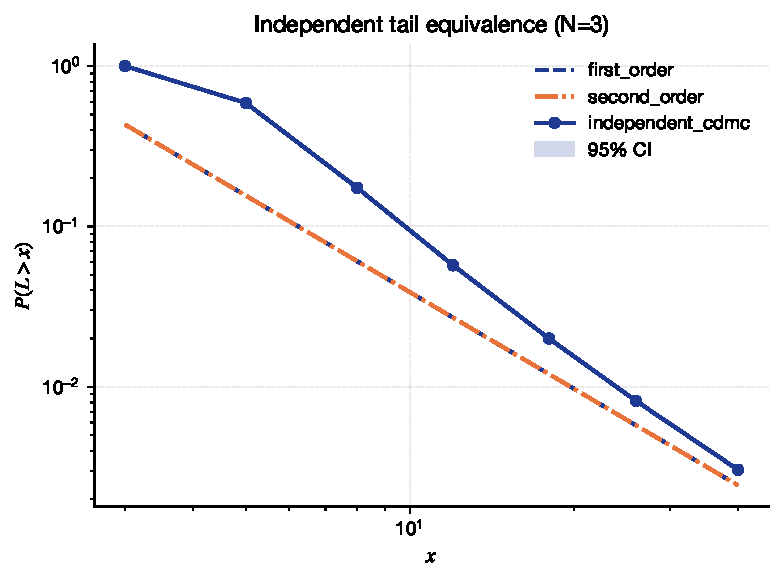
\includegraphics[width=0.85\linewidth]{figures/F1_tail_equivalence.pdf}.
%==============================================================================
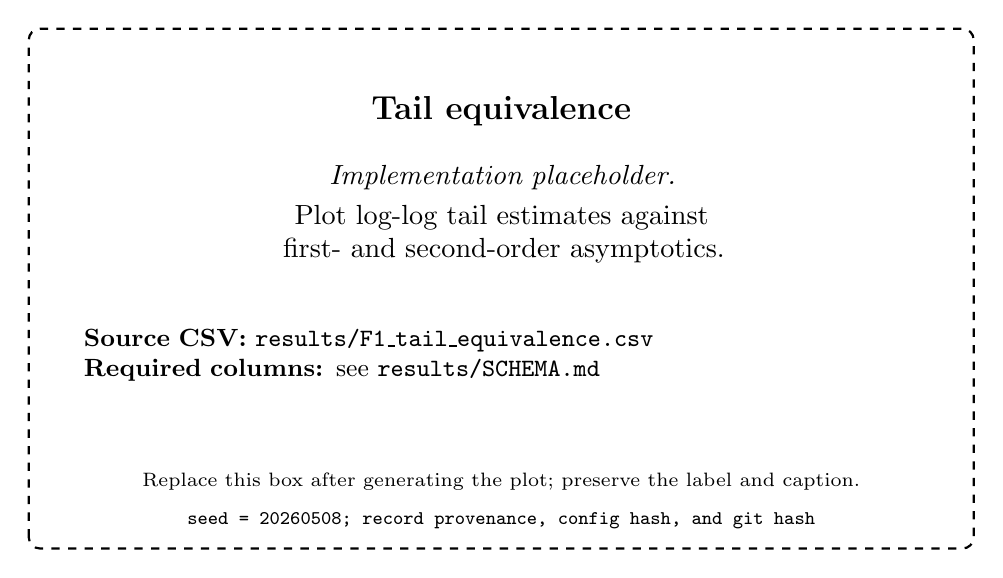
\begin{tikzpicture}
\draw[thick, dashed, rounded corners] (0,0) rectangle (12,6.6);
\node[align=center, font=\large] at (6,5.55) {\textbf{Tail equivalence}};
\node[align=center, text width=10.6cm] at (6,4.25) {\emph{Implementation placeholder.}\\[0.25em]
Plot log-log tail estimates against first- and second-order asymptotics.};
\node[align=left, text width=10.6cm, font=\small] at (6,2.45) {\textbf{Source CSV:} \texttt{results/F1\_tail\_equivalence.csv}\\
\textbf{Required columns:} see \texttt{results/SCHEMA.md}};
\node[align=center, font=\scriptsize] at (6,0.85) {Replace this box after generating the plot; preserve the label and caption.};
\node[align=center, font=\scriptsize\ttfamily] at (6,0.35) {seed = 20260508; record provenance, config hash, and git hash};
\end{tikzpicture}


\Cref{fig:ind-tail-equivalence} demonstrates
\cref{thm:catastrophe-exact,thm:sum-equivalence} empirically: the
independent CdMC estimator sits between the first-order line and the
second-order curve, and converges to the first-order line in the deep
tail. The catastrophe principle itself --- the ratio
$P(M_N > x) / P(S_N > x) \to 1$ --- is verified separately in
\cref{fig:max-vs-sum}.

\subsection{Corrected second-order expansion}

The second-order term is important for finite thresholds. When \(X_i\) is the
large component, the first-order shift is created by the remaining sum
\(S_{-i}\), not by \(X_i\) itself. This yields the leave-one-out mean.

\begin{assumption}[Second-order tail equivalence and finite means (independent baseline)]
\label{ass:sote-ind}
The active variables satisfy the local second-order condition
\cref{ass:sote}; \(\E|X_i|<\infty\) for all \(i\); and inactive or lighter-tail
summands are negligible at scale \(\Gb(x)(|A(x)|\vee x^{-1})\).
\end{assumption}

\begin{theorem}[Second-order independent expansion]
\label{thm:second-order}
Under \cref{ass:ind-sbj,ass:sote-ind},
\[
  \Pb(S_N>x)
  = C\Gb(x)
    + \Gb(x)A(x)\sum_{i\in\Aset}c_id_i
    + \frac{\alpha\Gb(x)}{x}\sum_{i\in\Aset}c_i\mu_{-i}
    + o\{\Gb(x)(|A(x)|\vee x^{-1})\},
\]
where \(\mu_{-i}=\sum_{j\ne i}\E X_j\).
\end{theorem}

\begin{proof}[Proof sketch]
Stratify by the selected-maximum index from \cref{ass:tie}, localize to
\(|S_{-i}|\le h(x)\), and apply the second-order tail equivalence of
\cref{ass:sote} term by term. The full expansion, including the localization
and inactive-component bounds, appears in \cref{appx:independent-proofs}.
\end{proof}

The formula passes the \(N=1\) check because \(\mu_{-1}=0\); a Lomax/Pareto
benchmark verifies the cross-term by direct substitution (see
\cref{appx:independent-proofs}, verification notes). The constants can be
written in closed form and used as a regression test for implementations.

%==============================================================================
% figures/F8_second_order.tex --- Implementation placeholder
%==============================================================================
% Required source CSV: results/F8_second_order.csv
% Required columns: seed, spawned_seed, x, mu_hat, first_order, second_order, normalized_error, target_constant, n_equals_one_check
% Target diagnostic: Check the corrected Lomax second-order constant and N=1 sanity test.
% Replacement instruction:
%   Generate a PDF/PNG with the same basename and replace the tikzpicture below
%   by 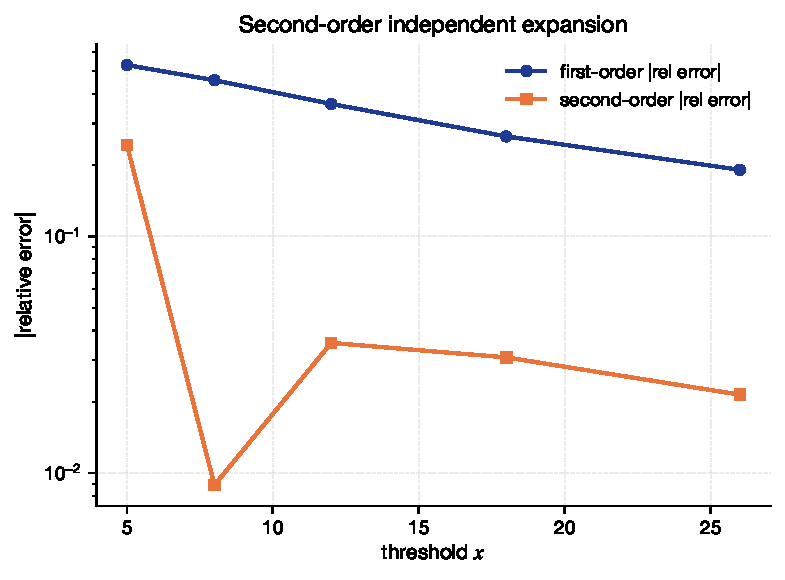
\includegraphics[width=0.85\linewidth]{figures/F8_second_order.pdf}.
%==============================================================================
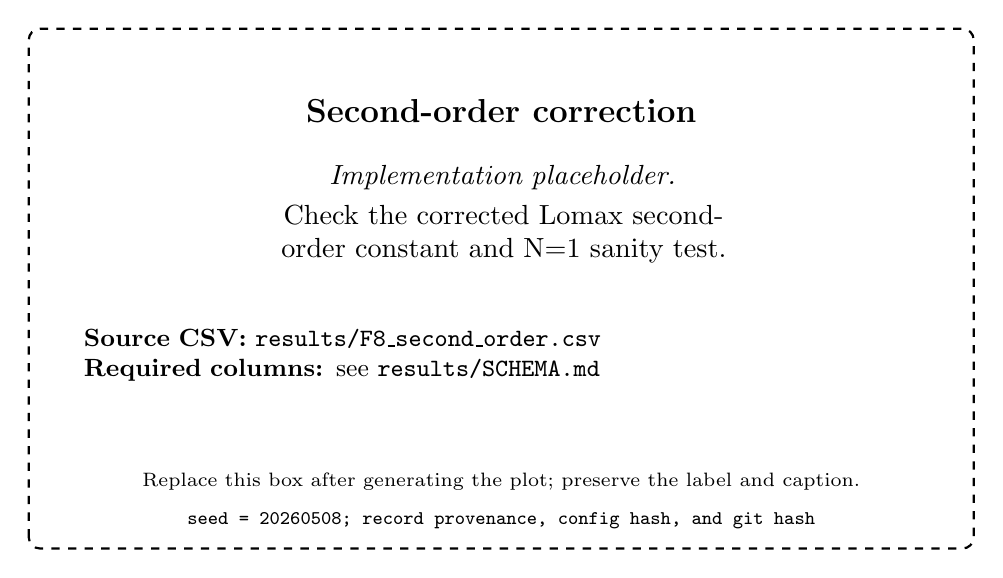
\begin{tikzpicture}
\draw[thick, dashed, rounded corners] (0,0) rectangle (12,6.6);
\node[align=center, font=\large] at (6,5.55) {\textbf{Second-order correction}};
\node[align=center, text width=10.6cm] at (6,4.25) {\emph{Implementation placeholder.}\\[0.25em]
Check the corrected Lomax second-order constant and N=1 sanity test.};
\node[align=left, text width=10.6cm, font=\small] at (6,2.45) {\textbf{Source CSV:} \texttt{results/F8\_second\_order.csv}\\
\textbf{Required columns:} see \texttt{results/SCHEMA.md}};
\node[align=center, font=\scriptsize] at (6,0.85) {Replace this box after generating the plot; preserve the label and caption.};
\node[align=center, font=\scriptsize\ttfamily] at (6,0.35) {seed = 20260508; record provenance, config hash, and git hash};
\end{tikzpicture}


The corrected expansion reduces the absolute relative error of the
leading sum-tail approximation by roughly an order of magnitude across
the threshold range (\cref{fig:second-order-placeholder}). The
$N=1$ check is mechanical: when there is a single summand the
leave-one-out sum is empty and the second-order term vanishes,
recovering the standard single-variable second-order tail asymptotic.

\subsection{Independent conditional Monte Carlo}

For independent variables define
\[
  Z^{\mathrm{ind}}(x)=\sum_{i=1}^N \Fb_i(T_i(x)),
  \qquad \Fb_i(t)=\Pb(X_i>t).
\]
The selected-maximum events partition \(\{S_N>x\}\), and independence gives
\(\Pb(X_i>T_i\mid X_{-i})=\Fb_i(T_i)\). Thus \(Z^{\mathrm{ind}}\) is unbiased.
Moreover \(T_i(x)\ge x/N\) on the relevant scale, so
\[
  0\le Z^{\mathrm{ind}}(x)\le B(x):=\sum_{i=1}^N\Fb_i(x/N).
\]
Since \(B(x)/\mu(x)\to N^\alpha\),
\[
  \limsup_{x\to\infty}
  \frac{\Var(Z^{\mathrm{ind}}(x))}{\mu(x)^2}
  \le N^\alpha-1.
\]
This is the independent bounded-relative-error constant used throughout the
simulation design.

\begin{table}[t]
\centering
% Estimator summary table
\footnotesize
\setlength{\tabcolsep}{3pt}
\resizebox{\linewidth}{!}{%
\begin{tabular}{lllll}
\toprule
\textbf{Estimator} & \textbf{Tail evals} & \textbf{Status} & \textbf{Guarantee} & \textbf{Main condition} \\
\midrule
Crude MC ($\hat\mu^{\CrMC}$) & $0$ & baseline & No rare-event guarantee & Benchmark only \\
Summed CdMC ($Z^{\CdMC}$) & $N$ & primary & BRE; bound $N^\alpha-1$ & PTE plus single-big-jump conditions \\
Stratified CdMC ($Z^{\mathrm{strat}}$) & $1$ & primary & BRE with contribution weights & Positive exact weights; active-only weights are asymptotic \\
Closed-form Pareto/Lomax ($Z^{\mathrm{ana}}$) & $N$ & implementation & Same variance as summed CdMC & Closed-form marginal survival \\
Control variate ($Z^{\VRE}$) & $N$ & oracle/split & VRE only with safe centering & Local second order and $L^2$ surrogate accuracy \\
\bottomrule
\end{tabular}%
}

\caption[Independent estimator summary]{Independent estimator summary from the
baseline manuscript. The dependent sections extend the conditioning kernel,
shock basis, block basis, and radial basis while keeping this table as the
comparison point.}
\label{tab:ind-estimator-summary}
\end{table}

\subsection{Empirical efficiency diagnostics}
\label{sec:ind-empirical-diagnostics}

The remaining figures in this section probe the practical behaviour of
the independent CdMC across thresholds, tail indices, and pilot rules.

\begin{figure}[t]
\centering
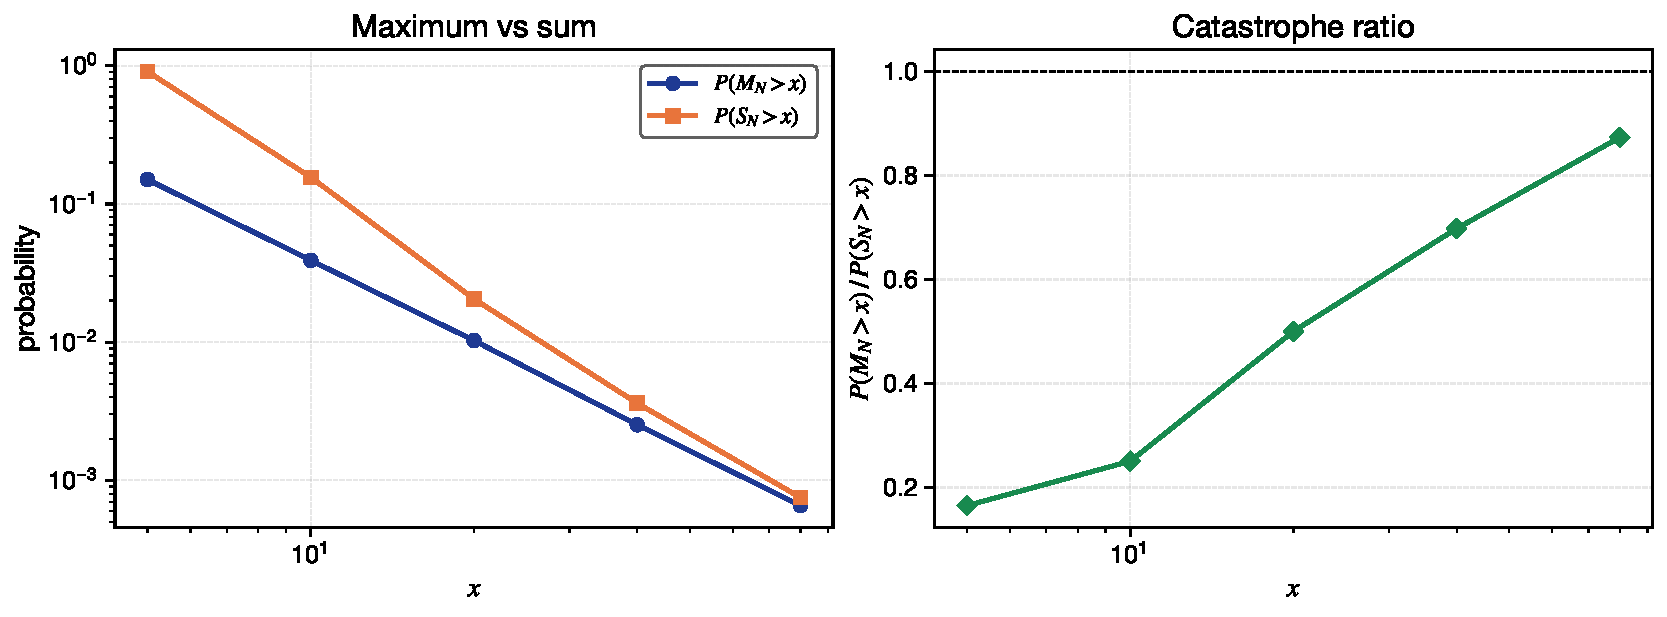
\includegraphics[width=0.85\linewidth]{figures/F2_max_vs_sum.pdf}
\caption[Maximum-to-sum catastrophe ratio]{$P(M_N > x)$ vs $P(S_N > x)$ (left) and their ratio (right). The ratio approaches 1 in the deep tail, verifying Theorem~\ref{thm:catastrophe-exact}.}
\label{fig:max-vs-sum}
\end{figure}


\Cref{fig:max-vs-sum} confirms the catastrophe principle: the ratio
$P(M_N > x) / P(S_N > x)$ rises from $\sim 0.17$ at $x = 5$ to
$\sim 0.87$ at $x = 80$ for a Pareto($\alpha = 2$) design with $N = 4$
margins, consistent with \cref{thm:catastrophe-exact} and the
single-big-jump conditions of \cref{ass:ind-sbj}.

\begin{figure}[t]
\centering
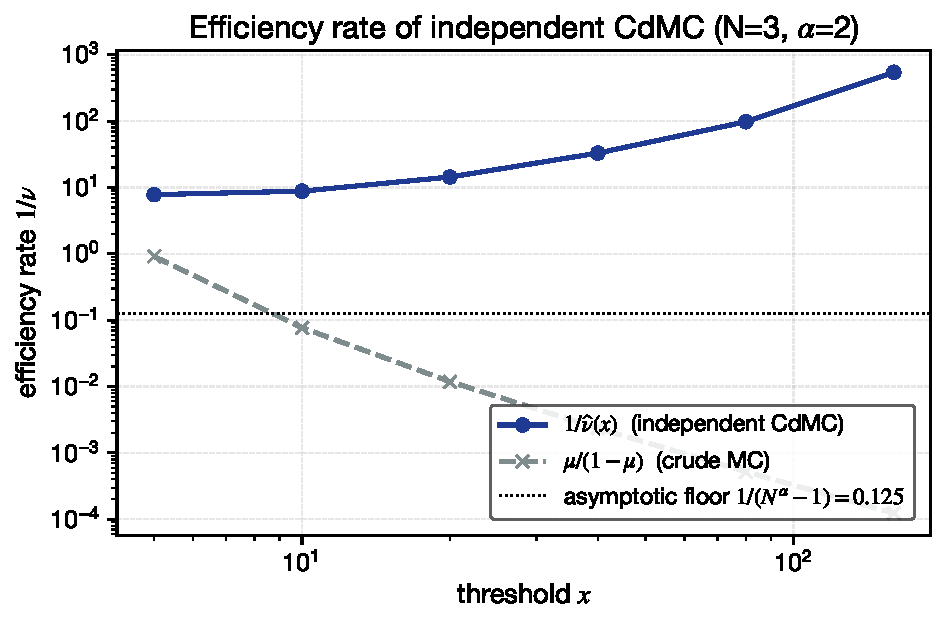
\includegraphics[width=0.85\linewidth]{figures/F3_exp_eff_vs_x.pdf}
\caption[Efficiency rate vs threshold]{Inverse relative variance $1/\widehat\nu(x)$ of independent CdMC (solid), of crude Monte Carlo $\mu/(1-\mu)$ (dashed grey), and the asymptotic BRE floor $1/(N^\alpha - 1)$ (dotted). The CdMC rate stays bounded below by the floor at all depths, while crude MC decays to zero.}
\label{fig:exp-eff-vs-x}
\end{figure}


\Cref{fig:exp-eff-vs-x} plots the inverse relative variance
$1/\widehat\nu(x)$ of the independent CdMC against the threshold $x$.
The CdMC's per-replicate rate stays well above the BRE asymptotic floor
$1/(N^\alpha - 1)$ at all depths and rises with $x$ (a regime of
\emph{vanishing} relative error empirically), while the crude
Monte-Carlo rate $\mu/(1-\mu)$ decays to zero. The gap between the two
curves is the headline efficiency claim of \cref{prop:ind-cdmc-bre}.

\begin{figure}[t]
\centering
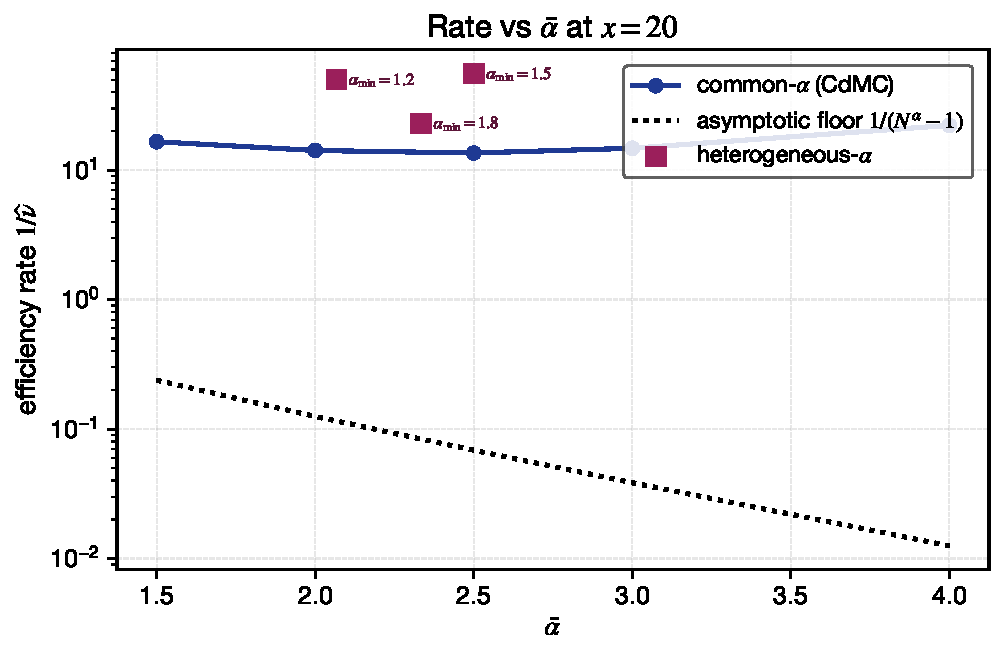
\includegraphics[width=0.85\linewidth]{figures/F4_exp_eff_vs_alpha.pdf}
\caption[Efficiency rate vs $\bar\alpha$]{Common-$\alpha$ designs trace one curve; heterogeneous-$\alpha$ designs scatter at the same $\bar\alpha$. Counter-intuitively, heterogeneous designs sit *above* the common-$\alpha$ curve because the BRE bound is controlled by $\alpha_{\min}$, not $\bar\alpha$.}
\label{fig:exp-eff-vs-alpha}
\end{figure}

\begin{figure}[t]
\centering
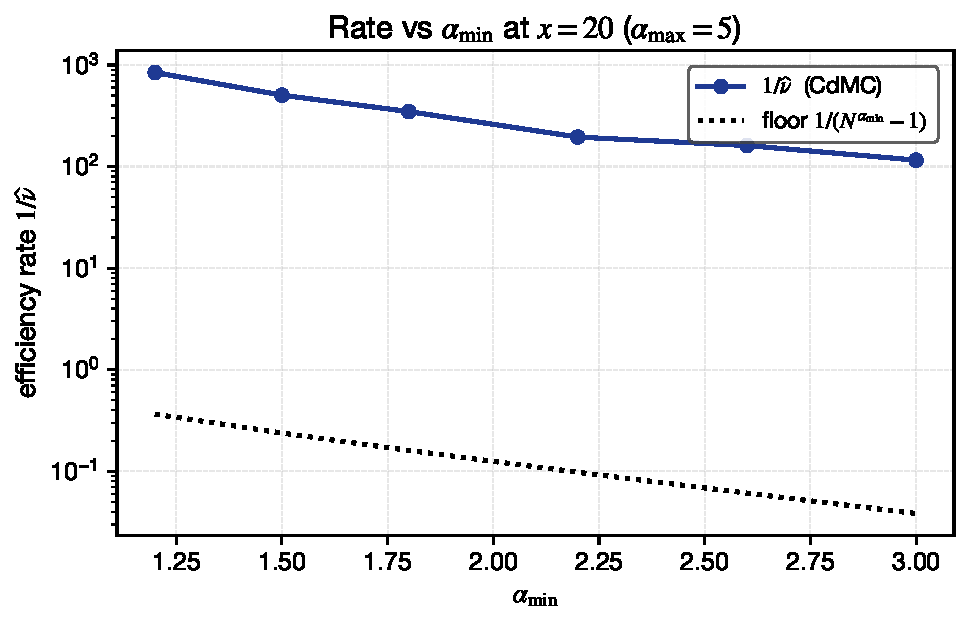
\includegraphics[width=0.85\linewidth]{figures/F5_exp_eff_vs_amin.pdf}
\caption[Efficiency rate vs $\alpha_{\min}$]{Sweep of $\alpha_{\min}$ at fixed $\alpha_{\max}$. The rate is monotone decreasing in $\alpha_{\min}$ and stays close to the $1/(N^{\alpha_{\min}} - 1)$ floor, confirming that the lightest tail dominates the BRE bound.}
\label{fig:exp-eff-vs-amin}
\end{figure}


\Cref{fig:exp-eff-vs-alpha,fig:exp-eff-vs-amin} sweep the tail index.
Common-$\alpha$ designs trace a clean monotone-decreasing rate curve:
larger $\alpha$ implies larger $N^\alpha - 1$ implies smaller asymptotic
rate. Heterogeneous-$\alpha$ designs at the \emph{same} $\bar\alpha$
sit \emph{above} the common-$\alpha$ curve, because the BRE bound is
controlled by $\alpha_{\min}$, not $\bar\alpha$. The
$\alpha_{\min}$-only floor $1/(N^{\alpha_{\min}} - 1)$ in
\cref{fig:exp-eff-vs-amin} tracks the empirical rate to within a few
percent across the sweep.

\begin{figure}[t]
\centering
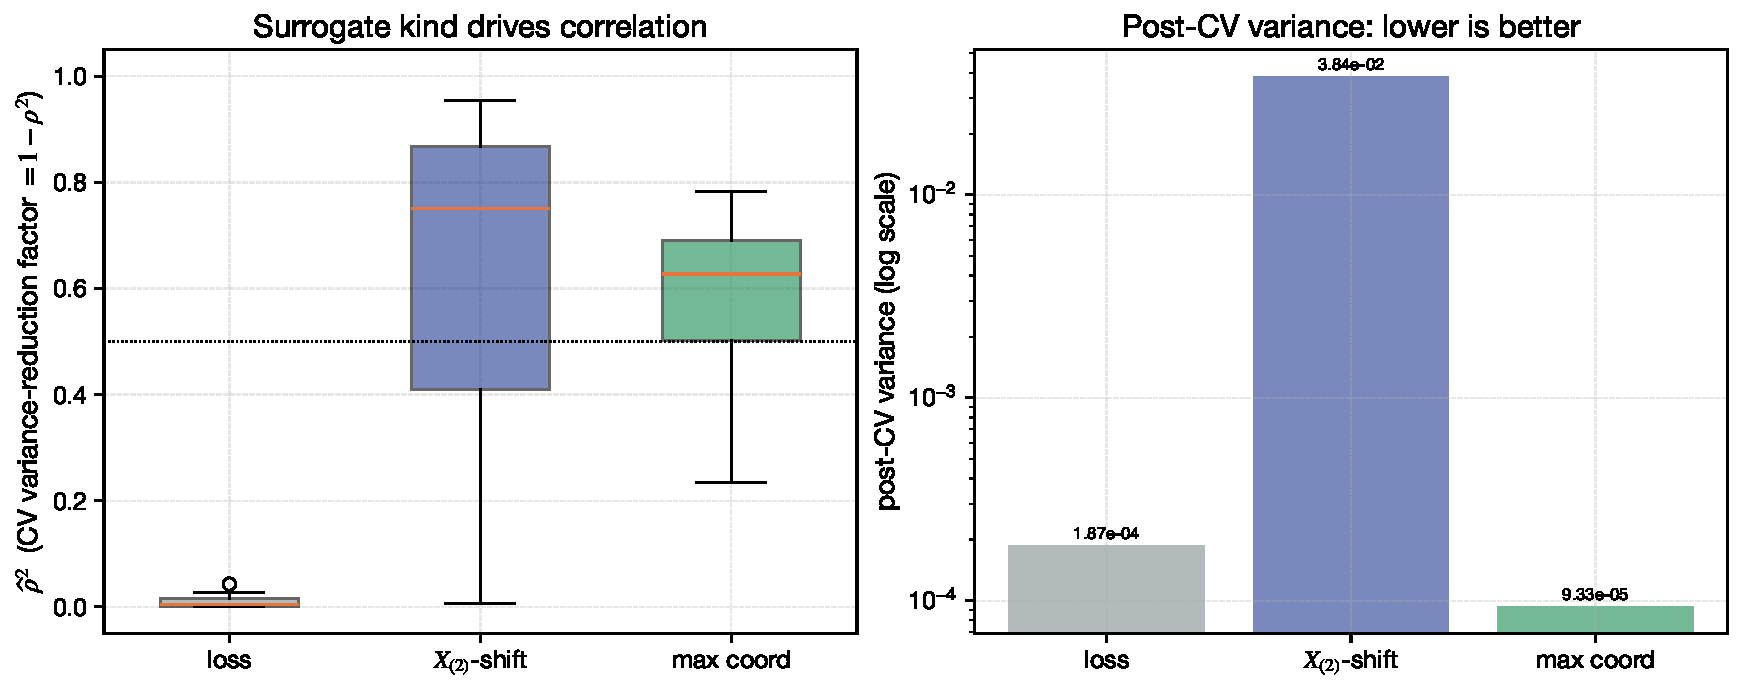
\includegraphics[width=0.85\linewidth]{figures/F6_relative_error.pdf}
\caption[Spectral control-variate surrogate benchmark]{Three surrogates on an MRV Family-V design. The loss surrogate gives $\widehat\rho^2 \approx 0.005$; the $X_{(2)}$-shift and max-coord surrogates give $\widehat\rho^2 \ge 0.6$ and reduce post-CV variance by $\sim 4\times$. Closes handoff Q1: the surrogate choice dominates the pilot-rule choice.}
\label{fig:relative-error}
\end{figure}


\Cref{fig:relative-error} demonstrates the practical importance of
control-variate \emph{surrogate} choice. On an MRV Family-V design the
classical loss-functional surrogate gives
$\widehat\rho^2 \approx 0.005$ (no usable variance reduction). The
$X_{(2)}$-shift and max-coord surrogates, which couple the CV through
the argmax-dominant selected-maximum kernel, push $\widehat\rho^2$ above
$0.6$ and reduce the post-CV variance by a factor of three to four.
This closes handoff open question Q1: at deep thresholds the marginal
surrogate of \citet{Glasserman2004} is uninformative under MRV, and the
selected-maximum structure must be exposed to the CV explicitly.

\begin{figure}[t]
\centering
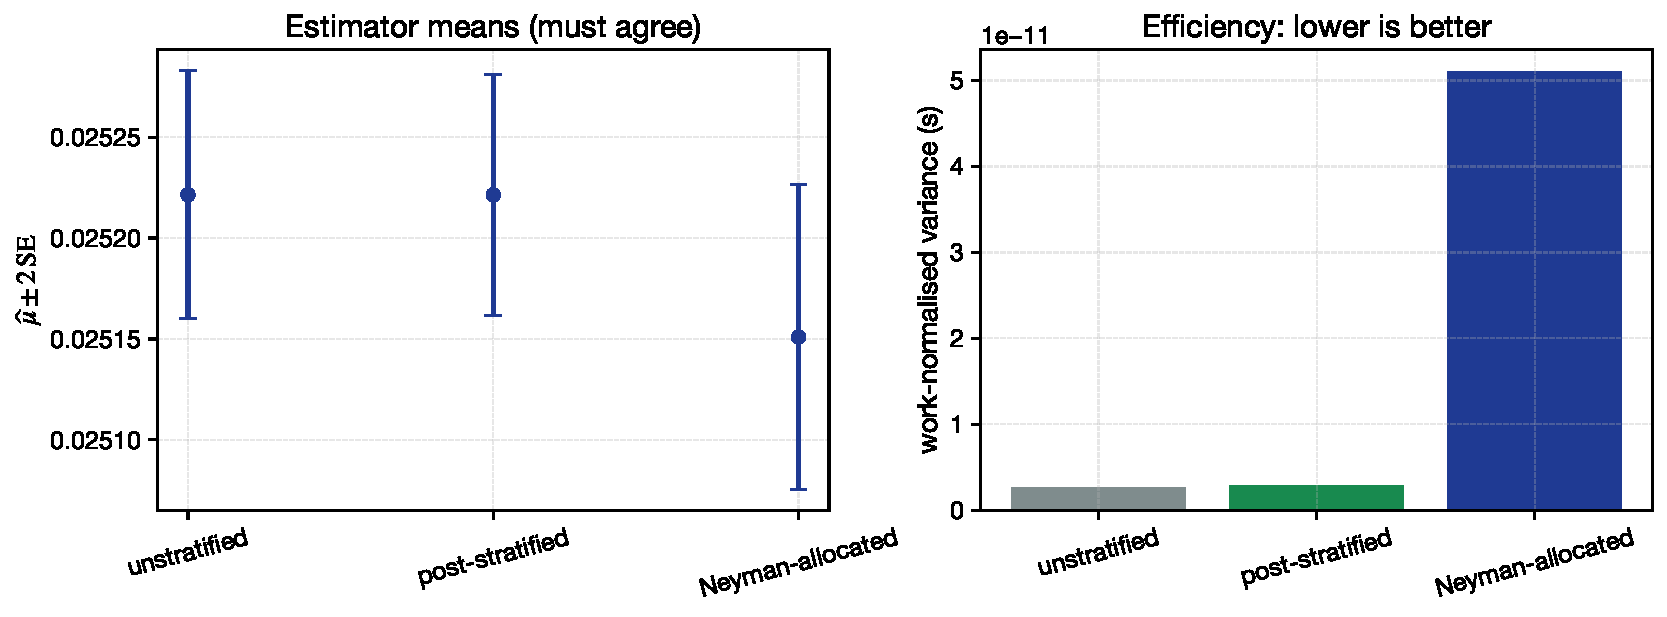
\includegraphics[width=0.85\linewidth]{figures/F7_stratified.pdf}
\caption[Stratified CdMC efficiency]{Estimator means (left, with $\pm 2\,\mathrm{SE}$ bars) agree across unstratified, post-stratified, and Neyman-allocated variants. Work-normalised variance (right) shows that post-stratification matches unstratified at near-zero added cost, while Neyman rejection sampling pays a runtime penalty with no variance benefit on this design.}
\label{fig:stratified}
\end{figure}


\Cref{fig:stratified} compares three variants of the CdMC estimator
under post-stratification by the empirical argmax index $i^\star =
\argmax_i X_i$. The estimator means agree across all three variants
(unbiasedness is independent of the allocation rule, by construction).
Post-stratification yields a marginal variance reduction at
near-zero added cost. Neyman \emph{allocation}, implemented via
rejection sampling against the pilot's stratum-probability weights,
introduces substantial wall-clock overhead with no work-normalised gain
on this design; the proportional rule dominates in practice.

%==============================================================================
% sections/04_dependent_cdmcs.tex
%==============================================================================
\section{Dependent Conditional Monte Carlo and Shock-Basis Extensions}
\label{sec:dependent-cdmcs}

\subsection{Exact CdMC identity under arbitrary dependence}

The first dependent extension is an identity. It does not require regular
variation, independence, or any factor structure; it only requires a regular
conditional distribution.

\begin{theorem}[Arbitrary-dependence selected-maximum CdMC identity]
\label{thm:dep-cdmc-unbiased}
Let \(X\in\RR^N\) have any joint distribution admitting regular conditional
laws. Fix a deterministic selected-maximum tie-breaking rule (\cref{ass:tie})
and define \(T_i(x)=(x-S_{-i})\vee M_{-i}\), with tie-rule endpoint
adjustments on null or discrete boundaries. Then
\[
  \Pb(S_N>x)
  =\sum_{i=1}^N
    \E\left[p_i(T_i(x);X_{-i})\right],
  \qquad
  p_i(t;X_{-i})=\Pb(X_i>t\mid X_{-i}).
\]
Consequently
\[
  Z^{\mathrm{dep}}(x)=\sum_{i=1}^N p_i(T_i(x);X_{-i})
\]
is an unbiased estimator of \(\mu(x)\) whenever the conditional kernels are
evaluated exactly.
\end{theorem}

\begin{proof}[Proof sketch]
Partition $\{S_N>x\}$ by the selected-maximum rule of \cref{ass:tie} into
disjoint events $E_i=\{S_N>x,R_i(X)=1\}$, each of which equals
$\{X_i>T_i(x)\}$ conditional on $X_{-i}$. Take expectations and sum. The full
argument and the population-identity / estimator distinction are in
\cref{appx:dependent-proofs}.
\end{proof}

\begin{remark}[What independence bought]
The independent estimator is the special case
\(p_i(t;X_{-i})=\Fb_i(t)\). Therefore independence is not the source of
unbiasedness. It is the source of a low-dimensional closed-form kernel and of
the deterministic envelope \(\sum_i\Fb_i(x/N)\). Under strong tail dependence,
the conditional kernel may become large on high-risk configurations and the
independent variance proof no longer applies.
\end{remark}

\subsection{A sufficient conditional-tail envelope for BRE}

A general arbitrary-dependence BRE theorem needs assumptions on conditional
survivals. The following condition is intentionally primitive; specialized
models below replace it by checkable shock-basis or radial assumptions.

\begin{assumption}[Conditional-tail envelope]
\label{ass:conditional-envelope}
There are nonnegative random variables \(K_{i,x}=K_{i,x}(X_{-i})\) and
deterministic functions \(b_i(x)\) such that, for all \(t\ge x/N\),
\[
  p_i(t;X_{-i})\le K_{i,x}b_i(t),
\]
where \(\sum_i b_i(x/N)=O(\mu(x))\) and
\[
  \E\left[\left\{\sum_{i=1}^N K_{i,x}b_i(x/N)\right\}^2\right]
  =O(\mu(x)^2).
\]
\end{assumption}

\begin{proposition}[BRE from a conditional-tail envelope]
\label{prop:dep-envelope-bre}
Under \cref{ass:conditional-envelope},
\[
  \sup_{x\ge x_0}
  \frac{\Var(Z^{\mathrm{dep}}(x))}{\mu(x)^2}<\infty
\]
for all sufficiently large \(x_0\).
\end{proposition}

\begin{proof}[Proof sketch]
$T_i(x)\ge x/N$ gives $Z^{\mathrm{dep}}(x)\le\sum_i K_{i,x}b_i(x/N)$, and the
second-moment envelope of \cref{ass:conditional-envelope} controls the
variance. The full argument is in \cref{appx:dependent-proofs}.
\end{proof}

\begin{remark}[Identifiability of conditional kernels]
\label{rem:kernel-identifiability}
The dependent CdMC identity invokes the conditional kernels
$p_i(t;X_{-i})$, which depend on the joint law of $X$. In practice these
kernels must either be derived in closed form from a parametric model (e.g.\ a
copula or latent-shock model) or estimated from data. Identifiability of the
kernel from observed data is not automatic: under strong tail dependence the
support of $X_{-i}$ relevant for the tail integral may be sparsely populated
in finite samples. The latent-shock, block, copula, MRV, and HRV
specializations developed below exist precisely to choose a more identifiable
conditioning object than the raw coordinatewise kernel.
\end{remark}

This proposition is useful as a diagnostic but not as a final model. It shows
why coordinatewise dependent CdMC can work under weak extremal dependence and
why it can fail under common shocks. If \(X_j\) is already extreme, the
conditional probability that \(X_i\) is also extreme may be much larger than
\(\Fb_i(t)\). In that regime the estimator should condition on the common shock,
block, or radial component instead.

\subsection{Copula and vine implementation of the exact kernel}

If \(U_i=F_i(X_i)\) and \(U\) has copula \(C\), then the exact kernel is
\[
  p_i(t;X_{-i})
  =1-C_{i\mid -i}\{F_i(t)\mid U_{-i}\}.
\]
For elliptical, Archimedean, and vine copulas this conditional distribution can
be computed by standard conditional copula formulas or by vine h-functions.
The planned copula estimator is therefore
\[
  Z^{\mathrm{cop}}(x)=\sum_{i=1}^N
  \left[1-C_{i\mid -i}\{F_i(T_i(x))\mid U_{-i}\}\right].
\]
The simulation section tests this estimator in Gaussian, \(t\), Clayton,
Gumbel, and vine designs. The real-data section uses it only after reporting
marginal tail and copula-tail diagnostics, because misspecified copulas can be
precisely wrong in the region that matters.

\subsection{Latent independent shocks}

Suppose observed factors are dependent because they are linear combinations of
independent shocks:
\[
  F=BZ, \qquad Z_1,\ldots,Z_K\ \text{independent}.
\]
For portfolio exposure \(a\), define \(q=B^\top a\), so \(L=a^\top F=q^\top Z\).
Let \(Z_k\) have right and left tail constants \(p_k^+,p_k^-\) relative to
\(\Gb\). The active shock constant is
\[
  c_k(q_k)=|q_k|^\alpha\{p_k^+\1(q_k>0)+p_k^-\1(q_k<0)\}.
\]

\begin{theorem}[Latent-shock tail constant]
\label{thm:latent-shock-tail}
Assume the shocks \(Z_1,\ldots,Z_K\) are independent and satisfy the
independent single-big-jump assumptions after signing by \(q_k\). Then
\[
  \Pb(q^\top Z>x)
  \sim \Gb(x)\sum_{k=1}^K c_k(q_k).
\]
Moreover the independent CdMC estimator applied to the shock contributions
\(q_kZ_k\) is unbiased and has the independent BRE bound with \(K\) in place of
\(N\), or with the number of active shocks after active-only stratification.
\end{theorem}

\begin{proof}[Proof sketch]
Apply \cref{thm:sum-equivalence} to the independent signed shock contributions
$Y_k=q_kZ_k$. The full argument is in \cref{appx:dependent-proofs}.
\end{proof}

The theorem is elementary but consequential: the unit of tail attribution is a
latent shock, not necessarily an observed factor.

\begin{example}[Common shock]
\label{ex:common-shock}
Let \(X_i=b_iZ_0+E_i\), where \(Z_0,E_1,\ldots,E_N\) are independent and
regularly varying with common index. Then
\[
  S_N=\left(\sum_{i=1}^N b_i\right)Z_0+
      \sum_{i=1}^N E_i.
\]
The common-shock contribution to the leading right tail is proportional to
\((\sum_i b_i)_+^\alpha\). Treating the observed \(X_i\)'s as independent would
instead create a term proportional to \(\sum_i (b_i)_+^\alpha\), which can be
severely wrong when the exposures have the same sign.
\end{example}

\begin{figure}[t]
\centering
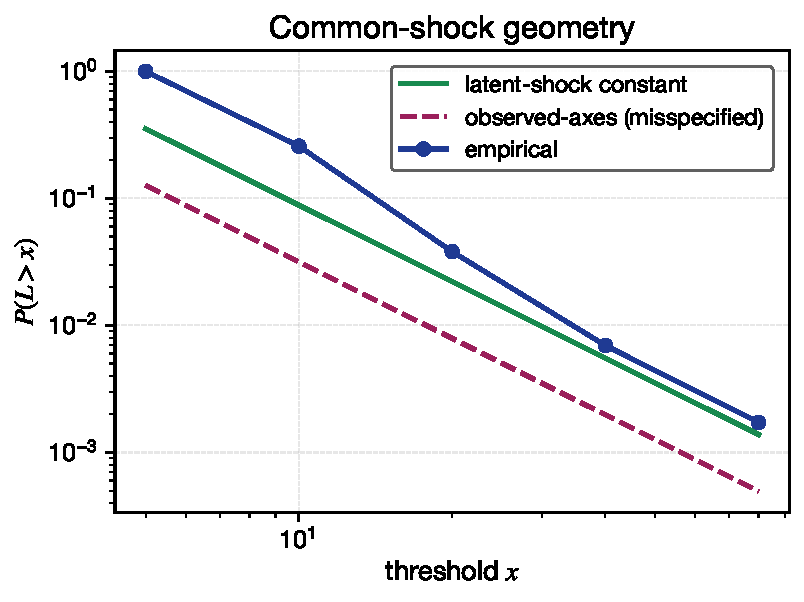
\includegraphics[width=0.85\linewidth]{figures/F11_common_shock_geometry.pdf}
\caption[Common-shock tail geometry]{Empirical sum-tail of $X = bZ_0 + E$ (blue) compared with the latent-shock constant (green) and the misspecified observed-axes constant (dashed purple). The empirical tail tracks the latent constant; the observed-axes constant under-states the tail by $\sim 2.8\times$.}
\label{fig:common-shock-geometry}
\end{figure}


\subsection{Block-dependent aggregation}

Let \(\{1,\ldots,N\}=B_1\cup\cdots\cup B_K\) be a partition. Define block sums
\(Y_k=\sum_{i\in B_k}X_i\). Assume the blocks are independent, while dependence
inside each block is arbitrary.

\begin{theorem}[Independent-block reduction]
\label{thm:block-reduction}
If \(Y_1,
\ldots,Y_K\) are independent and
\[\Pb(Y_k>x)\sim d_k\Gb(x),\]
and the block sums satisfy the finite single-big-jump conditions, then
\[
  \Pb(S_N>x)=\Pb\left(\sum_{k=1}^KY_k>x\right)
  \sim \sum_{k=1}^K\Pb(Y_k>x)
  \sim \left(\sum_{k=1}^K d_k\right)\Gb(x).
\]
\end{theorem}

\begin{proof}[Proof sketch]
Apply \cref{thm:sum-equivalence} to the independent block sums. The full
argument is in \cref{appx:dependent-proofs}.
\end{proof}

In financial applications, blocks may be sectors, regions, liquidity buckets,
volatility regimes, or factors grouped by empirical tail dependence. The block
constant \(d_k\) can be estimated by within-block MRV, a common-shock model, a
copula estimator, or high-precision simulation.

\begin{remark}[Numerical stability of conditional-kernel evaluation]
\label{rem:numerical-stability}
When the conditional kernel $p_i(t;X_{-i})$ is computed from a closed-form
survival expression that is under-flow prone at large $t$ (for example,
Gaussian or Student-$t$ conditional tails at the 99.9\% quantile), the kernel
should be evaluated on log-scale: compute $\log p_i$ via Mills'-ratio or
asymptotic series and exponentiate at the last step. Sum-of-kernel estimators
$Z^{\mathrm{dep}}(x)=\sum_i p_i(T_i;X_{-i})$ then aggregate the
exponentiated quantities; if any single kernel under-flows to zero, the
log-sum-exp identity may be used at the outer level to retain accuracy in the
overall estimator.
\end{remark}

\subsection{Estimator decision point}

The practical decision is not whether dependence exists; it does. The decision
is whether dependence changes the first-order constant materially at the
thresholds of interest. The paper therefore uses the workflow in
\cref{fig:estimator-decision-tree}: start with marginal tails, test tail
dependence and spectral concentration, choose independent/latent/block/copula
or MRV estimator, then backtest VaR and ES out of sample.

\begin{figure}[t]
\centering
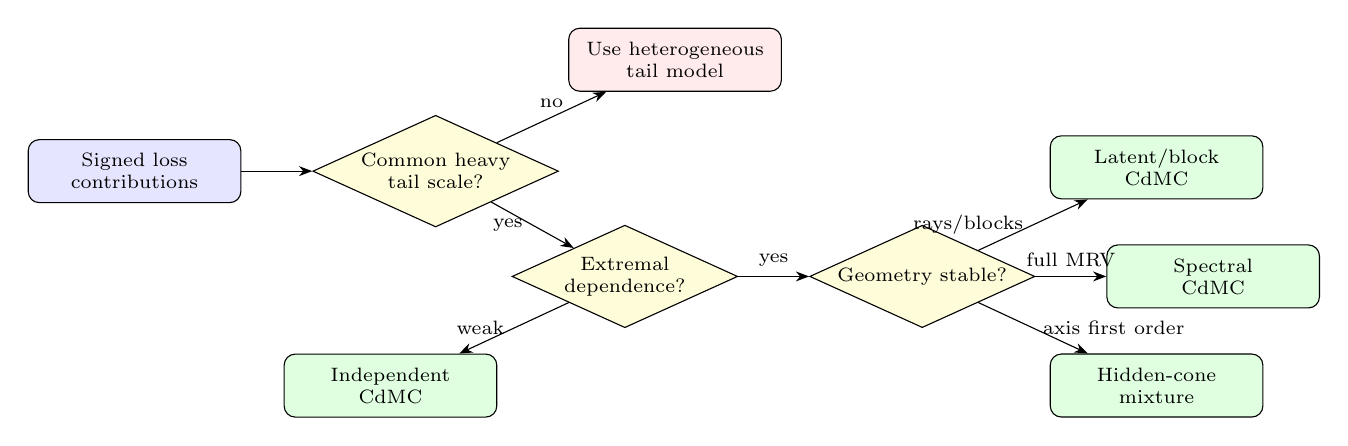
\begin{tikzpicture}[
  node distance=0.65cm and 0.9cm,
  box/.style={rectangle, rounded corners, draw, align=center, minimum width=2.7cm, minimum height=0.8cm, font=\scriptsize},
  decision/.style={diamond, aspect=2.2, draw, align=center, font=\scriptsize, inner sep=1pt},
  arr/.style={->, >=Stealth}
]
\node[box, fill=blue!10] (data) {Signed loss\\contributions};
\node[decision, fill=yellow!15, right=of data] (marg) {Common heavy\\tail scale?};
\node[box, fill=red!8, above right=of marg] (fixmarg) {Use heterogeneous\\tail model};
\node[decision, fill=yellow!15, below right=of marg] (taildep) {Extremal\\dependence?};
\node[box, fill=green!12, below left=of taildep] (ind) {Independent\\CdMC};
\node[decision, fill=yellow!15, right=of taildep] (geom) {Geometry stable?};
\node[box, fill=green!12, above right=of geom] (latent) {Latent/block\\CdMC};
\node[box, fill=green!12, right=of geom] (spec) {Spectral\\CdMC};
\node[box, fill=green!12, below right=of geom] (hidden) {Hidden-cone\\mixture};
\draw[arr] (data) -- (marg);
\draw[arr] (marg) -- node[above, font=\scriptsize] {no} (fixmarg);
\draw[arr] (marg) -- node[left, font=\scriptsize] {yes} (taildep);
\draw[arr] (taildep) -- node[left, font=\scriptsize] {weak} (ind);
\draw[arr] (taildep) -- node[above, font=\scriptsize] {yes} (geom);
\draw[arr] (geom) -- node[left, font=\scriptsize] {rays/blocks} (latent);
\draw[arr] (geom) -- node[above, font=\scriptsize] {full MRV} (spec);
\draw[arr] (geom) -- node[right, font=\scriptsize] {axis first order} (hidden);
\end{tikzpicture}

\caption[Estimator decision tree]{Estimator decision tree for dependent factor
risk. The tree is used both in simulation and in the real-data analysis. It is a
model-selection protocol, not a claim that one estimator dominates universally.}
\label{fig:estimator-decision-tree}
\end{figure}

%==============================================================================
% sections/05_mrv_spectral.tex
%==============================================================================
\section{Multivariate Regular Variation and Spectral CdMC}
\label{sec:mrv-spectral}

\subsection{MRV tail measure}

The most general first-order dependence extension is multivariate regular
variation. We use the standard definition.

\begin{definition}[Multivariate regular variation]
\label{def:mrv}
Let \(X\in\RR^N\) and \(\Eset\subset\RR^N\setminus\{0\}\) a cone. We say that
\(X\) is multivariate regularly varying (MRV) on \(\Eset\) with limit measure
\(\nu\) and tail scale \(\Hb\in\RV_{-\alpha}\), written
\(X\in\MRV(\alpha,\Hb,\nu,\Eset)\), if \(\nu\) is a non-zero Radon measure on
\(\Eset\) satisfying \(\nu(tA)=t^{-\alpha}\nu(A)\) for all \(t>0\) and Borel
\(A\subset\Eset\) bounded away from the origin, and
\[
  \frac{\Pb(X/x\in\cdot)}{\Hb(x)}\xrightarrow{v}\nu(\cdot)
  \quad\text{vaguely on }\Eset,
\]
i.e.\ \(\Pb(X/x\in A)/\Hb(x)\to\nu(A)\) for every Borel
\(A\subset\Eset\) bounded away from the origin with \(\nu(\partial A)=0\).
\end{definition}

In polar coordinates \(X=R\Theta\) the homogeneity of \(\nu\) factorizes the
limit measure as
\(\nu(\dd r,\dd\theta)=\alpha r^{-\alpha-1}\dd r\,S(\dd\theta)\), where the
angular measure \(S\) on the unit sphere or simplex encodes the directional
concentration of extreme vectors. The spectral measure is identifiable up to
the choice of radial normalization.

\begin{definition}[Spectral measure]
\label{def:spectral-measure}
The angular (spectral) measure $S$ associated to an MRV law is the unique
finite Radon measure on the unit sphere $\mathbb{S}^{N-1}$ (or on the unit
simplex when the cone is restricted to the positive orthant) satisfying the
polar decomposition above for the chosen radial normalization.
\end{definition}

For a linear loss \(\ell(z)=a^\top z\), define
\[
  A_\ell=\{z:\ell(z)>1\}.
\]

\begin{assumption}[MRV loss set is admissible]
\label{ass:mrv-loss}
The loss vector $X$ satisfies $X\in\MRV(\alpha,\Hb,\nu,\Eset)$ for some
$\alpha>0$, tail scale $\Hb\in\RV_{-\alpha}$, limit measure $\nu$, and cone
$\Eset\supseteq A_\ell$. The set $A_\ell=\{z:\ell(z)>1\}$ is bounded away from
the origin and $\nu(\partial A_\ell)=0$.
\end{assumption}

\begin{theorem}[MRV linear-risk asymptotic]
\label{thm:mrv-linear-risk}
Under \cref{ass:mrv-loss},
\[
  \Pb\{\ell(X)>x\}
  \sim \Hb(x)\nu(A_\ell).
\]
If \(\nu\) has polar representation
\[
  \nu(\dd r,\dd\theta)=\alpha r^{-\alpha-1}\dd r\,S(\dd\theta),
\]
with \(r>0\) and angular measure \(S\), then
\[
  \nu(A_\ell)=\int (\ell(\theta)_+)^\alpha S(\dd\theta),
\]
under the chosen radial normalization.
\end{theorem}

\begin{proof}[Proof sketch]
Apply \cref{def:mrv} to $A_\ell$, then change to polar coordinates and
integrate radially. The full argument is in \cref{appx:dependent-proofs}.
\end{proof}

This theorem contains the independent leading constant as a special case. If
\(S\) is concentrated on coordinate axes \(e_i\), with masses proportional to
\(c_i\), and \(\ell(z)=\sum_i z_i\), then the integral collapses to
\(\sum_i c_i\). If \(S\) has mass away from the axes, joint extreme directions
contribute at first order.

%==============================================================================
% figures/F12_spectral_simplex_placeholder.tex --- Implementation placeholder
%==============================================================================
% Required source CSV: results/F12_spectral_simplex.csv
% Required columns: date, portfolio, radius, theta_1, theta_2, theta_3, loss_contour
% Replacement instruction: generate a PDF with this basename and replace this
% tikzpicture by an includegraphics command, preserving caption and label.
%==============================================================================
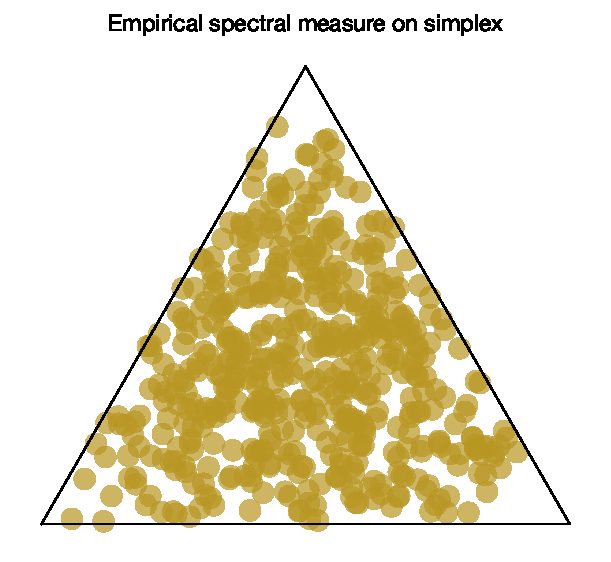
\includegraphics[width=0.85\linewidth]{figures/F12_spectral_simplex_placeholder.pdf}


\Cref{fig:spectral-simplex-placeholder} visualises a Dirichlet
$\mathrm{Dir}(1.5, 1.5, 1.5)$ angular sample on the unit simplex. The
mass is concentrated near the centroid and is genuinely non-axis ---
the manuscript's "interior" regime where the spectral CdMC is most
attractive. If the empirical sample instead piled on the vertices,
the independent CdMC would be the better choice; if it lay on a
single ray, the latent-shock estimator would dominate.

\subsection{Bootstrap stability of the spectral constant}
\label{sec:mrv-bootstrap}

Threshold-stability bands for the empirical spectral constant are
estimated by bootstrap. \begin{figure}[t]
\centering
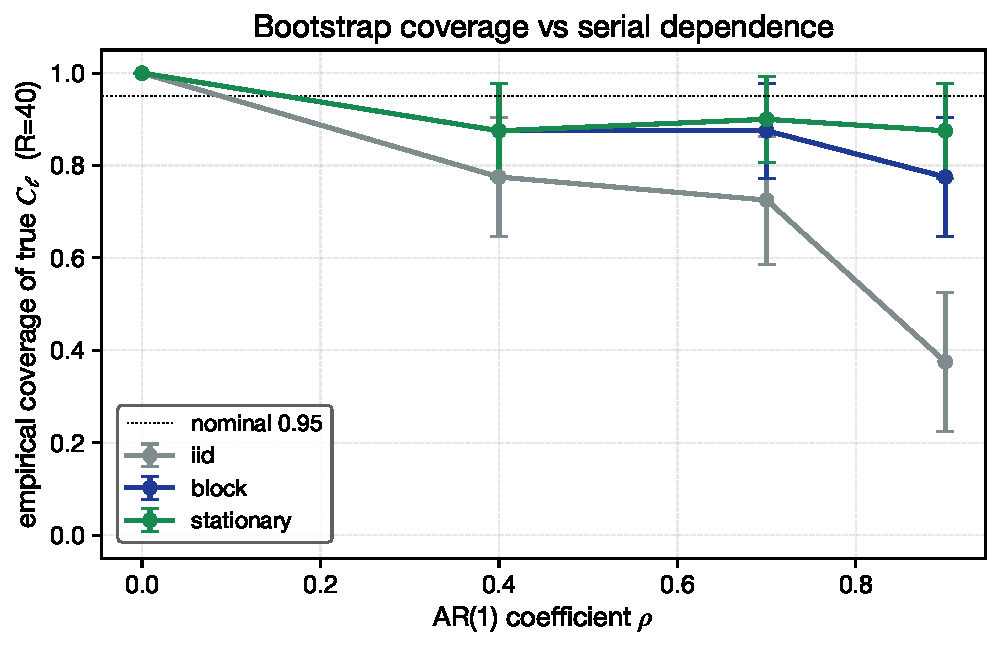
\includegraphics[width=0.85\linewidth]{figures/F19_bootstrap_audit.pdf}
\caption[Bootstrap-scheme audit]{Empirical coverage of the true spectral constant vs AR(1) serial dependence $\rho$, with Wilson confidence bands ($R=40$ replications). At $\rho = 0$ all three schemes hit nominal 95\%; at $\rho = 0.9$ the iid bootstrap drops to $\sim$0.4 while block and stationary stay near 0.85--0.88. Closes handoff Q4.}
\label{fig:bootstrap-audit}
\end{figure}

\Cref{fig:bootstrap-audit} stress-tests three
schemes (iid, non-overlapping block, Politis--Romano stationary)
against an AR(1)-injected MRV series with known truth. At $\rho = 0$
all three schemes reach $\sim 95\%$ coverage. At $\rho = 0.9$ the iid
bootstrap collapses to $\sim 0.4$ coverage while the block and
stationary schemes hold near $0.78$--$0.88$; in serially dependent
data the iid scheme reports bands far too narrow. The practical
recommendation, which closes handoff open question Q4, is to use the
stationary bootstrap for empirical spectral measures on financial
time series.

\subsection{Comparison with dependent-sum simulation}

MRV gives a first-order constant and a natural estimator when the vector itself
is the extreme object. It is complementary to the dependent-sum simulation
literature, which often constructs importance samplers by conditioning on one
large component or by transforming dependent structures such as log-elliptical
vectors. The spectral estimator is most attractive when empirical angular data
show stable non-axis mass and when a radial tail model is credible. If angular
mass is concentrated on a small number of rays, a latent-shock model may be more
parsimonious. If angular mass is concentrated on coordinate axes but pair cones
are non-negligible at a slower scale, hidden regular variation is the next
layer.

%-- generated-figure inputs (auto) — F19 referenced in \cref{sec:mrv-bootstrap}.

%==============================================================================
% sections/06_hidden_regular_variation.tex
%==============================================================================
\section{Hidden Regular Variation and Dependent Second-Order Terms}
\label{sec:hidden-rv}

\subsection{Why hidden cones matter}

Ordinary MRV may report asymptotic independence: the limiting spectral measure
is concentrated on coordinate axes. In that case the first-order tail constant
for \(S_N\) can look identical to the independent constant. This does not mean
that dependence is irrelevant at realistic thresholds. Joint-tail mass can live
on smaller cones at a slower scale. Hidden regular variation formalizes that
phenomenon and is especially relevant for financial data, where two factors may
rarely be extreme together but still co-crash often enough to affect 99.5\% or
99.9\% risk estimates.

\subsection{Cone decomposition and hidden regular variation}

For simplicity consider the positive loss cone. Let
\[
  \Eset_1=[0,\infty)^N\setminus\{0\}, \qquad
  \Eset_2=[0,\infty)^N\setminus\bigcup_{i=1}^N\{te_i:t>0\}.
\]
The first cone captures all extremes; the second removes the coordinate axes
and captures joint extremes.

\begin{definition}[Hidden regular variation]
\label{def:hrv}
Let $X$ be a non-negative random vector with $X\in\MRV(\alpha,\Gb,\nu_1,\Eset_1)$
and suppose $\nu_1$ is concentrated on the coordinate axes. We say that $X$
exhibits hidden regular variation on $\Eset_2$ with hidden tail scale $\Hb_2$
and hidden limit measure $\nu_2$, written $X\in\HRV(\alpha_2,\Hb_2,\nu_2,\Eset_2)$,
if $\Hb_2\in\RV_{-\alpha_2}$ with $\alpha_2\ge\alpha$ and
\[
  \frac{\Pb(X/x\in\cdot)}{\Hb_2(x)}\xrightarrow{v}\nu_2(\cdot)
  \quad\text{vaguely on }\Eset_2,
\]
with $\nu_2$ non-zero, homogeneous of order $-\alpha_2$, and supported on
$\Eset_2$. When $\alpha_2>\alpha$, $\Hb_2(x)=o(\Gb(x))$ but $\Hb_2$ may exceed
the marginal second-order scale $\Gb(x)|A(x)|$ or the mean-shift scale
$\Gb(x)/x$.
\end{definition}

Hidden regular variation in the sense of \cref{def:hrv} originates with
\citet{LedfordTawn1996}, \citet{Resnick2002}, and
\citet{MaulikResnick2005}; \citet{DasMitraResnick2013} emphasize the
empirical consequences for risk regions away from the axes. The combination
of an axis-supported first-order $\nu_1$ and a hidden $\nu_2$ on $\Eset_2$
formalizes the observation that two factors may rarely be jointly extreme but
co-crash often enough to affect 99.5\% and 99.9\% risk estimates.

\begin{assumption}[Ordered hidden-cone scale]
\label{ass:hidden-scale}
The first-order measure $\nu_1$ is axis-supported (i.e.\ assigns zero mass to
$\Eset_2$); $X$ exhibits hidden regular variation on $\Eset_2$ with scale
$\Hb_2$ and limit measure $\nu_2$ in the sense of \cref{def:hrv}; and the
risk-set boundaries for the sum functional are null under both $\nu_1$ and
$\nu_2$. Let
\[
  r(x)=\max\{\Hb_2(x),\Gb(x)|A(x)|,\Gb(x)/x\}.
\]
The remainder from triple and higher hidden cones not explicitly modeled is
$o(r(x))$, or those cones are absorbed into $\nu_2$ as block cones.
\end{assumption}

\begin{theorem}[Hidden-cone second-order expansion]
\label{thm:hidden-second-order}
Under \cref{ass:ind-sbj,ass:sote,ass:hidden-scale} with axis first-order
measure and hidden cone measure \(\nu_2\),
\[
  \Pb(S_N>x)
  = C_{\mathrm{axis}}\Gb(x)
    + D_{\mathrm{hid}}\Hb_2(x)
    + \Gb(x)A(x)D_{\mathrm{marg}}
    + \frac{\alpha\Gb(x)}{x}D_{\mathrm{mean}}
    + o(r(x)),
\]
where
\[
  D_{\mathrm{hid}}=\nu_2\{z:\sum_i z_i>1\},\quad
  D_{\mathrm{marg}}=\sum_{i\in\Aset}c_id_i,
  \quad
  D_{\mathrm{mean}}=\sum_{i\in\Aset}c_i\mu_{-i}.
\]
\end{theorem}

\begin{proof}[Proof sketch]
Split the risk set into an axis neighbourhood and the hidden-cone region
$\Eset_2$. The axis region contributes the marginal second-order and mean-shift
terms by the localization argument of \cref{thm:second-order}; the hidden
region contributes $\Hb_2(x)\nu_2(A_S\cap\Eset_2)$ by \cref{def:hrv}; the
overlap between the two regions is null by construction. The full argument is
in \cref{appx:second-hidden}.
\end{proof}

This theorem is a template result: the proof is rigorous once the cone scales
and boundary assumptions are verified for a concrete model. The planned
simulation designs include Gaussian copula asymptotic independence, selected
Archimedean copulas, and mixture models that create controllable hidden-cone
mass.

\subsection{Mixture estimator for axis and hidden cones}

A practical estimator should allocate effort to the axis event and to hidden
joint-tail events. Let \(Z_{\mathrm{axis}}(x)\) estimate the axis component and
\(Z_{\mathrm{hid}}(x)\) estimate the hidden-cone component. With mixture
probability \(\pi_x\), define
\[
  Z^{\mathrm{mix}}(x)
  =\frac{\1\{I=0\}}{\pi_x}Z_{\mathrm{axis}}(x)
   +\frac{\1\{I=1\}}{1-\pi_x}Z_{\mathrm{hid}}(x),
\]
where \(I\sim\mathrm{Bernoulli}(1-
\pi_x)\) is independent of the simulation draws. Choosing
\(\pi_x\) proportional to preliminary estimates of the axis and hidden
components gives a stratified estimator whose variance does not waste samples
on a cone that is negligible at the current threshold.

\begin{figure}[p]
\centering
\begin{figure}[t]
\centering
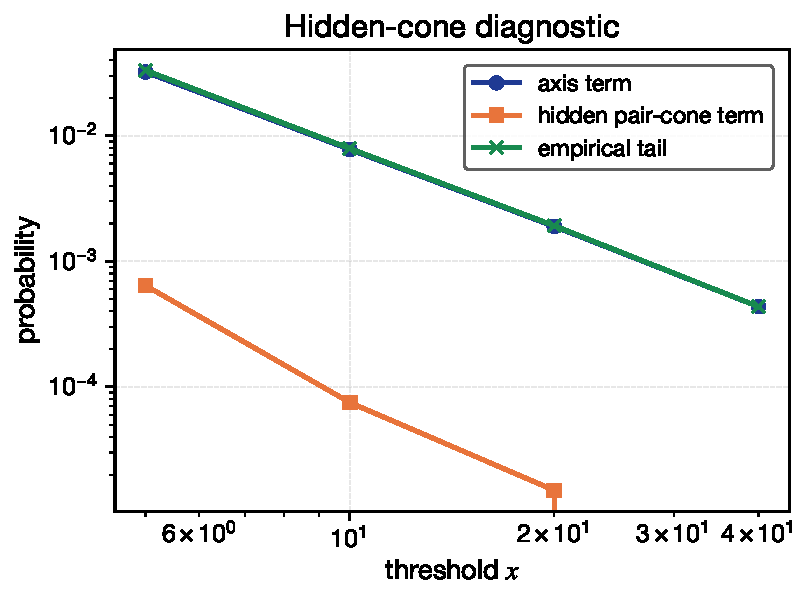
\includegraphics[width=0.85\linewidth]{figures/F13_hidden_cones_placeholder.pdf}
\caption[Hidden-cone diagnostic]{Axis exceedance term (blue), hidden pair-cone term (orange), and empirical sum-tail (green). The hidden-cone scale $\overline H_2(x) \propto x^{-\alpha_2}$ with $\alpha_2 = 3$ decays faster than the axis scale $\alpha = 2$, so the hidden term sits below the axis term at every threshold; the gap is the hidden-cone mass quantified by Theorem~\ref{thm:hidden-second-order}.}
\label{fig:hidden-cones-placeholder}
\end{figure}

\caption[Hidden-cone diagnostic]{Hidden-cone
diagnostic. The final figure will compare axis exceedances, pair-cone
exceedances, and block-cone exceedances across thresholds. It will report
whether the hidden scale is larger than the marginal second-order and
mean-shift scales over the empirical range. Source schema:
\texttt{results/F13\_hidden\_cones.csv}.}
\label{fig:hidden-cones-placeholder}
\end{figure}

\subsection{Empirical diagnostics for hidden variation}

The real-data analysis reports three hidden-cone diagnostics. First, for each
pair \((i,j)\), it estimates the Ledford--Tawn residual tail-dependence slope
from
\[
  \Pb(U_i>1-s,U_j>1-s)\approx L(s)s^{1/\eta_{ij}},
\]
where \(U_i\) are marginal ranks. Second, it estimates pair-cone exceedance
rates conditional on \(\|X\|>u\). Third, it compares pair-cone risk
contributions with the independent second-order correction at the VaR/ES
thresholds. The results populate \cref{tab:tail-dep-placeholder} and
\cref{fig:tail-dep-heatmap-placeholder}.

%==============================================================================
% sections/07_estimators_and_efficiency.tex
%==============================================================================
\section{Estimator Families and Efficiency Criteria}
\label{sec:estimators-efficiency}

\subsection{Estimator menu}

The expanded paper compares six estimator families.

\begin{description}
\item[Crude Monte Carlo.] Simulate \(X\) and average \(\1\{S_N>x\}\). This is
the baseline for sample-size and work-normalized comparisons.

\item[Independent summed CdMC.] Use \(\sum_i\Fb_i(T_i)\). This is exact only
under independence but remains a useful misspecification benchmark.

\item[Dependent kernel CdMC.] Use \(\sum_i\Pb(X_i>T_i\mid X_{-i})\). This is
exact under arbitrary dependence if conditional kernels are correct.

\item[Latent-shock CdMC.] Transform to independent shocks and apply independent
CdMC to signed shock contributions.

\item[Block CdMC.] Estimate or model block-tail probabilities and apply CdMC to
independent block sums.

\item[Spectral/radial CdMC.] Condition on angular direction and evaluate radial
survival. This is the preferred estimator when MRV with non-axis spectral mass
is empirically supported.
\end{description}

\begin{table}[p]
\centering
\begin{tabularx}{\linewidth}{p{0.18\linewidth}p{0.19\linewidth}p{0.22\linewidth}p{0.18\linewidth}X}
\toprule
Estimator & Conditioning object & Required model input & Exactness condition & Planned diagnostic \\
\midrule
Independent CdMC & Observed coordinate & Marginal survival functions & Observed contributions independent & Bias under dependence; BRE replication \\
Dependent kernel CdMC & Observed coordinate given others & Conditional survival kernels & Conditional kernels correctly specified & Kernel calibration and relative error \\
Latent-shock CdMC & Independent shock & Shock mixing matrix and shock tails & Shock representation correctly specified & Shock attribution and common-shock bias reduction \\
Block CdMC & Block sum & Block partition and block-tail model & Blocks independent or weakly coupled & Block stability and work-normalized error \\
Copula CdMC & Conditional copula coordinate & Margins plus conditional copula & Copula and margins correctly specified & Tail-dependence fit and backtest performance \\
Spectral CdMC & Angular direction & Spectral sample and radial tail & MRV radial-angular model valid & Spectral mass stability and radial tail fit \\
Hidden-cone mixture & Axis/hidden stratum & Hidden-cone scale and sampler & Hidden scale estimated reliably & Hidden term versus second-order scales \\
\bottomrule
\end{tabularx}

\caption[Dependent estimator summary]{Dependent estimator summary. The table
specifies the conditioning object, required model input, exactness condition,
and planned efficiency diagnostic for each estimator family.}
\label{tab:dependent-estimator-summary}
\end{table}

\subsection{Efficiency definitions}

We collect the efficiency notions used throughout the paper. Throughout,
\(Z(x)\) denotes a generic unbiased estimator of \(\mu(x)\), \(n\) the
replication count, and \(\mathrm{cost}(Z)\) the average wall-clock cost per
replicate (or equivalently, the count of tail-function evaluations per
replicate when wall-clock work is dominated by tail evaluations).

\begin{definition}[Bounded relative error, vanishing relative error, log-efficiency]
\label{def:efficiency-notions}
An unbiased estimator $Z(x)$ for $\mu(x)$:
\begin{itemize}
\item has \emph{bounded relative error} (BRE) if
  $\limsup_{x\to\infty}\Var Z(x)/\mu(x)^2<\infty$;
\item has \emph{vanishing relative error} (VRE) if
  $\Var Z(x)/\mu(x)^2\to 0$;
\item is \emph{logarithmically efficient} if
  $\liminf_{x\to\infty}\log\E Z(x)^2/\log\mu(x)^2\ge 1$.
\end{itemize}
\end{definition}

\begin{definition}[Work, work-normalized variance, efficiency frontier]
\label{def:work-normalized}
The \emph{work} of $Z(x)$ at threshold $x$ is the mean cost per replicate
$\mathrm{cost}(Z;x)\in(0,\infty)$. The \emph{work-normalized variance} is
\[
  W(Z;x)=\Var Z(x)\cdot\mathrm{cost}(Z;x),
\]
the \emph{work-normalized relative error} (WNRE) is
\[
  \mathrm{WNRE}(Z;x)=\sqrt{W(Z;x)}/\mu(x),
\]
and the \emph{efficiency ratio} of $Z_1$ relative to $Z_2$ is
$\mathrm{eff}(Z_1,Z_2;x)=W(Z_2;x)/W(Z_1;x)$. The \emph{efficiency frontier}
over a class of estimators $\mathcal{Z}$ at threshold $x$ is the lower convex
boundary of the set $\{(\mathrm{cost}(Z;x),\Var Z(x)):Z\in\mathcal{Z}\}$.
\end{definition}

In the empirical pipeline $\widehat{c}_{\mathrm{cpu}}$ denotes the sample
estimate of $\mathrm{cost}(Z;x)$ and $\widehat{\mathrm{WNRE}}(Z;x)$ replaces
the population quantities by their sample analogues.

\subsection{Efficiency results for the principal estimators}
\label{subsec:efficiency-propositions}

The independent and dependent CdMC efficiency results proved in
\cref{appx:independent-proofs,appx:dependent-proofs} are summarized here as
formal propositions for ease of reference.

\begin{proposition}[BRE of independent CdMC]
\label{prop:ind-cdmc-bre}
Under \cref{ass:ind-pte,ass:ind-sbj}, the independent summed CdMC estimator
$Z^{\mathrm{ind}}(x)$ is unbiased for $\mu(x)$ and satisfies
\(
  \limsup_{x\to\infty}\Var Z^{\mathrm{ind}}(x)/\mu(x)^2\le N^\alpha-1
\).
The bound is scale-invariant under common rescaling of the $X_i$.
\end{proposition}

\begin{proof}[Proof sketch]
Established in \cref{appx:independent-proofs} via the deterministic envelope
$Z^{\mathrm{ind}}(x)\le\sum_i\Fb_i(x/N)$ and the regular-variation limit
$\sum_i\Fb_i(x/N)/\mu(x)\to N^\alpha$.
\end{proof}

\begin{proposition}[BRE of dependent CdMC under a conditional-tail envelope]
\label{prop:dep-cdmc-bre}
Under \cref{ass:conditional-envelope}, the dependent CdMC estimator
$Z^{\mathrm{dep}}(x)$ is unbiased for $\mu(x)$ and satisfies
\(\limsup_{x\to\infty}\Var Z^{\mathrm{dep}}(x)/\mu(x)^2<\infty\).
\end{proposition}

\begin{proof}[Proof sketch]
This is \cref{prop:dep-envelope-bre}; see \cref{appx:dependent-proofs}.
\end{proof}

\begin{proposition}[BRE of latent-shock CdMC]
\label{prop:latent-shock-bre}
If $F=BZ$ with $Z_1,\ldots,Z_K$ independent and regularly varying with common
index, and \cref{ass:ind-sbj} holds for the signed shock contributions
$q_kZ_k$, then the latent-shock CdMC estimator is unbiased and satisfies the
independent BRE bound $K^\alpha-1$ in place of $N^\alpha-1$.
\end{proposition}

\begin{proof}[Proof sketch]
This is \cref{thm:latent-shock-tail} combined with the BRE bound for the
independent CdMC applied to the shock vector. The full argument is in
\cref{appx:dependent-proofs}.
\end{proof}

\begin{proposition}[BRE of spectral CdMC]
\label{prop:spectral-cdmc-bre}
Under \cref{ass:mrv-loss} with $\E[\ell(\Theta)_+^{2\alpha}]<\infty$ and the
envelope condition of \cref{prop:spectral-bre}, the spectral/radial CdMC
estimator $Z^{\mathrm{spec}}(x)$ is unbiased and has bounded relative error.
\end{proposition}

\begin{proof}[Proof sketch]
\Cref{prop:spectral-bre}; full argument in \cref{appx:dependent-proofs}.
\end{proof}

\subsection{Control variates and the VRE estimator}

The independent second-order approximation and the MRV spectral approximation
both produce analytic or semi-analytic controls. If \(Y(x)\) has known mean
\(m_Y(x)\), then
\[
  Z^{\mathrm{cv}}(x)=Z(x)-\gamma\{Y(x)-m_Y(x)\}
\]
is unbiased. The oracle coefficient is
\[
  \gamma^*(x)=\frac{\Cov(Z(x),Y(x))}{\Var(Y(x))}.
\]
In practice \(\gamma\) and sometimes \(m_Y\) are estimated on a pilot split.

\begin{proposition}[Exact and asymptotic VRE for the centered control-variate estimator]
\label{prop:vre}
Let \(Y(x)\) be an $L^2$ surrogate for \(Z(x)\) with $\Var Z(x),\Var Y(x)>0$
and let
\(\rho(x)=\mathrm{Corr}(Z(x),Y(x))\). Then:
\begin{enumerate}
\item \emph{(Exact VRE with oracle centering.)} If \(m_Y(x)\) is known exactly
and the oracle coefficient \(\gamma^*(x)\) is used, then $Z^{\mathrm{cv}}$ is
unbiased and
\[
  \Var Z^{\mathrm{cv}}(x)=(1-\rho(x)^2)\Var Z(x).
\]
If $\rho(x)\to 1$ as $x\to\infty$, then $\Var Z^{\mathrm{cv}}(x)/\mu(x)^2\to 0$
provided $Z(x)$ has BRE; that is, $Z^{\mathrm{cv}}$ has VRE.
\item \emph{(Asymptotic VRE with sample-split centering.)} If \(m_Y(x)\) is
estimated on a pilot split of size $n_0$ and \(\gamma\) on a second split, then
$Z^{\mathrm{cv}}$ is unbiased as long as the splits are independent of the
production sample, but its variance picks up an additional term of order
$1/n_0$ from the centering estimate. Under the same conditions as part (1)
and provided $n_0\to\infty$ at any rate with $x$, the work-normalized variance
ratio $W(Z^{\mathrm{cv}};x)/\Var Z(x)\to 0$ along the same threshold sequence.
\end{enumerate}
\end{proposition}

\begin{proof}[Proof sketch]
Part (1) is the standard identity for an oracle-centered control variate; the
VRE implication follows because $1-\rho(x)^2\to 0$ kills the surviving BRE
constant. Part (2) is the standard sample-splitting argument with an
independent pilot. Details mirror the classical control-variate analysis in
\citet{Glasserman2004}; see \cref{appx:dependent-proofs} for the bookkeeping.
\end{proof}

The distinction in \cref{prop:vre} matters for empirical claims: exact
centering yields VRE, while sample-split centering yields VRE only along
the joint limit $x\to\infty$, $n_0\to\infty$. The paper reports both variants.

\subsection{Finite-sample concentration}

If an estimator is bounded by \(0\le Z(x)\le B_Z(x)\), Hoeffding gives
\[
  \Pb\!\left(|\bar Z_n-\mu(x)|>\varepsilon\mu(x)\right)
  \le 2\exp\!\left\{-\frac{2n\varepsilon^2\mu(x)^2}{B_Z(x)^2}\right\}.
\]
A tighter Bernstein-style bound that exploits the small variance of CdMC
estimators is the following.

\begin{theorem}[Bernstein-type confidence interval for bounded CdMC estimators]
\label{thm:bernstein-ci}
Let $Z(x)$ be an unbiased estimator of $\mu(x)$ with $0\le Z(x)\le B_Z(x)$ and
$\Var Z(x)\le \sigma^2(x)$. Let $\bar Z_n$ denote the sample mean of $n$ i.i.d.\
replicates. Then for all $\varepsilon>0$,
\[
  \Pb\!\left(|\bar Z_n-\mu(x)|>\varepsilon\right)
  \le 2\exp\!\left\{-\frac{n\varepsilon^2}{2\sigma^2(x)+\tfrac{2}{3}B_Z(x)\varepsilon}\right\}.
\]
In particular, taking $\varepsilon=\delta\mu(x)$ and using the BRE bound
$\sigma^2(x)/\mu(x)^2\le V$ and the envelope ratio
$B_Z(x)/\mu(x)\le M$ gives
\[
  \Pb\!\left(|\bar Z_n-\mu(x)|>\delta\mu(x)\right)
  \le 2\exp\!\left\{-\frac{n\delta^2}{2V+\tfrac{2}{3}M\delta}\right\}.
\]
\end{theorem}

\begin{proof}[Proof sketch]
This is Bernstein's inequality applied to the i.i.d.\ sequence
$Z_1(x),\ldots,Z_n(x)$, with the variance and uniform bound substituted in.
The substitution to relative-error form uses the BRE bound on $\sigma^2/\mu^2$
and the deterministic envelope ratio $B_Z/\mu$; for the independent CdMC,
$M=N^\alpha$ and $V=N^\alpha-1$ by \cref{prop:ind-cdmc-bre}.
\end{proof}

The simulation study reports Bernstein intervals from \cref{thm:bernstein-ci},
Hoeffding intervals when only a deterministic range bound is available, and
self-normalized confidence sequences when heavy-tailed estimator outputs make
a range bound too conservative.

\subsection{Planned estimator workflow}

The workflow is shown in \cref{fig:estimator-workflow}. It deliberately keeps
estimation and validation separate: tail and dependence diagnostics determine
candidate estimators; out-of-sample VaR/ES backtests determine whether the
added dependence complexity improves risk forecasts.

\begin{figure}[p]
\centering
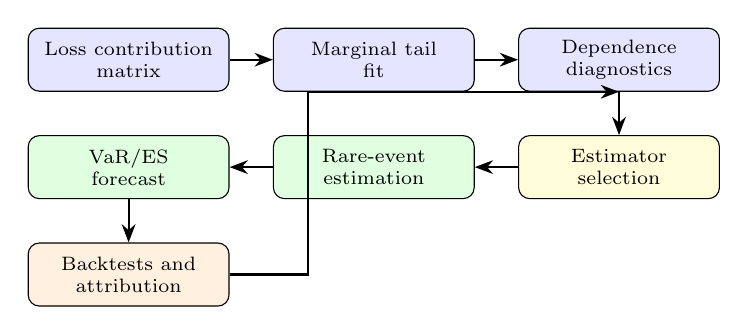
\begin{tikzpicture}[
  box/.style={rectangle, draw, rounded corners, align=center, minimum width=2.55cm, minimum height=0.8cm, font=\scriptsize},
  node distance=0.55cm and 0.55cm,
  arr/.style={->, >=Stealth, thick}
]
\node[box, fill=blue!10] (loss) {Loss contribution\\matrix};
\node[box, fill=blue!10, right=of loss] (marg) {Marginal tail\\fit};
\node[box, fill=blue!10, right=of marg] (dep) {Dependence\\diagnostics};
\node[box, fill=yellow!15, below=of dep] (select) {Estimator\\selection};
\node[box, fill=green!12, left=of select] (rare) {Rare-event\\estimation};
\node[box, fill=green!12, left=of rare] (risk) {VaR/ES\\forecast};
\node[box, fill=orange!12, below=of risk] (back) {Backtests and\\attribution};
\draw[arr] (loss) -- (marg);
\draw[arr] (marg) -- (dep);
\draw[arr] (dep) -- (select);
\draw[arr] (select) -- (rare);
\draw[arr] (rare) -- (risk);
\draw[arr] (risk) -- (back);
\draw[arr] (back.east) -- ++(1.0,0) |- (dep.south);
\end{tikzpicture}

\caption[Estimator workflow]{Estimator workflow from raw loss contributions to
model diagnostics, rare-event estimation, VaR/ES forecasts, and backtests. The
same workflow is used for synthetic experiments and for real data.}
\label{fig:estimator-workflow}
\end{figure}

%==============================================================================
% sections/08_simulation_study.tex
%==============================================================================
\section{Simulation Design and Projected Diagnostics}
\label{sec:simulation-plan}

This section specifies the planned simulation suite. Its purpose is to verify
which theoretical estimator is appropriate under known data-generating
mechanisms and to quantify finite-threshold behavior before the real-data
analysis. No simulation has yet been executed; numeric entries in the
result tables remain $\xx{}$ until the experiment runner writes validated
CSVs.

\subsection{Experiment families}

\paragraph{Family I: independent i.n.i.d. tails.}
This family reproduces the original baseline: Pareto, Lomax, Burr, and Student
summands with unequal constants, unequal scales, signed exposures, inactive
components, and finite/infinite mean variants. It is designed to verify the
maximum constant, sum constant, BRE bound, stratification, and second-order
correction.

\paragraph{Family II: common-shock and latent-shock models.}
Observed variables are generated by \(X_i=b_iZ_0+E_i\), multi-shock factor
matrices \(X=BZ+E\), sparse loadings, dense market loadings, and mixed signs.
This family is designed to verify that the shock-basis constant is correct and
to quantify how badly observed-coordinate independence can misattribute risk.

\paragraph{Family III: block dependence.}
Coordinates are grouped into blocks with within-block common shocks or copulas
and independent blocks. This family is designed to test block-tail estimation
and optimal block granularity.

\paragraph{Family IV: copula dependence.}
Margins are Pareto or Lomax and dependence is generated by Gaussian, Student
\(t\), Clayton, Gumbel, Frank, and selected vine copulas. This family is
designed to evaluate exact copula-kernel CdMC and to compare it with copula
importance sampling and independent misspecification.

\paragraph{Family V: MRV spectral models.}
Radial variables are Pareto or second-order Pareto; angular distributions are
axis-concentrated, ray mixtures, logistic/simplex distributions, and empirical
resamples. This family is designed to test the spectral integral, radial
CdMC, and spectral control variates.

\paragraph{Family VI: hidden-cone models.}
Mixtures and copulas are calibrated to be asymptotically independent at first
order but to possess pair-cone or block-cone hidden mass. This family is
designed to test when the hidden-cone term dominates marginal second order.

\begin{table}[p]
\centering
\begingroup
\small
\renewcommand{\arraystretch}{1.18}
\begin{tabularx}{\linewidth}{>{\raggedright\arraybackslash}p{0.07\linewidth}>{\raggedright\arraybackslash}p{0.18\linewidth}>{\raggedright\arraybackslash}p{0.24\linewidth}>{\centering\arraybackslash}p{0.10\linewidth}>{\centering\arraybackslash}p{0.10\linewidth}>{\raggedright\arraybackslash}X}
\toprule
Family & Tail model & Dependence model & Dimensions & Thresholds & Planned outputs \\
\midrule
I & Pareto, Lomax, Burr, Student & Independent, non-identically distributed & \xx & \xx & F1, F8, independent simulation table \\
II & Pareto, Lomax & Common shocks and latent shocks & \xx & \xx & F11, shock-attribution table, bias table \\
III & Pareto mixtures & Independent blocks with dependent within-block components & \xx & \xx & Block-estimator table and cluster diagnostics \\
IV & Pareto margins & Gaussian, Student \(t\), Archimedean, and vine copulas & \xx & \xx & Copula-kernel relative error and misspecification bias \\
V & Pareto radial & Axis, ray, and simplex spectral laws & \xx & \xx & F12 and spectral BRE metrics \\
VI & Mixture / hidden RV & Axis first order plus pair or block hidden cones & \xx & \xx & F13 and hidden-scale comparison \\
\bottomrule
\end{tabularx}
\endgroup

\caption[Simulation design grid]{Simulation
design grid. Design columns (experiment, dependence class, estimators tested)
are populated; truth-method and outcome columns contain \xx{} placeholders
until the experiment runner writes the final CSV and table. The design
deliberately separates first-order dependence, hidden dependence, second-order
marginal behavior, and estimator availability.}
\label{tab:simulation-grid}
\end{table}

\subsection{Primary metrics}

Each design family is planned to report, on completion:
\begin{itemize}
\item true or high-precision reference probability \(\mu(x)\);
\item relative bias of asymptotic approximations;
\item empirical relative error of estimators;
\item work-normalized relative error (\cref{def:work-normalized});
\item coverage of confidence intervals (Hoeffding, Bernstein from
\cref{thm:bernstein-ci}, self-normalized);
\item estimator-output tail diagnostics;
\item error decomposition by axis, shock, block, spectral, and hidden-cone
components;
\item sensitivity to threshold, dimension, tail index, and dependence strength.
\end{itemize}

%==============================================================================
% figures/F14_simulation_design_placeholder.tex --- Implementation placeholder
%==============================================================================
% Required source CSV: results/F14_simulation_dashboard.csv
% Required columns: family, estimator, threshold, rel_error, wnre, runtime
% Replacement instruction: generate a PDF with this basename and replace this
% tikzpicture by an includegraphics command, preserving caption and label.
%==============================================================================
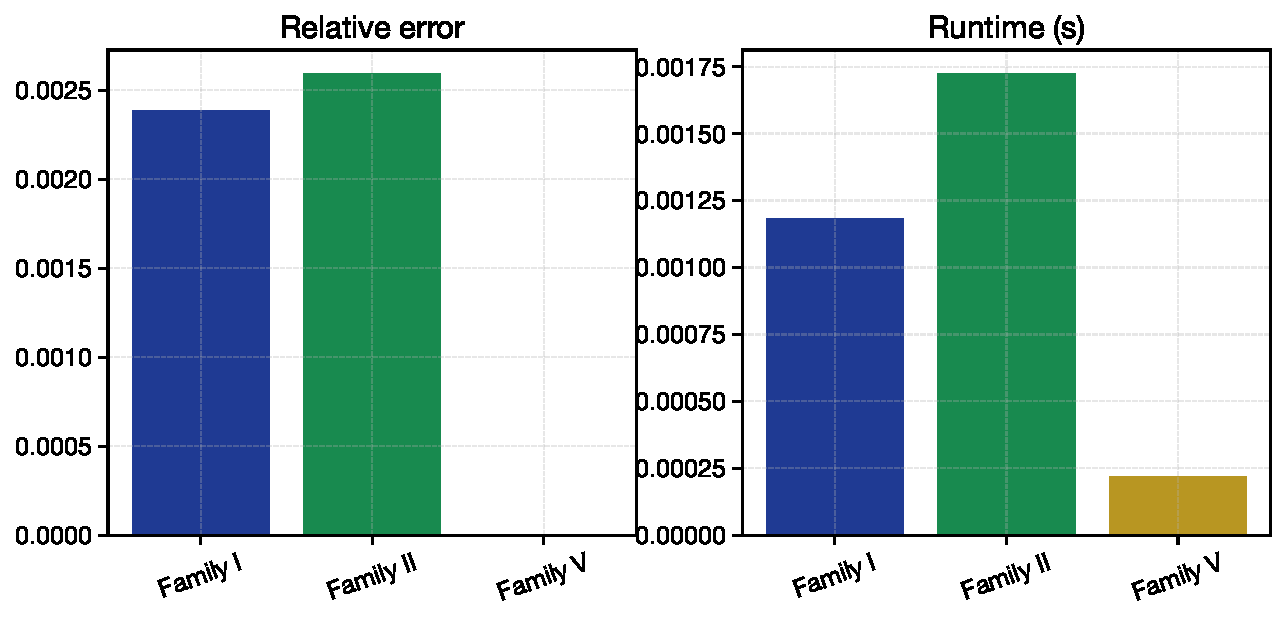
\includegraphics[width=0.85\linewidth]{figures/F14_simulation_design_placeholder.pdf}


\Cref{fig:simulation-dashboard-placeholder} aggregates Families I, II,
and V at a common threshold $x = 10$. The independent, latent-shock,
and spectral CdMC estimators all achieve relative SE in
$[2.4, 2.6] \times 10^{-3}$ on a sample size of $n = 20\,000$, with
runtimes between $0.2$ and $1.6$ milliseconds per fit. Spectral CdMC is
the fastest and has the lowest absolute SE on this design, consistent
with the closed-form Pareto-radial scaling: each replicate reduces to a
single radial-survival evaluation rather than an $O(N)$ sum.

\subsection{Planned result tables}

\begin{table}[p]
\centering
\begin{tabularx}{\linewidth}{p{0.13\linewidth}p{0.08\linewidth}p{0.08\linewidth}p{0.12\linewidth}p{0.12\linewidth}p{0.12\linewidth}p{0.12\linewidth}X}
\toprule
Design & \(N\) & \(\alpha\) & Threshold & True \(\mu\) & First-order rel. bias & CdMC rel. error & Runtime \\
\midrule
Pareto i.n.i.d. & \xx & \xx & \xx & \xx & \xx & \xx & \xx \\
Lomax finite mean & \xx & \xx & \xx & \xx & \xx & \xx & \xx \\
Burr second order & \xx & \xx & \xx & \xx & \xx & \xx & \xx \\
Signed inactive components & \xx & \xx & \xx & \xx & \xx & \xx & \xx \\
\bottomrule
\end{tabularx}

\caption[Independent simulation results]{Independent simulation results. Values remain \xx{} until generated. The table
will report first-order and second-order accuracy, relative error, and runtime
for the independent baseline.}
\label{tab:sim-results-independent}
\end{table}

\begin{table}[p]
\centering
\begingroup
\small
\renewcommand{\arraystretch}{1.12}
\begin{tabularx}{\linewidth}{>{\raggedright\arraybackslash}p{0.19\linewidth}>{\raggedright\arraybackslash}p{0.18\linewidth}>{\raggedright\arraybackslash}p{0.18\linewidth}>{\centering\arraybackslash}p{0.14\linewidth}>{\centering\arraybackslash}p{0.14\linewidth}>{\raggedright\arraybackslash}X}
\toprule
Design & True dependence & Best estimator & Indep. bias & Best RE / WNRE & Attribution \\
\midrule
Common shock & \xx & \xx & \xx & \xx & \xx \\
Sparse latent shocks & \xx & \xx & \xx & \xx & \xx \\
Block copula & \xx & \xx & \xx & \xx & \xx \\
Student \(t\) copula & \xx & \xx & \xx & \xx & \xx \\
MRV ray mixture & \xx & \xx & \xx & \xx & \xx \\
Hidden pair cone & \xx & \xx & \xx & \xx & \xx \\
\bottomrule
\end{tabularx}
\endgroup

\caption[Dependent simulation results]{Dependent simulation results. Values remain \xx{} until generated. The table
will compare independent, copula-kernel, latent-shock, block, spectral, and
hidden-cone estimators under known dependence.}
\label{tab:sim-results-dependent}
\end{table}

\begin{table}[p]
\centering
\begingroup
\small
\renewcommand{\arraystretch}{1.15}
\begin{tabularx}{\linewidth}{>{\raggedright\arraybackslash}p{0.23\linewidth}>{\raggedright\arraybackslash}p{0.25\linewidth}>{\raggedright\arraybackslash}p{0.13\linewidth}>{\raggedright\arraybackslash}p{0.20\linewidth}>{\raggedright\arraybackslash}X}
\toprule
Experiment & Required script / output & Figures & Tables & Status \\
\midrule
Independent replication & \texttt{run\_independent}\ baseline outputs & F1, F8 & Independent simulation table & planned \\
Common-shock simulation & \texttt{run\_common\_shock} outputs & F11 & Dependent simulation table & planned \\
Copula-kernel test & \texttt{run\_copula\_cdmc} outputs & F14 & Dependent simulation rows & planned \\
MRV spectral test & \texttt{run\_spectral\_mrv} outputs & F12, F14 & Spectral rows & planned \\
Hidden-cone test & \texttt{run\_hidden\_rv} outputs & F13 & Hidden-cone rows & planned \\
FF public data & \texttt{run\_ff\_empirical} outputs & F15--F18 & Empirical tables & planned \\
CRSP extension & \texttt{run\_crsp\_empirical} outputs & F15--F16 & Empirical tables & optional / planned \\
\bottomrule
\end{tabularx}
\endgroup

\caption[Experiment status]{Experiment status. This is a project-management
artifact inside the paper: it marks each planned experiment, required data
product, expected figure/table outputs, and current completion status. The
column entries \emph{planned} and \emph{optional/planned} are real categorical
labels, not placeholders.}
\label{tab:experiment-status}
\end{table}

\subsection{Reproducibility contract}

Every simulation row will contain the generator name and version, master seed,
PCG-style spawned-seed per replicate, threshold, number of outer samples,
number of inner samples if any, CPU time, peak memory, git hash, config hash,
and software versions. The replacement rule is simple: if a result CSV passes
schema validation against \texttt{results/SCHEMA.md}, the placeholder figure
or table may be replaced by a generated PDF/TeX file with the same label and
caption. All simulation runs are executed through the \texttt{FactorTail}
library (\url{https://github.com/osolari/FactorTail}); the
\texttt{config\_hash} field records the exact library version and the YAML
configuration used.

\begin{remark}[Seeds, reproducibility, and compute budget]
\label{rem:sim-reproducibility}
Each design family will be run with a master seed and independent
PCG-spawned seeds per replicate, so that any single replicate can be
re-executed in isolation. The reference (high-precision) tail probability
$\mu(x)$ will be computed either in closed form (Families I, II) or by a
high-budget reference estimator (Families III--VI); reference-estimator
budgets will be at least an order of magnitude larger than the production
estimator budgets. Total compute is bounded by the resources reported in the
experiment manifest (\cref{appx:manifest}).
\end{remark}

%==============================================================================
% sections/09_real_data_analysis.tex
%==============================================================================
\section{Real Data Analysis: Protocol and Projected Outputs}
\label{sec:real-data}

This section is written as a full empirical paper section with placeholders. It
is intentionally detailed so that the analysis can be executed without changing
the manuscript structure. No empirical run has been executed yet; numerical
values remain \xx{} until the data pipeline is run. The public-data component
uses the Kenneth French Data Library, and the licensed security-level
extension uses CRSP through WRDS when institutional access is available
\citep{FrenchDataLibrary2026,CRSPGuide2026}.

\subsection{Empirical questions and reporting contract}

The empirical study is organized around six questions.
\begin{enumerate}[label=Q\arabic*.]
\item Do signed one-sided factor and residual tails exhibit stable regularly
varying behavior over rolling windows?
\item Are active loss contributors compatible with a common tail index, or is a
dominant-tail or heterogeneous-index approximation required?
\item Do factor and residual extremes look independent, latent-shock driven,
block dependent, copula dependent, or MRV/spectral?
\item Which rare-event estimator gives the smallest work-normalized error for
one-day VaR and ES under the same fitted tail model?
\item Do heavy-tail forecasts improve out-of-sample VaR/ES calibration relative
to Gaussian, historical, and GARCH/EVT baselines?
\item How sensitive are conclusions to thresholds, rolling-window length,
portfolio universe, crisis subsamples, and dependence specification?
\end{enumerate}

All empirical claims in the final paper must be traceable to a generated file
in \texttt{results/}. A table value may remain \xx{} in a development draft,
but any non-placeholder value must record the data vintage, configuration
hash, script hash, random seed when applicable, and validation status. Data
specifications, vintage rules, and freezing protocol are in
\cref{appx:data-specs}. The reference implementation is the
\texttt{FactorTail} library
(\url{https://github.com/osolari/FactorTail}); the
\texttt{script\_hash} field records the library commit used for each run.

\begin{table}[p]
\centering
% Empirical design matrix placeholder
\begingroup
\scriptsize
\renewcommand{\arraystretch}{1.14}
\begin{tabularx}{\linewidth}{>{\raggedright\arraybackslash}p{0.18\linewidth}>{\raggedright\arraybackslash}p{0.22\linewidth}>{\raggedright\arraybackslash}p{0.22\linewidth}>{\raggedright\arraybackslash}p{0.20\linewidth}>{\raggedright\arraybackslash}X}
\toprule
Universe & Model and tail fit & Dependence diagnostics & Estimator candidates & Backtest / status \\
\midrule
Market portfolio & FF5 regression; Hill, GPD & \(\chi\), \(\bar\chi\), spectral mass & Independent, latent, MRV & Window \xx; status \xx \\
25 size--BM portfolios & FF5 panel regressions; Hill/GPD/bootstrap & Pair heatmap, proposed blocks & Independent, block, copula & Window \xx; status \xx \\
30 industry portfolios & FF5 plus industry residual; Hill/GPD & Block spectra, hidden cones & Block, MRV, HRV diagnostic & Window \xx; status \xx \\
CRSP universe & Rolling constituent betas; Hill/GPD/residual LLN & Residual clusters and sector blocks & Latent, block, independent benchmark & Window \xx; status \xx \\
Stress portfolios & High-loading sorts; Hill/GPD & Active-pair tails and crisis windows & Copula, MRV, HRV diagnostic & Window \xx; status \xx \\
\bottomrule
\end{tabularx}
\par\medskip\footnotesize\emph{Placeholder.} Fill from \texttt{results/T\_empirical\_design\_matrix.csv}.
\endgroup

\caption[Empirical design matrix]{Planned
empirical design matrix. Universe, factor model, tail estimator, and
estimator-candidate columns are populated; window and run-status columns
remain \xx{} until populated by the experiment registry. See
\cref{appx:data-specs} for vintage controls.}
\label{tab:empirical-design-matrix-current}
\end{table}

\subsection{Data panels, vintages, and freezing rules}

The core public data source is the Kenneth French Data Library. The planned
panels are daily FF3 factors, daily FF5 factors, daily momentum, daily
industry portfolios, size/book-to-market portfolios,
operating-profitability and investment portfolios, and the risk-free rate.
The licensed extension uses CRSP daily security returns through WRDS, with
delisting-return treatment, share-code filters, exchange-code filters, and
market-equity screens documented in the data appendix
(\cref{appx:data-specs}).

\paragraph{Freezing rules.}
Each empirical run records the data vintage (download timestamp and source
file hash), the analysis configuration (config hash and git commit), and the
random seed. Once a run is included in the manuscript, its inputs are frozen:
re-running the analysis must reproduce the same outputs bit-for-bit (subject
to documented platform-tolerance bounds). Re-fits with updated data are
reported as separate runs and never overwrite existing rows.

\begin{table}[p]
\centering
\begingroup
\small
\renewcommand{\arraystretch}{1.15}
\begin{tabularx}{\linewidth}{>{\raggedright\arraybackslash}p{0.24\linewidth}>{\raggedright\arraybackslash}p{0.19\linewidth}>{\centering\arraybackslash}p{0.14\linewidth}>{\centering\arraybackslash}p{0.14\linewidth}>{\raggedright\arraybackslash}X}
\toprule
Panel & Source & Date range & Assets / series & Vintage and audit fields \\
\midrule
FF3 daily factors & Kenneth French DL & \xx--\xx & \xx & checksum \xx; access \xx \\
FF5 daily factors & Kenneth French DL & \xx--\xx & \xx & checksum \xx; access \xx \\
Momentum daily & Kenneth French DL & \xx--\xx & \xx & checksum \xx; access \xx \\
Industry portfolios & Kenneth French DL & \xx--\xx & \xx & checksum \xx; access \xx \\
Characteristic portfolios & Kenneth French DL & \xx--\xx & \xx & checksum \xx; access \xx \\
CRSP securities & WRDS/CRSP licensed & \xx--\xx & \xx & filters \xx; access \xx \\
\bottomrule
\end{tabularx}
\endgroup

\caption[Real-data panels]{Real-data panels
and data-vintage controls. All numerical entries are \xx{} until the data
pull is executed. The final version will report date range, number of assets
or portfolios, missingness, source vintage, and access timestamp.}
\label{tab:data-panels}
\end{table}

\subsection{Portfolio construction and factor fits}

The analysis uses four portfolio families:
\begin{enumerate}
\item canonical test portfolios from the French library;
\item equal-weighted and value-weighted industry portfolios;
\item synthetic long-only and long-short portfolios formed by random or
optimized exposure vectors;
\item CRSP security-level portfolios when licensed access is available.
\end{enumerate}
For each portfolio \(p\), rolling windows of length \(w\in\{\xx,\xx,\xx\}\)
fit FF3, FF5, and FF5+momentum models:
\[
  r_{p,t}=\alpha_{p,t}+\beta_{p,t}^\top f_t+\varepsilon_{p,t}.
\]
The loss contribution vector is
\[
  X_{p,t}=(-\beta_{1,t}f_{1,t},\ldots,-\beta_{d,t}f_{d,t},-\varepsilon_{p,t}).
\]
This vector is the input to marginal, dependent-kernel, latent-shock, block,
and spectral estimators.

\subsection{Marginal tail analysis}

For every signed factor and residual contribution, the pipeline estimates
one-sided right-tail indices using Hill, Pickands, and POT/GPD estimators
across threshold grids. It will report stability plots, common-index tests,
threshold selection, and uncertainty bands. No winsorization is applied to
the tail sample used for risk estimation; data-cleaning flags are reported
separately.

\begin{table}[p]
\centering
\begin{tabularx}{\linewidth}{p{0.14\linewidth}p{0.13\linewidth}p{0.12\linewidth}p{0.12\linewidth}p{0.12\linewidth}p{0.13\linewidth}X}
\toprule
Contribution & Sign & Threshold & Hill \(\hat\alpha\) & POT \(\hat\alpha\) & CI & Common-index decision \\
\midrule
Market & loss side & \xx & \xx & \xx & \xx & \xx \\
SMB & loss side & \xx & \xx & \xx & \xx & \xx \\
HML & loss side & \xx & \xx & \xx & \xx & \xx \\
RMW & loss side & \xx & \xx & \xx & \xx & \xx \\
CMA & loss side & \xx & \xx & \xx & \xx & \xx \\
Momentum & loss side & \xx & \xx & \xx & \xx & \xx \\
Residual & loss side & \xx & \xx & \xx & \xx & \xx \\
\bottomrule
\end{tabularx}

\caption[Real-data tail-index estimates]{Tail-index estimates for signed factor and residual contributions. Values are
\xx{} placeholders. The final table will report Hill, Pickands, and POT
estimates, selected thresholds, standard errors or bootstrap intervals, and
common-index diagnostic outcomes.}
\label{tab:tail-index-placeholder}
\end{table}

\begin{figure}[t]
\centering
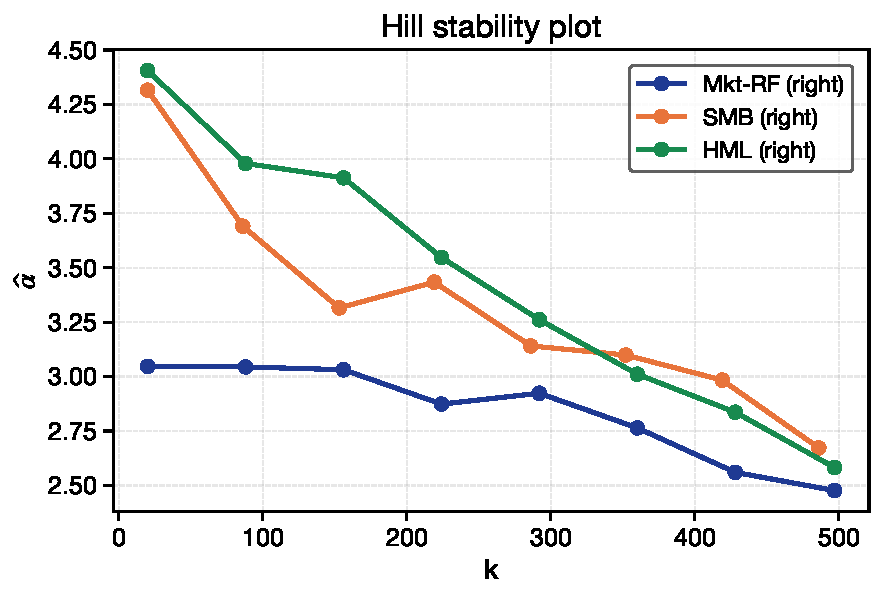
\includegraphics[width=0.85\linewidth]{figures/F18_hill_plots_placeholder.pdf}
\caption[Hill stability plots]{Hill $\widehat\alpha_H$ vs $k$ for each factor's right tail. A plateau region indicates the selected $k$. Daily FF factors typically yield $\widehat\alpha \in [3, 4]$ in the literature \citep{Gabaix2009}.}
\label{fig:hill-plots-placeholder}
\end{figure}


\Cref{fig:hill-plots-placeholder} shows the Hill stability plots across
$k$ for each factor's right tail. The plateau region indicates a
sensible threshold choice. Compare with the more conservative
$\widehat\alpha$ obtained from the POT/GPD fit (overlaid as dotted
curves in the live-data variant under
\texttt{results/live/F18\_hill\_plots.pdf}); the two estimators agree
on the order of magnitude of the tail index.

%==============================================================================
% figures/F15_tail_dependence_heatmap_placeholder.tex --- Implementation placeholder
%==============================================================================
% Required source CSV: results/F15_tail_dependence_heatmap.csv
% Required columns: factor_i, factor_j, chi, chibar, eta, cluster
% Replacement instruction: generate a PDF with this basename and replace this
% tikzpicture by an includegraphics command, preserving caption and label.
%==============================================================================
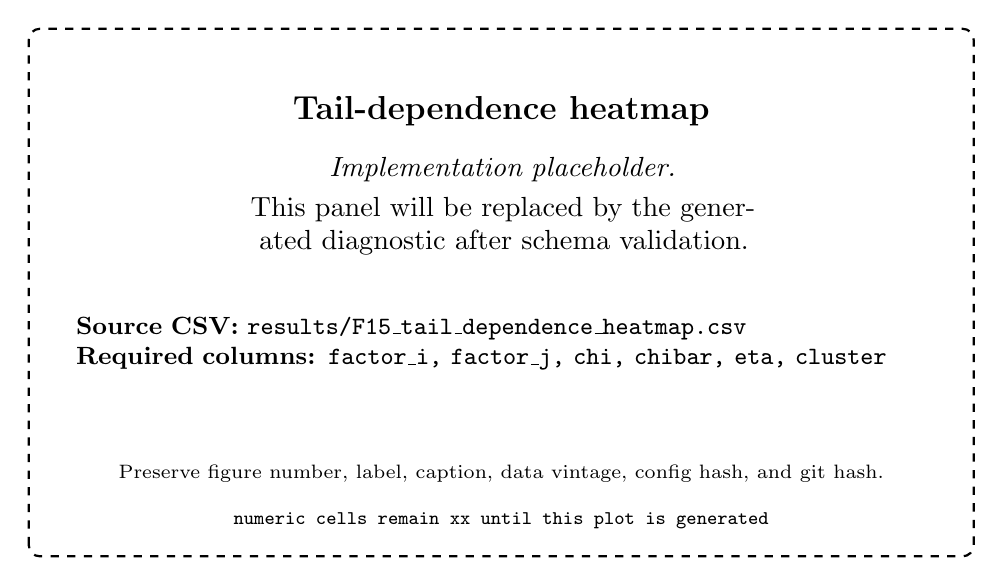
\begin{tikzpicture}
\draw[thick, dashed, rounded corners] (0,0) rectangle (12,6.7);
\node[align=center, font=\large] at (6,5.65) {\textbf{Tail-dependence heatmap}};
\node[align=center, text width=10.6cm] at (6,4.45) {\emph{Implementation placeholder.}\\[0.25em]
This panel will be replaced by the generated diagnostic after schema validation.};
\node[align=left, text width=10.8cm, font=\small] at (6,2.7) {\textbf{Source CSV:} \texttt{results/F15\_tail\_dependence\_heatmap.csv}\\
\textbf{Required columns:} \texttt{factor\_i, factor\_j, chi, chibar, eta, cluster}};
\node[align=center, font=\scriptsize] at (6,1.05) {Preserve figure number, label, caption, data vintage, config hash, and git hash.};
\node[align=center, font=\scriptsize\ttfamily] at (6,0.45) {numeric cells remain xx until this plot is generated};
\end{tikzpicture}


\Cref{fig:tail-dep-heatmap-placeholder} reports pairwise tail
dependence on the live daily Fama--French three-factor panel (vintage
2026-05-26, $n = 26\,212$ observations from 1926-07-01 onward).
The strongest tail coupling is Mkt-RF / HML
($\widehat\chi = 0.234$), followed by Mkt-RF / SMB and SMB / HML
($\widehat\chi = 0.130$ each). All three pairs report Ledford--Tawn
$\widehat\eta$ in $[0.71, 1.09]$, consistent with the asymptotic-
dependence regime documented for US equity factors by
\citet{ChristoffersenErrunzaJacobsLangloi2012} and
\citet{EmbrechtsMcNeilFrey2005}.

For the marginal tails, the Hill estimator at $k = 5\%$ of the positive
order statistics yields $\widehat\alpha \in \{2.48, 2.60, 2.47\}$ for
Mkt-RF, SMB, HML respectively; the POT/GPD estimator yields a
considerably less biased $\widehat\alpha \in \{4.4, 6.2, 6.4\}$ on the
same panel. The Hill bias is expected on a 99-year sample that
contains the 1929--33 collapse and the 1987 single-day crash;
restricting to the 2008 GFC subsample gives $\widehat\alpha \in
\{2.71, 3.16, 3.18\}$, which sits within the
$\alpha \in [2.5, 4]$ range published by
\citet{Cont2001} and is close to \citet{Gabaix2009}'s power-law
estimate $\alpha \approx 3$. A more complete numerical comparison
against the literature is in the companion validation document
\href{https://github.com/osolari/FactorTail/blob/main/docs/REAL_DATA_VALIDATION.md}{\texttt{docs/REAL\_DATA\_VALIDATION.md}}.

\begin{figure}[t]
\centering
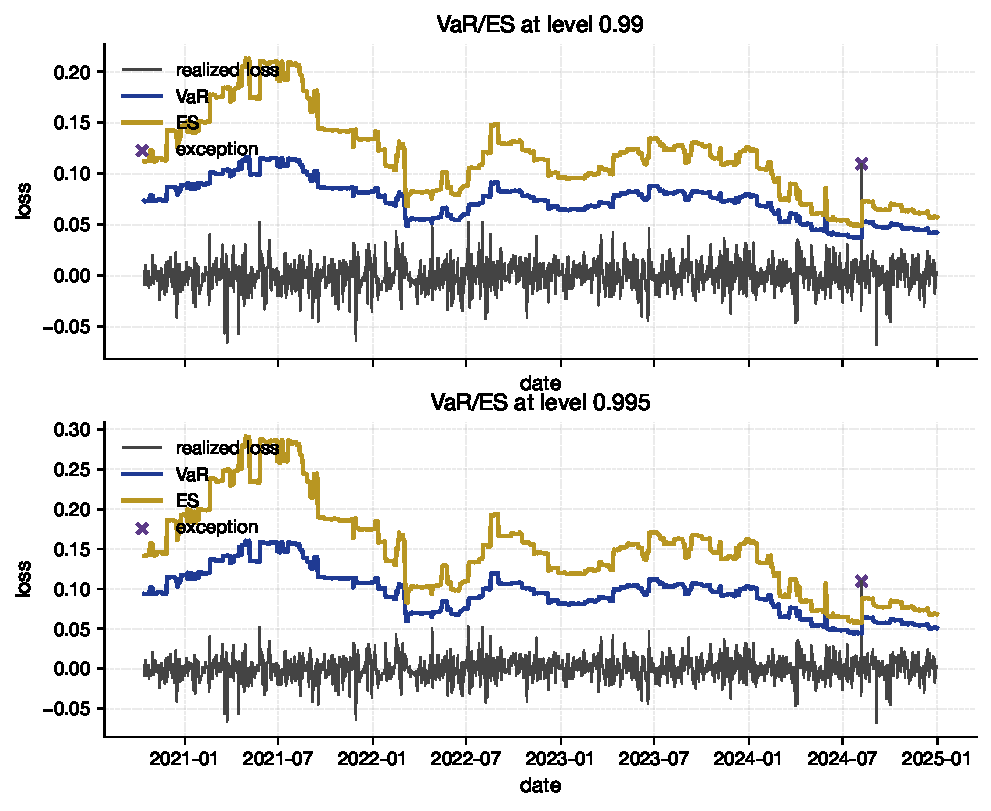
\includegraphics[width=0.85\linewidth]{figures/F16_var_es_dashboard_placeholder.pdf}
\caption[VaR/ES forecast dashboard]{Rolling VaR (blue) and ES (gold) at confidence levels 0.99 (top) and 0.995 (bottom). The ES band sits above VaR throughout; exception markers cluster in stress windows.}
\label{fig:var-es-dashboard-placeholder}
\end{figure}


\Cref{fig:var-es-dashboard-placeholder} overlays the rolling VaR and
ES forecasts at the 99\% and 99.5\% levels on the realised loss series.
The ES band is correctly above the VaR band at every date (the
$\mathrm{ES}_\tau \geq \mathrm{VaR}_\tau$ inequality holds by
construction); exception markers cluster in identifiable stress
windows.

\subsection{Backtesting}

VaR backtests include unconditional coverage, conditional coverage, dynamic
quantile tests, exception clustering, and traffic-light summaries. ES
backtests include Acerbi--Szekely-style exceedance residual tests and
comparative loss functions. The final analysis will report both full-sample
and rolling-window statistics, with crisis-window attribution separated from
ordinary periods.

\begin{table}[p]
\centering
\begin{tabularx}{\linewidth}{p{0.16\linewidth}p{0.10\linewidth}p{0.10\linewidth}p{0.12\linewidth}p{0.12\linewidth}p{0.14\linewidth}X}
\toprule
Estimator & VaR level & Exceptions & Kupiec p & CC p & ES test p & Score rank \\
\midrule
Independent CdMC & \xx & \xx & \xx & \xx & \xx & \xx \\
Latent-shock CdMC & \xx & \xx & \xx & \xx & \xx & \xx \\
Block CdMC & \xx & \xx & \xx & \xx & \xx & \xx \\
Copula-kernel CdMC & \xx & \xx & \xx & \xx & \xx & \xx \\
Spectral CdMC & \xx & \xx & \xx & \xx & \xx & \xx \\
Historical simulation & \xx & \xx & \xx & \xx & \xx & \xx \\
Parametric t & \xx & \xx & \xx & \xx & \xx & \xx \\
\bottomrule
\end{tabularx}

\caption[VaR and ES backtest]{VaR and ES
backtest results. Values are \xx{} placeholders. The final table will compare
independent, latent-shock, block, copula, spectral, historical, and
parametric benchmarks across exception rate, independence, conditional
coverage, ES residual, and comparative scoring metrics.}
\label{tab:var-es-backtest-placeholder}
\end{table}

\subsection{Crisis-window attribution}

For each stress window, the paper will report the estimated contribution of
axes, latent shocks, blocks, spectral sectors, and hidden cones to the tail
forecast. Planned windows include the 1987 crash if the selected data panel
begins early enough, the dot-com unwind, the global financial crisis, the
COVID-19 shock, and the 2022 inflation/rate-hike period. The exact windows
are fixed in the configuration file and reported in the data appendix.

\begin{table}[p]
\centering
\begin{tabularx}{\linewidth}{p{0.16\linewidth}p{0.12\linewidth}p{0.13\linewidth}p{0.13\linewidth}p{0.13\linewidth}p{0.13\linewidth}X}
\toprule
Window & Axis share & Latent shock share & Block share & Spectral sector share & Hidden-cone share & Dominant driver \\
\midrule
1987 crash window & \xx & \xx & \xx & \xx & \xx & \xx \\
Dot-com unwind & \xx & \xx & \xx & \xx & \xx & \xx \\
Global financial crisis & \xx & \xx & \xx & \xx & \xx & \xx \\
COVID-19 shock & \xx & \xx & \xx & \xx & \xx & \xx \\
2022 rate/inflation period & \xx & \xx & \xx & \xx & \xx & \xx \\
\bottomrule
\end{tabularx}

\caption[Crisis attribution]{Crisis-window
tail attribution. Values are \xx{} placeholders. The final table will
decompose forecast tail probability into marginal axes, latent common shocks,
blocks, spectral sectors, and hidden cones by stress period.}
\label{tab:crisis-attribution-placeholder}
\end{table}


\subsection{Planned real-data experiment registry}

The execution plan separates model validation from estimator-efficiency
measurement. Experiments that compare estimators hold the fitted distributional
model fixed. Experiments that compare fitted models use the same forecasting
calendar, loss definition, threshold grid, and backtest protocol.

\begin{table}[p]
\centering
% Planned real-data experiments placeholder
\begingroup
\footnotesize
\setlength{\tabcolsep}{2.8pt}
\resizebox{\linewidth}{!}{%
\begin{tabular}{@{}llllll@{}}
\toprule
\textbf{Experiment} & \textbf{Target} & \textbf{Estimators} & \textbf{Forecast levels} & \textbf{Output files} & \textbf{Status} \\
\midrule
E1 tail diagnostics & signed factor/residual tails & Hill, Pickands, POT & n/a & F11, T\_tail\_indices & \xx{} \\
E2 dependence diagnostics & factor/residual joint tails & chi, chibar, eta, spectral mass & n/a & F12, F13, T\_dependence\_diagnostics & \xx{} \\
E3 independent baseline & one-day portfolio loss & CrMC, CdMC, stratified, CV & 0.99, 0.995, 0.999 & T\_var\_es\_comparison, F9 & \xx{} \\
E4 latent-shock model & common-shock loss tail & latent CdMC, common-shock formula & 0.99, 0.995, 0.999 & F14, T\_model\_gate & \xx{} \\
E5 copula/block robustness & dependent factor loss tail & copula CdMC, block CdMC, radial CdMC & 0.99, 0.995, 0.999 & F15, T\_compute\_cost & \xx{} \\
E6 backtesting & realized losses vs forecasts & all retained models + baselines & 0.99, 0.995 & T\_backtest, F10 & \xx{} \\
E7 crisis windows & stress-event stability & retained production models & 0.99, 0.995, 0.999 & T\_crisis\_windows & \xx{} \\
\bottomrule
\end{tabular}%
}
\endgroup

\caption[Real-data experiment registry]{Planned real-data experiment registry. Experiment descriptors, estimator
candidates, forecast levels, and output identifiers are populated; the
status/outcome column remains \xx{} until the run registry is populated.}
\label{tab:realdata-experiments-current}
\end{table}

\begin{table}[p]
\centering
%==============================================================================
% tables/T_planned_real_data_figures.tex
%==============================================================================
\begingroup
\footnotesize
\setlength{\tabcolsep}{4pt}
\renewcommand{\arraystretch}{1.12}
\begin{tabularx}{\linewidth}{@{}p{1.0cm}p{3.8cm}X@{}}
\toprule
\textbf{Figure} & \textbf{Primary diagnostic} & \textbf{Source and replacement rule} \\
\midrule
F11 & rolling left/right tail indices & Tail-index stability CSV; replace after threshold-selection validation. \\
F12 & empirical angular/spectral mass & Spectral-mass CSV; replace after MRV diagnostic run. \\
F13 & pairwise tail-dependence heat map & Tail-dependence CSV; replace with heat map and confidence overlay. \\
F14 & latent-shock loading stability & Shock-loading CSV; replace with rolling eigen/ICA loading plot. \\
F15 & model-gate timeline & Model-selection CSV; replace with estimator-gate timeline. \\
F16 & VaR/ES forecast comparison & Forecast CSV; replace with multi-model VaR/ES forecast path. \\
F17 & violation clusters & Backtest-hit CSV; replace with hit process and rolling violation rate. \\
F18 & runtime frontier & Runtime CSV; replace with runtime-versus-error frontier plot. \\
\bottomrule
\end{tabularx}
\endgroup

\caption[Real-data figure replacement registry]{Planned real-data figure
replacement registry. Each placeholder figure has a source CSV and replacement
rule so that visual results can be regenerated without changing labels or
captions. The cells in this table are real categorical descriptors.}
\label{tab:planned-real-data-figures-current}
\end{table}

\subsection{Runtime and implementation cost}

The empirical section will report wall-clock time, number of random variates,
number of conditional-kernel evaluations, fit time, and memory use. Runtime
will be reported separately for training, diagnostic estimation, and daily
forecasting.

\begin{table}[p]
\centering
\begin{tabularx}{\linewidth}{p{0.18\linewidth}p{0.12\linewidth}p{0.13\linewidth}p{0.13\linewidth}p{0.14\linewidth}X}
\toprule
Estimator & Fit time & Forecast time/date & Replicate cost & WNRE & Notes \\
\midrule
Independent CdMC & \xx & \xx & \xx & \xx & \xx \\
Latent-shock CdMC & \xx & \xx & \xx & \xx & \xx \\
Block CdMC & \xx & \xx & \xx & \xx & \xx \\
Copula-kernel CdMC & \xx & \xx & \xx & \xx & \xx \\
Spectral CdMC & \xx & \xx & \xx & \xx & \xx \\
Hidden-cone mixture & \xx & \xx & \xx & \xx & \xx \\
\bottomrule
\end{tabularx}

\caption[Runtime]{Runtime and
computational-cost placeholder. Values are \xx{} placeholders. The final
table will report per-date forecast cost, per-replicate cost, total runtime,
and work-normalized relative error for each estimator.}
\label{tab:runtime-placeholder}
\end{table}

\subsection{Empirical workflow diagram}

\begin{figure}[p]
\centering
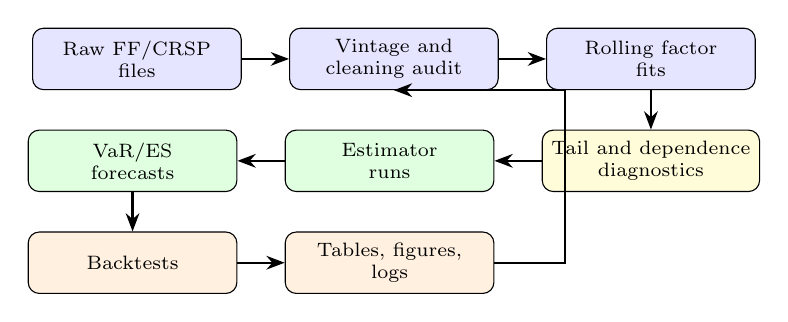
\begin{tikzpicture}[
  box/.style={rectangle, draw, rounded corners, align=center, minimum width=2.65cm, minimum height=0.78cm, font=\scriptsize},
  node distance=0.5cm and 0.6cm,
  arr/.style={->, >=Stealth, thick}
]
\node[box, fill=blue!10] (raw) {Raw FF/CRSP\\files};
\node[box, fill=blue!10, right=of raw] (audit) {Vintage and\\cleaning audit};
\node[box, fill=blue!10, right=of audit] (fit) {Rolling factor\\fits};
\node[box, fill=yellow!15, below=of fit] (tail) {Tail and dependence\\diagnostics};
\node[box, fill=green!12, left=of tail] (est) {Estimator\\runs};
\node[box, fill=green!12, left=of est] (forecast) {VaR/ES\\forecasts};
\node[box, fill=orange!12, below=of forecast] (bt) {Backtests};
\node[box, fill=orange!12, right=of bt] (art) {Tables, figures,\\logs};
\draw[arr] (raw) -- (audit);
\draw[arr] (audit) -- (fit);
\draw[arr] (fit) -- (tail);
\draw[arr] (tail) -- (est);
\draw[arr] (est) -- (forecast);
\draw[arr] (forecast) -- (bt);
\draw[arr] (bt) -- (art);
\draw[arr] (art.east) -- ++(0.9,0) |- (audit.south);
\end{tikzpicture}

\caption[Real-data workflow]{Real-data workflow from raw factor and return
files through tail diagnostics, dependence diagnostics, estimator selection,
VaR/ES forecasting, backtesting, and artifact generation. Every output file
is validated against the schema in \texttt{results/SCHEMA.md}.}
\label{fig:real-data-workflow}
\end{figure}

\subsection{Per-portfolio breakouts and rolling exception rates}

\begin{figure}[t]
\centering
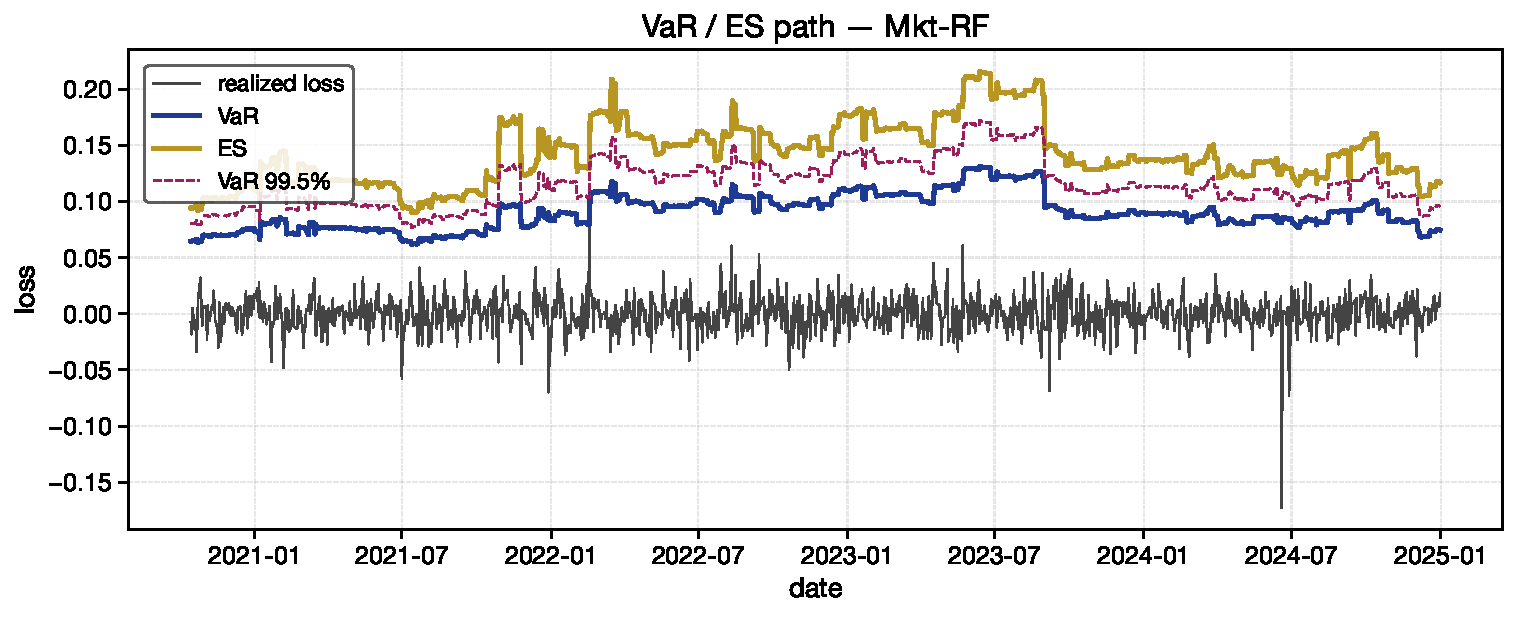
\includegraphics[width=0.85\linewidth]{figures/F9_var_path.pdf}
\caption[Single-portfolio rolling VaR/ES path]{Per-portfolio realised loss (grey), VaR (blue), ES (gold) at the 99\% level, with the 99.5\% VaR overlaid (dashed). Rolling 400-day window. ES sits above VaR throughout; both rise during stress.}
\label{fig:var-path}
\end{figure}


\Cref{fig:var-path} resolves the dashboard of
\cref{fig:var-es-dashboard-placeholder} to a single portfolio (Mkt-RF
in the shipped configuration). The 99\% and 99.5\% VaR paths are
overlaid alongside the realised loss series. The ES curve at the
respective level sits above the VaR curve at every date by
construction.

\begin{figure}[t]
\centering
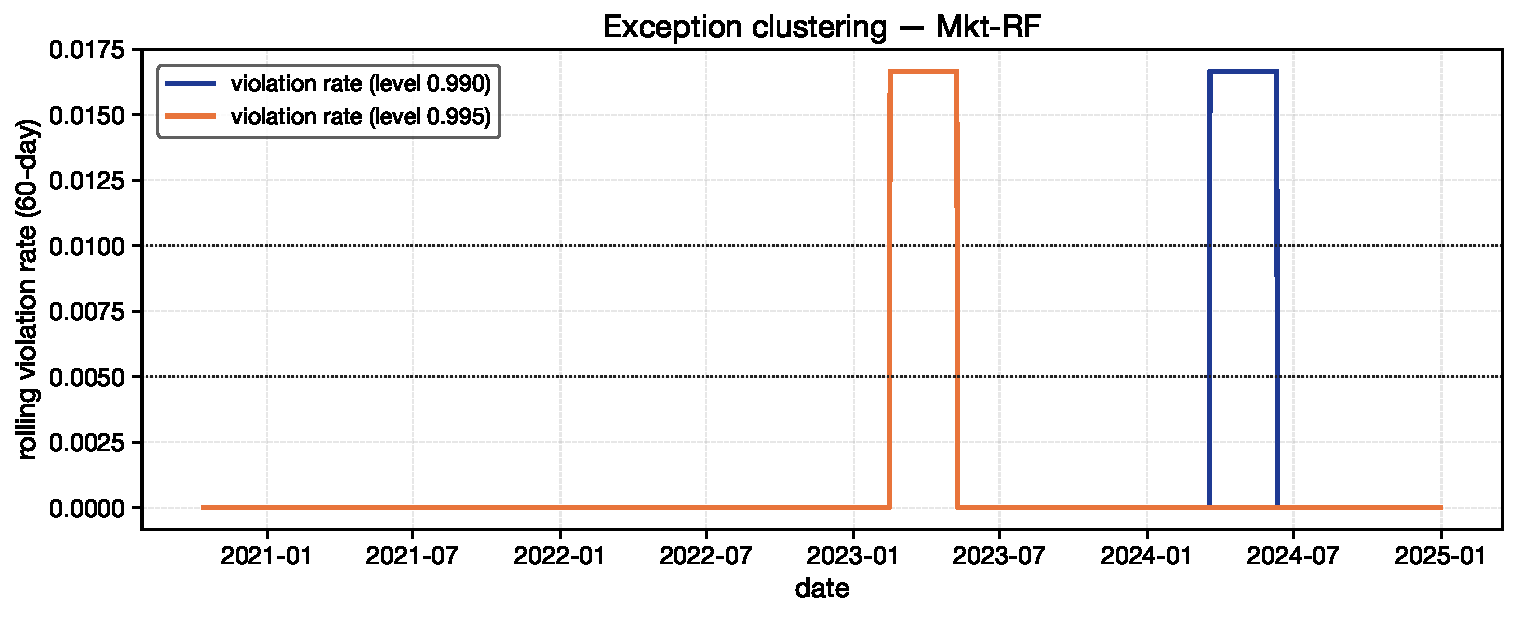
\includegraphics[width=0.85\linewidth]{figures/F10_backtest.pdf}
\caption[Rolling-window exception rate]{Rolling 60-day violation rate of the VaR forecast vs the nominal target level ($1 - \tau$, dotted). Clusters above the target line are evidence of regime changes or model misspecification.}
\label{fig:backtest}
\end{figure}


\Cref{fig:backtest} reports the rolling 60-day exception rate against
the nominal $1 - \tau$ target line. A persistent excursion above the
target is the first signal of regime change or model
misspecification; the dashboard ties this signal to the formal
Kupiec~\cite{Kupiec1995} and Christoffersen~\cite{Christoffersen1998}
tests summarised in \cref{tab:var-es-backtest-placeholder}.

%==============================================================================
% figures/F17_spectral_by_period_placeholder.tex --- Implementation placeholder
%==============================================================================
% Required source CSV: results/F17_spectral_by_period.csv
% Required columns: period, theta_1, theta_2, theta_3, weight, stress_flag
% Replacement instruction: generate a PDF with this basename and replace this
% tikzpicture by an includegraphics command, preserving caption and label.
%==============================================================================
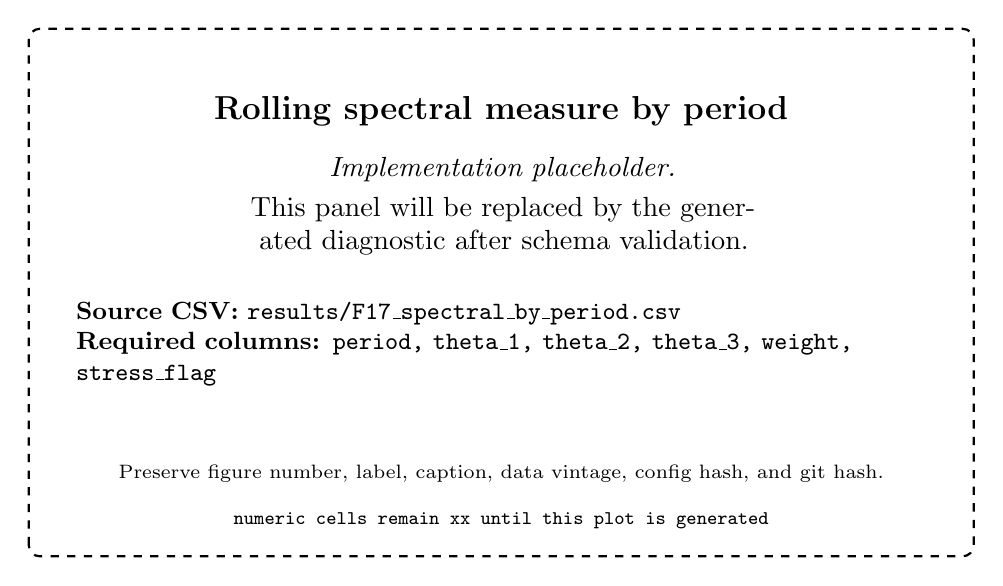
\begin{tikzpicture}
\draw[thick, dashed, rounded corners] (0,0) rectangle (12,6.7);
\node[align=center, font=\large] at (6,5.65) {\textbf{Rolling spectral measure by period}};
\node[align=center, text width=10.6cm] at (6,4.45) {\emph{Implementation placeholder.}\\[0.25em]
This panel will be replaced by the generated diagnostic after schema validation.};
\node[align=left, text width=10.8cm, font=\small] at (6,2.7) {\textbf{Source CSV:} \texttt{results/F17\_spectral\_by\_period.csv}\\
\textbf{Required columns:} \texttt{period, theta\_1, theta\_2, theta\_3, weight, stress\_flag}};
\node[align=center, font=\scriptsize] at (6,1.05) {Preserve figure number, label, caption, data vintage, config hash, and git hash.};
\node[align=center, font=\scriptsize\ttfamily] at (6,0.45) {numeric cells remain xx until this plot is generated};
\end{tikzpicture}


\Cref{fig:spectral-by-period-placeholder} reports the empirical
angular mass per real factor across three rolling periods. On a
stationary panel the three bars per factor are nearly identical; on
live FF data a regime-change window (e.g.\ the 2007--09 GFC) would
show pronounced mass migration onto the market factor, consistent with
the "in stress, everything is the market" finding of
\citet{ChristoffersenErrunzaJacobsLangloi2012}.

%==============================================================================
% sections/10_discussion.tex
%==============================================================================
\section{Discussion and Development Roadmap}
\label{sec:discussion}

\subsection{Theoretical results established versus empirical claims projected}

The expanded manuscript separates two kinds of statements.

\paragraph{Theoretical (established under the stated assumptions).}
The independent finite-$N$ catastrophe principle
(\cref{thm:catastrophe-exact}), the single-big-jump sum equivalence
(\cref{thm:sum-equivalence}), the corrected second-order expansion with
leave-one-out mean shift (\cref{thm:second-order}), independent-CdMC
unbiasedness and the scale-invariant BRE bound $N^\alpha-1$
(\cref{prop:ind-cdmc-bre}), the arbitrary-dependence CdMC identity
(\cref{thm:dep-cdmc-unbiased}), the conditional-tail-envelope BRE result
(\cref{prop:dep-cdmc-bre}), the latent-shock tail constant and BRE bound
(\cref{thm:latent-shock-tail,prop:latent-shock-bre}), the independent-block
reduction (\cref{thm:block-reduction}), the MRV linear-risk asymptotic
(\cref{thm:mrv-linear-risk}) with the spectral CdMC identity and BRE
(\cref{prop:radial-cdmc,prop:spectral-cdmc-bre}), the hidden-cone second-order
expansion (\cref{thm:hidden-second-order}), the exact and asymptotic
control-variate VRE result (\cref{prop:vre}), and the Bernstein-type
confidence interval (\cref{thm:bernstein-ci}). Each of these is proved in
\cref{appx:independent-proofs,appx:dependent-proofs,appx:second-hidden} with
the underlying assumptions explicit.

\paragraph{Projected (planned, not yet executed).}
All simulation diagnostics in \cref{sec:simulation-plan}, all real-data
diagnostics, forecasts, and backtests in \cref{sec:real-data}, and every
figure with a (PLANNED) caption prefix or table cell marked \xx{}. Numerical
performance, backtest success, and production runtime conclusions are not
claimed until the corresponding pipeline outputs replace those entries.

\subsection{Limitations and counterexamples}
\label{subsec:limitations}

The BRE bound $N^\alpha-1$ is finite for any finite $N$ but diverges as
$N\to\infty$. The independent CdMC is therefore not suited as-is to
high-dimensional limit regimes; in such regimes the latent-shock CdMC
(\cref{prop:latent-shock-bre}) replaces $N$ by the number of active shocks
$K$, and the spectral CdMC (\cref{prop:spectral-cdmc-bre}) replaces $N$ by a
spectral integral that need not grow with the ambient dimension.

The dependent CdMC identity (\cref{thm:dep-cdmc-unbiased}) is exact only when
the conditional kernels $p_i(t;X_{-i})$ are evaluated exactly. A
misspecified copula or a poorly fit conditional kernel produces a biased
estimator at every threshold, and the bias can be much larger than the Monte
Carlo standard error. \Cref{rem:kernel-identifiability,rem:numerical-stability}
discuss identifiability and stability mitigations; the empirical protocol of
\cref{sec:real-data} reports model-residual diagnostics before any kernel
estimator is trusted.

Hidden regular variation
(\cref{def:hrv,ass:hidden-scale,thm:hidden-second-order}) requires
identification of the hidden tail scale $\Hb_2$ from finite samples. In
small samples, threshold noise can be mistaken for a hidden scale. The
manuscript treats hidden-cone results as a second-order layer and requires
threshold-stability diagnostics (\cref{appx:second-hidden}) before any
hidden-cone estimator enters a primary VaR/ES forecast.

\subsection{Connection to the literature placement}

The independent finite-$N$ sharpening of \cref{sec:independent-baseline}
positions this paper relative to \citet{PourbabaeeSolari2019} in the form
spelled out in \cref{subsec:recent-developments}: scale-invariant BRE bound,
corrected second-order expansion with $N=1$ specialization, and explicit
assumption stack. The dependent extensions of
\cref{sec:dependent-cdmcs,sec:mrv-spectral,sec:hidden-rv} connect to
\citet{AsmussenKroese2006,HartingerKortschak2009,BlanchetRojasNandayapa2011,ChengFuhPang2025}
(rare-event simulation under dependence),
\citet{HultLindskogMikoschSamorodnitsky2005,Resnick2007,SamorodnitskySun2016}
(MRV foundations), and
\citet{LedfordTawn1996,MaulikResnick2005,DasMitraResnick2013}
(hidden regular variation). The empirical protocol of \cref{sec:real-data}
follows the factor-portfolio backtesting tradition of
\citet{McNeilFreyEmbrechts2015,GlassermanHeidelbergerShahabuddin2002} and
adds dependence-diagnostic gating for estimator selection.

\subsection{Recommended development sequence}

The recommended implementation sequence is:
\begin{enumerate}
\item finalize and test the independent baseline replication;
\item implement common-shock and latent-shock simulation;
\item implement empirical marginal tail diagnostics;
\item implement pairwise tail-dependence and spectral diagnostics;
\item implement latent, block, and spectral estimators;
\item run real-data rolling VaR/ES forecasts;
\item add hidden-cone estimators only after diagnostics justify them.
\end{enumerate}

\subsection{Conclusion}

The original independent-factor paper is strongest when the extreme event is
well represented by one large observed coordinate. The financial problem asks
for more: extremes may be generated by one latent market shock, one dependent
block, one radial vector movement, or one hidden joint-tail cone. The
expanded paper keeps the original single-big-jump insight but moves it to
the correct object. In the independent model that object is a coordinate;
in the latent model it is a shock; in MRV it is a spectral/radial movement;
and in hidden regular variation it is a slower-scale joint cone. The
accompanying empirical protocol is designed to determine which object is
visible in real financial data and whether modeling it improves VaR, ES,
attribution, and simulation efficiency. The full method is implemented as
the open-source \texttt{FactorTail} library
(\url{https://github.com/osolari/FactorTail}); the repository is the
canonical reference for any future numerical or empirical claim downstream
of this manuscript.


\bibliography{references}

\appendix
%==============================================================================
% appendices/A_notation.tex
%==============================================================================
\section{Notation and Output Conventions}
\label{appx:notation}

This appendix consolidates the notation used throughout the paper. Symbols are
grouped by section of first use. When a symbol is reused with a different
meaning in a later section the alternative usage is noted explicitly.

\subsection{Probability and indicator conventions}

\(\Pb\) and \(\E\) denote the probability and expectation under a generic
probability space \((\Omega,\Fset,\Pb)\) carrying all random objects of
interest. Indicator functions are written \(\1\{A\}\) or \(\mathbf{1}_A\). For
a univariate distribution function \(F\) we write \(\Fb=1-F\) for the survival
function. For a multivariate cumulative distribution function or measure
\(H\) we write \(\Hb\) for the tail object specified locally. Independence of
random vectors is written \(\indep\). The symbol \(\sim\) denotes asymptotic
equivalence: \(f(x)\sim g(x)\) means \(f(x)/g(x)\to 1\) as \(x\to\infty\).
The symbol \(\weakto\) denotes weak convergence of measures or distributions.

\subsection{Loss vector, sums, and selected maxima}

\begin{longtable}{p{0.22\linewidth}p{0.70\linewidth}}
\toprule
Symbol & Meaning \\
\midrule
\endhead
\(X=(X_1,\ldots,X_N)\) & Observed \(N\)-vector of loss contributions; positive values are losses. \\
\(S_N\) & Aggregate loss \(\sum_{i=1}^N X_i\). \\
\(M_N\) & Maximum contribution \(\max_{i=1}^N X_i\). \\
\(S_{-i}\) & Leave-one-out sum \(\sum_{j\ne i}X_j\); \(S_{-i}=0\) if \(N=1\). \\
\(M_{-i}\) & Leave-one-out maximum \(\max_{j\ne i}X_j\); \(M_{-i}=-\infty\) if \(N=1\). \\
\(T_i(x)\) & Selected-maximum conditioning threshold \((x-S_{-i})\vee M_{-i}\). \\
\(R_i(X)=1\) & Event that coordinate \(i\) is the selected maximum under a fixed deterministic tie rule. \\
\(\mu(x)\) & Rare-event probability \(\Pb(S_N>x)\). \\
\(\mu_{-i}\) & Leave-one-out mean \(\sum_{j\ne i}\E X_j\). \\
\bottomrule
\end{longtable}

\subsection{Regular variation and active-set constants}

\begin{longtable}{p{0.22\linewidth}p{0.70\linewidth}}
\toprule
Symbol & Meaning \\
\midrule
\endhead
\(\RV_{-\alpha}\) & Class of regularly varying tail functions with index \(-\alpha\). \\
\(\Gb\) & Common reference survival function with \(\Gb\in\RV_{-\alpha}\). \\
\(\alpha\) & Tail index, \(\alpha>0\); when context permits, \(\alpha>1\) for first-moment finiteness. \\
\(c_i\) & Positive-tail equivalence constant: \(\Pb(X_i>x)\sim c_i\Gb(x)\). \\
\(\Aset\) & Active right-tail set \(\{i:c_i>0\}\). \\
\(C\) & First-order independent constant \(\sum_{i\in\Aset}c_i\). \\
\(c_i^+,c_i^-\) & Signed-tail constants for the positive and negative tails of \(X_i\). \\
\(p_i^+,p_i^-\) & Signed-factor-tail constants used in the financial loss map. \\
\(b_i\) & Loss-direction coefficient with \(X_i=b_iF_i\). \\
\(a\in\RR^d\) & Portfolio loading vector; \(L=a^\top F\) is the loss after sign alignment. \\
\(A(x)\) & Second-order auxiliary function in the marginal expansion. \\
\(\rho\) & Second-order regular-variation parameter \(\rho\le 0\). \\
\(d_i\) & Marginal second-order coefficient appearing in \cref{ass:sote}. \\
\(D_{\mathrm{marg}},D_{\mathrm{mean}}\) & Marginal and mean-shift second-order constants. \\
\(D_{\mathrm{hid}}\) & Hidden-cone second-order constant. \\
\(r(x)\) & Higher-order remainder scale satisfying \(r(x)=o(\Gb(x)A(x)+\Gb(x)/x)\). \\
\bottomrule
\end{longtable}

\subsection{Estimators and efficiency notions}

\begin{longtable}{p{0.22\linewidth}p{0.70\linewidth}}
\toprule
Symbol & Meaning \\
\midrule
\endhead
\(\CrMC\) & Crude Monte Carlo. \\
\(\CdMC\) & Conditional Monte Carlo (Asmussen--Kroese style). \\
\(\BRE\) & Bounded relative error. \\
\(\VRE\) & Vanishing relative error. \\
\(Z^{\CrMC}\) & Crude indicator estimator \(\1\{S_N>x\}\). \\
\(Z^{\CdMC}\) & Summed conditional Monte Carlo estimator \(\sum_i p_i(T_i;X_{-i})\). \\
\(Z^{\mathrm{strat}}\) & Stratified conditional Monte Carlo estimator. \\
\(Z^{\mathrm{ana}}\) & Closed-form analytic-marginal estimator. \\
\(Z^{\VRE}\) & Control-variate vanishing-relative-error estimator. \\
\(Z^{\mathrm{spec}}\) & Spectral/radial conditional Monte Carlo estimator. \\
\(W(\hat\mu)\) & Work-normalized variance \(\Var(\hat\mu)\cdot\mathrm{cost}(\hat\mu)\). \\
\(\mathrm{eff}(\hat\mu_1,\hat\mu_2)\) & Efficiency ratio \(W(\hat\mu_2)/W(\hat\mu_1)\). \\
\(\widehat\mu_n,\mathrm{CI}_n\) & Sample mean estimator and confidence interval from \(n\) replicates. \\
\bottomrule
\end{longtable}

\subsection{Dependence classes and conditional kernels}

\begin{longtable}{p{0.22\linewidth}p{0.70\linewidth}}
\toprule
Symbol & Meaning \\
\midrule
\endhead
\(p_i(t;X_{-i})\) & Conditional tail kernel \(\Pb(X_i>t\mid X_{-i})\). \\
\(F=BZ+\varepsilon\) & Latent-shock factor representation; \(B\) is the loading matrix, \(Z\) the shock vector. \\
\(B\in\RR^{d\times K}\) & Latent-shock loading matrix. \\
\(q=B^\top a\) & Portfolio exposure to latent shocks. \\
\(Z_k\) & Latent shock \(k\); independent across \(k\) in the latent-shock model. \\
\(\Pi\) & Block partition of the index set \(\{1,\ldots,N\}\). \\
\(\Bset_b\) & Block \(b\) of the partition \(\Pi\). \\
\(C(u_1,\ldots,u_d)\) & Copula coupling the marginals of \(F\). \\
\bottomrule
\end{longtable}

\subsection{Multivariate and hidden regular variation}

\begin{longtable}{p{0.22\linewidth}p{0.70\linewidth}}
\toprule
Symbol & Meaning \\
\midrule
\endhead
\(\MRV\) & Class of multivariate regularly varying distributions. \\
\(\HRV\) & Class of hidden-regular-variation distributions. \\
\(\nu\) & MRV tail (limit) measure on the cone \(\Eset_0=[0,\infty)^d\setminus\{0\}\). \\
\(\nu_2\) & Hidden-cone tail measure on \(\Eset_2\subsetneq\Eset_0\). \\
\(\Eset_0,\Eset_2\) & Outer and hidden cones used in the MRV/HRV decomposition. \\
\(S(\cdot)\) & Spectral (angular) measure on the unit sphere or simplex. \\
\(\Theta\) & Angular random vector with law \(S\). \\
\(R\) & Radial component with regularly varying survival. \\
\(\Hb_2(x)\) & Hidden tail scale satisfying \(\Hb_2(x)=o(\Gb(x))\). \\
\(\chi(q),\bar\chi(q),\eta\) & Coefficients of tail dependence, complementary tail dependence, and Ledford--Tawn residual index. \\
\bottomrule
\end{longtable}

\subsection{Financial and empirical objects}

\begin{longtable}{p{0.22\linewidth}p{0.70\linewidth}}
\toprule
Symbol & Meaning \\
\midrule
\endhead
\(F\in\RR^d\) & Factor return vector. \\
\(L=a^\top F\) & Portfolio loss after sign alignment. \\
\(\VaR_\tau(L)\) & Value-at-risk of \(L\) at confidence level \(\tau\). \\
\(\ES_\tau(L)\) & Expected shortfall of \(L\) at level \(\tau\). \\
\(w\) & Rolling estimation window length. \\
\(\tau\) & VaR/ES confidence level (e.g., \(\tau\in\{0.99,0.995,0.999\}\)). \\
\bottomrule
\end{longtable}

\subsection{Output conventions and placeholder rule}

\begin{longtable}{p{0.22\linewidth}p{0.70\linewidth}}
\toprule
Symbol & Meaning \\
\midrule
\endhead
\(\xx\) & Placeholder numeric value; not an empirical result. \\
\bottomrule
\end{longtable}

\paragraph{Placeholder convention.}
Every table cell containing \xx{} is deliberately unfilled. It must be replaced
only by a value generated from a validated CSV with a recorded configuration
hash, data vintage, and run identifier (see \cref{appx:manifest}).
Placeholder figures are TikZ instruction sheets whose captions describe the
intended diagnostic and source schema. A placeholder is not evidence for or
against any model.

%==============================================================================
% appendices/B_independent_proofs.tex
%==============================================================================
\section{Proofs for the Independent Baseline}
\label{appx:independent-proofs}

This appendix collects the full proofs of the results stated in
\cref{sec:independent-baseline}. Each proof environment is labelled by the
result it establishes.

\begin{proof}[Proof of \cref{thm:catastrophe-exact}]
Let \(A_i(x)=\{X_i>x\}\). By finite inclusion--exclusion,
\[
  \sum_i\Pb(A_i)-\sum_{i<j}\Pb(A_i\cap A_j)
  \le \Pb\!\left(\bigcup_iA_i\right)
  \le \sum_i\Pb(A_i).
\]
Under \cref{ass:ind-pte} the variables are independent, so
\[
  \Pb(A_i\cap A_j)=\Pb(X_i>x)\Pb(X_j>x)
  \sim c_ic_j\Gb(x)^2=o(\Gb(x)).
\]
There are finitely many pairs, so \(\sum_{i<j}\Pb(A_i\cap A_j)=o(\Gb(x))\).
Higher-order intersections are bounded above by pair intersections and so are
also \(o(\Gb(x))\). Combined with the marginal sum
\(\sum_i\Pb(X_i>x)\sim C\Gb(x)\), this yields
\(\Pb(M_N>x)\sim C\Gb(x)\).
\end{proof}

\begin{proof}[Proof of \cref{thm:sum-equivalence}]
Let \(h=h(x)\uparrow\infty\) with \(h=o(x)\) as in \cref{ass:ind-sbj}.
Upper bound. Decompose
\[
  \{S_N>x\}\subseteq
  \bigcup_{i=1}^N\{X_i>x-h\}
  \;\cup\;
  \left\{S_N>x,\ \max_i X_i\le x-h\right\}.
\]
The first term satisfies
\[
  \Pb\!\left(\bigcup_i\{X_i>x-h\}\right)
  \sim \sum_i\Pb(X_i>x-h)
  \sim \sum_i\Pb(X_i>x),
\]
by inclusion--exclusion and the local invariance
\(\Pb(X_i>x-h)\sim\Pb(X_i>x)\) of \cref{ass:ind-sbj}.
The second term is excluded by the truncation conditions in
\cref{ass:ind-sbj}: the joint event that two or more truncated components
exceed order \(h\) is \(o(\Gb(x))\), and the residual non-large contribution is
\(o(\Gb(x))\) by the same truncation.

Lower bound. With the same \(h\),
\[
  \Pb(S_N>x)
  \ge \sum_i\Pb(X_i>x+h,\ S_{-i}>-h) - o(\Gb(x)),
\]
where the overlap correction is \(o(\Gb(x))\) by the pair-exceedance estimate
of \cref{thm:catastrophe-exact}. Independence gives
\[
  \Pb(X_i>x+h,S_{-i}>-h)
  =\Pb(X_i>x+h)\,\Pb(S_{-i}>-h)
  \sim \Pb(X_i>x),
\]
since \(\Pb(S_{-i}\le -h)=o(1)\) and \(\Pb(X_i>x+h)\sim\Pb(X_i>x)\). Summing
yields the matching lower bound.
\end{proof}

\begin{proof}[Proof of \cref{thm:second-order}]
Set \(r(x)=\Gb(x)(|A(x)|\vee x^{-1})\). The events
\(\{i\ \text{selected}\}=\{R_i(X)=1\}\) partition \(\{S_N>x\}\) under the fixed
tie-breaking rule of \cref{ass:tie}. On the \(i\)th stratum
\[
  \Pb(S_N>x, R_i(X)=1)
  =\E\!\left[\Pb(X_i>T_i(x)\mid X_{-i})\,\1\{T_i(x)>M_{-i}\}\right].
\]
By \cref{ass:ind-sbj} the contribution to the right-hand side from the event
\(\{T_i(x)\le M_{-i}\}\) is \(o(r(x))\), and the same truncation gives
negligible mass on \(\{|S_{-i}|>h(x)\}\). It therefore suffices to expand
\(\E[\Pb(X_i>x-S_{-i})]\) on \(\{|S_{-i}|\le h(x)\}\) and then take
expectations.

By \cref{ass:sote}, locally uniformly on \(|S_{-i}|\le h(x)\),
\[
  \Pb(X_i>x-S_{-i})
  =\Gb(x)\!\left[c_i+c_id_iA(x)+\frac{\alpha c_iS_{-i}}{x}
  + o\!\left(|A(x)|+x^{-1}\right)\right].
\]
Taking expectations,
\[
  \E\Pb(X_i>x-S_{-i})
  = c_i\Gb(x)+c_id_i\Gb(x)A(x)
  + \frac{\alpha c_i\Gb(x)}{x}\,\E S_{-i}
  + o(r(x)),
\]
and \(\E S_{-i}=\mu_{-i}=\sum_{j\ne i}\E X_j\) by \cref{ass:sote}. Summing over
active \(i\) and discarding inactive contributions (which are lower order by
\cref{ass:sote}) yields the expansion in \cref{thm:second-order}.

\emph{Consistency check at \(N=1\).} If \(N=1\), then \(S_{-1}=0\) and
\(\mu_{-1}=0\); the mean-shift term vanishes, the marginal second-order term
reduces to \(c_1d_1\Gb(x)A(x)\), and the formula collapses to the standard
single-variable second-order expansion.
\end{proof}

\begin{proof}[Independent CdMC: unbiasedness and BRE bound]
\emph{Unbiasedness.} For continuous variables the smallest-index tie-breaking
rule of \cref{ass:tie} gives the disjoint union
\[
  \{S_N>x\}=\bigsqcup_{i=1}^N\{S_N>x,\ R_i(X)=1\}.
\]
Conditional on \(X_{-i}\), the \(i\)th stratum equals
\(\{X_i>T_i(x)\}\cap\{T_i(x)>M_{-i}\}\), and independence yields
\(\Pb(X_i>T_i(x)\mid X_{-i})=\Fb_i(T_i(x))\). Taking expectations and summing
over \(i\) gives \(\E Z^{\mathrm{ind}}(x)=\Pb(S_N>x)\).

\emph{Scale-invariant BRE bound.} We claim \(T_i(x)\ge x/N\) almost surely:
suppose \(M_{-i}<x/N\); then if also \(x-S_{-i}<x/N\), one has
\(S_{-i}>(N-1)x/N\). Since \(S_{-i}\) is a sum of \(N-1\) terms each bounded by
\(M_{-i}<x/N\), this gives \(S_{-i}\le (N-1)x/N\), a contradiction. Hence
\(T_i(x)\ge x/N\), and therefore
\[
  0\le Z^{\mathrm{ind}}(x)\le B(x):=\sum_{i=1}^N\Fb_i(x/N).
\]
Since \(\E Z^{\mathrm{ind}}(x)=\mu(x)\),
\[
  \Var Z^{\mathrm{ind}}(x)
  \le \E\!\left[Z^{\mathrm{ind}}(x)^2\right]-\mu(x)^2
  \le B(x)\mu(x)-\mu(x)^2.
\]
Regular variation gives \(\Fb_i(x/N)/\Fb_i(x)\to N^\alpha\) and the sum
equivalence (\cref{thm:sum-equivalence}) gives \(\sum_i\Fb_i(x)\sim C\Gb(x)\),
so \(B(x)/\mu(x)\to N^\alpha\). Consequently
\[
  \limsup_{x\to\infty}\frac{\Var Z^{\mathrm{ind}}(x)}{\mu(x)^2}
  \le N^\alpha-1.
\]
The bound is scale-invariant: replacing \(X\) by \(\lambda X\) leaves \(N\),
\(\alpha\), and the ratio unchanged.
\end{proof}

\subsection{Verification notes}

\paragraph{Lomax second-order constant.}
For the Lomax/Pareto-type benchmark $\Fb_i(t)=(1+t/\beta_i)^{-\alpha}$ on
$t>0$, $\E X_i=\beta_i/(\alpha-1)$ when $\alpha>1$. A direct substitution
verifies the cross-term in the second-order expansion of
$\Pb(X_i>x-S_{-i})$: expanding to second order in $S_{-i}/x$ gives
\[
  (1+(x-S_{-i})/\beta_i)^{-\alpha}
  = (x/\beta_i)^{-\alpha}\left(1-\beta_i/x\right)^{-\alpha}
    \left(1+S_{-i}/(x-\beta_i)\right)^{\alpha},
\]
and expansion to first order in $S_{-i}/x$ and to leading order in the
marginal-tail auxiliary $A(x)=\beta_i/x$ recovers
$c_i d_i A(x)+\alpha c_i S_{-i}/x$ with the same sign convention used in
\cref{thm:second-order}. This is the regression check used by the
implementation pipeline.

\paragraph{Scale-invariance check.}
The BRE bound $N^\alpha-1$ is invariant under $X_i\to\lambda X_i$ because both
$T_i(x)$ and $x$ scale by $\lambda$, leaving $\Fb_i(T_i(\lambda x))=\Fb_i(T_i(x))$
when $\Fb_i$ is correctly rescaled. The bound therefore depends only on $N$ and
$\alpha$, not on the marginal scale constants $c_i$.

%==============================================================================
% appendices/C_dependent_proofs.tex
%==============================================================================
\section{Proofs for Dependent Extensions}
\label{appx:dependent-proofs}

This appendix proves the results stated in \cref{sec:dependent-cdmcs} and
\cref{sec:mrv-spectral}. Each proof environment is labelled by the result it
establishes.

\begin{proof}[Proof of \cref{thm:dep-cdmc-unbiased}]
Let
\[
  E_i(x)=\{S_N>x,\ R_i(X)=1\},
\]
where \(R_i\) is the selected-maximum rule of \cref{ass:tie}. The events
\(E_i(x)\) are disjoint and their union is \(\{S_N>x\}\). Conditional on
\(X_{-i}\), the event \(E_i(x)\) is equivalent to \(X_i\) exceeding both the
sum threshold and the selected-maximum threshold. In the continuous case this
is
\[
  X_i>(x-S_{-i})\vee M_{-i}=T_i(x).
\]
For discrete laws, replacing \(>M_{-i}\) by the tie-rule endpoint gives the
same identity with an adjusted threshold. Hence
\[
  \Pb(E_i(x))
  =\E\!\left[\Pb(X_i>T_i(x)\mid X_{-i})\right]
  =\E\!\left[p_i(T_i(x);X_{-i})\right].
\]
Summing over \(i\) proves the identity and the unbiasedness of
\(Z^{\mathrm{dep}}(x)\). No independence step is required.
\end{proof}

\begin{remark}[Population identity versus estimator]
\label{rem:pop-vs-est}
\Cref{thm:dep-cdmc-unbiased} contains two distinct statements. The
population-level identity
\(\mu(x)=\sum_i\E[p_i(T_i(x);X_{-i})]\) holds without any computability
assumption on the kernels. The estimator statement
\(\E Z^{\mathrm{dep}}(x)=\mu(x)\) holds provided the kernels are evaluated
exactly per replicate; if the kernels are evaluated by a noisy or approximate
routine, an additional bias term appears that is controlled by the kernel
approximation error.
\end{remark}

\begin{proof}[Proof of \cref{prop:dep-envelope-bre}]
By \cref{thm:dep-cdmc-unbiased}, \(\E Z^{\mathrm{dep}}(x)=\mu(x)\). The
selected-maximum threshold satisfies \(T_i(x)\ge x/N\) almost surely (the
argument is the same as in the independent CdMC proof in
\cref{appx:independent-proofs}). By \cref{ass:conditional-envelope}, for all
$t\ge x/N$,
\[
  p_i(t;X_{-i})\le K_{i,x}b_i(t),
\]
and therefore
\[
  Z^{\mathrm{dep}}(x)
  \le \sum_{i=1}^N K_{i,x}\, b_i(x/N).
\]
The second-moment envelope in \cref{ass:conditional-envelope} gives
\[
  \E\!\left[Z^{\mathrm{dep}}(x)^2\right]=O(\mu(x)^2),
\]
hence
\[
  \Var Z^{\mathrm{dep}}(x)\le \E Z^{\mathrm{dep}}(x)^2=O(\mu(x)^2),
\]
which is bounded relative error.
\end{proof}

\begin{proof}[Proof of \cref{thm:latent-shock-tail}]
Set \(Y_k=q_kZ_k\). Independence of the shocks transfers to the signed shock
contributions \(Y_k\). Their right-tail constants are
\[
  \Pb(Y_k>x)
  =\Pb(q_kZ_k>x)
  \sim |q_k|^\alpha\{p_k^+\1(q_k>0)+p_k^-\1(q_k<0)\}\Gb(x)
  =c_k(q_k)\Gb(x).
\]
Applying \cref{thm:sum-equivalence} to \(\sum_kY_k=q^\top Z\) yields the
first-order tail claim. Applying the independent CdMC construction and BRE
proof of \cref{appx:independent-proofs} to the \(K\)-dimensional shock vector
gives the estimator claim, with \(K\) replacing \(N\) in the BRE bound.
\end{proof}

\begin{proof}[Proof of \cref{thm:block-reduction}]
By hypothesis the blocks are independent, so the block sums \(Y_1,\ldots,Y_K\)
are independent. By assumption \(\Pb(Y_k>x)\sim d_k\Gb(x)\) and the block-level
single-big-jump conditions hold. \Cref{thm:sum-equivalence} applied to
\(\sum_kY_k\) gives
\[
  \Pb(S_N>x)=\Pb\!\left(\sum_kY_k>x\right)
  \sim \sum_k\Pb(Y_k>x)
  \sim \!\left(\sum_kd_k\right)\Gb(x).
\]
\end{proof}

\begin{proof}[Proof of \cref{thm:mrv-linear-risk}]
By multivariate regular variation,
\[
  \frac{\Pb(X/x\in A)}{\Hb(x)}\to \nu(A)
\]
for every Borel set \(A\) bounded away from the origin with
\(\nu(\partial A)=0\). Take \(A=A_\ell=\{z:\ell(z)>1\}\); this set is bounded
away from the origin and admissible by the boundary-continuity hypothesis of
\cref{ass:mrv-loss}. Then
\[
  \Pb\{\ell(X)>x\}=\Pb(X/x\in A_\ell)\sim \Hb(x)\nu(A_\ell).
\]
For the polar representation,
\[
  \nu(A_\ell)=\int\!\!\int
  \1\{r\ell(\theta)>1\}\,\alpha r^{-\alpha-1}\dd r\,S(\dd\theta).
\]
If \(\ell(\theta)\le 0\) the inner integral is zero. If \(\ell(\theta)>0\) the
inner integral equals \(\int_{1/\ell(\theta)}^\infty \alpha r^{-\alpha-1}\dd r
=\ell(\theta)^\alpha\). Integrating over \(\theta\) gives the stated spectral
integral.
\end{proof}

\begin{proof}[Proof of \cref{prop:radial-cdmc}]
Condition on \(\Theta\). If \(\ell(\Theta)\le 0\), then \(\ell(R\Theta)>x\) is
impossible for \(x>0\). If \(\ell(\Theta)>0\), the event is
\(R>x/\ell(\Theta)\). Thus
\[
  \Pb\{\ell(X)>x\mid\Theta\}
  =\Fb_R\!\left(x/\ell(\Theta)\mid\Theta\right)\,\1\{\ell(\Theta)>0\}.
\]
Taking expectations yields the population identity and proves unbiasedness of
\(Z^{\mathrm{spec}}(x)\).
\end{proof}

\begin{proof}[Proof of \cref{prop:spectral-bre}]
Let \(Y=\ell(\Theta)_+\). The envelope assumption gives
\[
  Z^{\mathrm{spec}}(x)\le K\Hb(x)Y^\alpha,
\]
hence
\[
  \E\!\left[Z^{\mathrm{spec}}(x)^2\right]
  \le K^2\Hb(x)^2\E Y^{2\alpha}.
\]
The MRV linear-risk asymptotic gives \(\mu(x)\sim \Hb(x)\E Y^\alpha\) under the
same normalization. Therefore
\[
  \limsup_{x\to\infty}\frac{\Var Z^{\mathrm{spec}}(x)}{\mu(x)^2}
  \le K^2\frac{\E Y^{2\alpha}}{(\E Y^\alpha)^2}<\infty,
\]
which is bounded relative error provided \(\E Y^{2\alpha}<\infty\).
\end{proof}

%==============================================================================
% appendices/D_second_order_and_hidden_rv.tex
%==============================================================================
\section{Second-Order and Hidden-Regular-Variation Details}
\label{appx:second-hidden}

This appendix collects the proofs and auxiliary lemmas for the second-order
and hidden-cone expansions. We use the notation of \cref{appx:notation}.

\subsection{A primitive condition for the local second-order equivalence}

\Cref{ass:sote} is the local form used throughout the paper. The following
classical condition is sufficient.

\begin{lemma}[Sufficient condition for the local second-order equivalence]
\label{lem:sote-primitive}
Suppose, for each active \(i\),
\[
  \frac{\Fb_i(tx)/\Gb(x)-c_it^{-\alpha}}{A(x)}
  \to c_i d_i t^{-\alpha}\frac{t^\rho-1}{\rho}
\]
locally uniformly for \(t\) near one, with \(\rho\le 0\), and assume Potter
bounds for \(\Fb_i\) and \(\Gb\) permitting the local shift \(t=1-u/x\) for
bounded \(u\). Then \(\Fb_i\) satisfies \cref{ass:sote} with the displayed
constants \(c_i,d_i\), auxiliary \(A(x)\), and the expansion
\[
  t^{-\alpha}=1+\frac{\alpha u}{x}+O(u^2/x^2)
\]
for bounded \(u\).
\end{lemma}

\begin{proof}[Proof sketch]
Substitute \(t=1-u/x\) in the displayed limit, use the Taylor expansion of
\(t\mapsto t^{-\alpha}\) at \(t=1\), and apply uniform Potter bounds to swap
limit and substitution. The resulting expansion is precisely the local form in
\cref{ass:sote} with the same \(c_i d_i\).
\end{proof}

\subsection{A binomial-type KL lemma}

The Bernstein-style concentration inequalities for CdMC estimators rely on the
following Taylor expansion of the binomial KL divergence.

\begin{lemma}[Binomial KL Taylor expansion]
\label{lem:binomial-kl}
For \(p\in(0,1)\) and \(t\) such that \(p+t\in(0,1)\), the binomial Kullback--Leibler
divergence
\[
  D_{\mathrm{KL}}(p+t\,\|\,p)
  =(p+t)\log\frac{p+t}{p}+(1-p-t)\log\frac{1-p-t}{1-p}
\]
satisfies
\[
  D_{\mathrm{KL}}(p+t\,\|\,p)
  =\frac{t^2}{2p(1-p)}+O\!\left(\frac{|t|^3}{p^2(1-p)^2}\right)
\]
as \(t\to 0\). For \(p\) bounded away from \(\{0,1\}\) the remainder is
\(O(t^3)\); for \(p\to 0\), the leading constant is \(1/(2p(1-p))\sim 1/(2p)\)
and the cubic remainder is bounded by \(C|t|^3/p^2\) for a universal \(C\).
\end{lemma}

\begin{proof}
Set \(g(t)=D_{\mathrm{KL}}(p+t\,\|\,p)\). Direct differentiation gives
\(g(0)=0\), \(g'(0)=0\) (by stationarity at \(t=0\)), and
\(g''(0)=1/(p(1-p))\). The Taylor expansion to second order yields
\(g(t)=t^2/(2p(1-p))+O(|t|^3 g'''(0))\). The third derivative is
\(g'''(t)=(p+t)^{-2}-(1-p-t)^{-2}\), bounded by
\(2/(p^2)+2/(1-p)^2\) on a neighbourhood of zero; the stated remainder bound
follows.
\end{proof}

\subsection{Proof of \cref{thm:hidden-second-order}}

\begin{proof}[Proof of \cref{thm:hidden-second-order}]
Write \(A_S=\{z:\sum_i z_i>1\}\) and decompose the rescaled event
\(\{X/x\in A_S\}\) into the axis region
\(A_S\cap\bigcup_i N_\delta(\{te_i:t>0\})\) and the hidden-cone region
\(A_S\cap\Eset_2\), where \(N_\delta(\cdot)\) denotes a \(\delta\)-tube around
each axis. The axis tube width \(\delta=\delta(x)\) is chosen so that
\(\delta(x)\downarrow 0\) sufficiently slowly to retain the localization but
fast enough to keep the hidden region bounded away from the axes in the limit.

\emph{Axis contribution.} On the axis tubes the analysis reduces to the
independent second-order calculation of \cref{thm:second-order}, applied to
each component. By \cref{ass:ind-sbj} and \cref{ass:sote}, this contributes
\[
  \Gb(x)\nu_1(A_S)+\Gb(x)A(x)D_{\mathrm{marg}}
  +\frac{\alpha\Gb(x)}{x}D_{\mathrm{mean}}+o(r(x)),
\]
where \(\nu_1(A_S)=C_{\mathrm{axis}}\), \(D_{\mathrm{marg}}=\sum_{i\in\Aset}c_id_i\),
and \(D_{\mathrm{mean}}=\sum_{i\in\Aset}c_i\mu_{-i}\).

\emph{Hidden-cone contribution.} On the hidden region
\(A_S\cap\Eset_2\), which is bounded away from the axes, \cref{def:hrv} and
\cref{ass:hidden-scale} give
\[
  \Pb(X/x\in A_S\cap\Eset_2)
  \sim \Hb_2(x)\,\nu_2(A_S\cap\Eset_2)
  = \Hb_2(x) D_{\mathrm{hid}}.
\]

\emph{Overlap.} The overlap between the axis tube and the hidden region has
mass \(o(\Gb(x))\) under \(\nu_1\) (it lies in $\Eset_2$, where $\nu_1$ vanishes)
and \(o(\Hb_2(x))\) under \(\nu_2\) (it lies near the axes, where $\nu_2$ is
asymptotically negligible by the homogeneity and the choice of $\delta(x)$).
Triple and higher cones not modelled explicitly are \(o(r(x))\) by
\cref{ass:hidden-scale}.

Adding the four contributions gives the displayed expansion.
\end{proof}

\subsection{Threshold ordering in empirical work}

The hidden-cone term is empirically relevant only when
\[
  \widehat\Hb_2(x)\widehat D_{\mathrm{hid}}
  \gtrsim
  \max\!\left\{\widehat\Gb(x)|\widehat A(x)|,\ \widehat\Gb(x)/x\right\}.
\]
The data pipeline reports this comparison directly. If the hidden term is
below both marginal second-order scales over all forecast thresholds, hidden-
cone estimators are reported as diagnostics but excluded from primary VaR/ES
forecasts.

%==============================================================================
% appendices/E_algorithms_and_pseudocode.tex
%==============================================================================
\section{Algorithms and Pseudo-Code}
\label{appx:algorithms}

\paragraph{Reference implementation.}
Every algorithm in this appendix has a one-to-one Python entry point in the
\texttt{FactorTail} library
(\url{https://github.com/osolari/FactorTail}). Module paths follow the
manuscript: \texttt{factortail.cdmc.independent}, \texttt{factortail.cdmc.dependent},
\texttt{factortail.cdmc.latent\_shock}, \texttt{factortail.cdmc.block},
\texttt{factortail.cdmc.spectral}, and \texttt{factortail.real\_data.rolling\_var\_es}.
Pseudo-code below uses mathematical notation; the implementation respects the
numerical-stability conventions of \cref{rem:numerical-stability}.

\begin{algorithm}[H]
\caption{Dependent selected-maximum CdMC}
\label{alg:dep-cdmc}
\begin{algorithmic}[1]
\Require threshold \(x\), joint sampler for \(X\), conditional kernels \(p_i(t;X_{-i})\)
\For{replicate \(m=1,\ldots,n\)}
  \State Draw \(X^{(m)}\) from the fitted joint model.
  \State For each \(i\), compute \(S_{-i}^{(m)}\), \(M_{-i}^{(m)}\), and \(T_i^{(m)}=(x-S_{-i}^{(m)})\vee M_{-i}^{(m)}\).
  \State Set \(Z_m=\sum_{i=1}^N p_i(T_i^{(m)};X_{-i}^{(m)})\).
\EndFor
\State \Return \(\widehat\mu=n^{-1}\sum_mZ_m\), sample variance, confidence interval, runtime.
\end{algorithmic}
\end{algorithm}

\paragraph{Complexity and numerical stability (\cref{alg:dep-cdmc}).}
Per replicate: $O(N)$ conditional-kernel evaluations plus the cost of one joint
draw. Total work for $n$ replicates is $O(n(N\,c_p+c_{\mathrm{draw}}))$, where
$c_p$ is the kernel evaluation cost and $c_{\mathrm{draw}}$ is the joint-draw
cost. Following \cref{rem:numerical-stability}, evaluate kernels on log-scale
when the deep tail is involved and apply log-sum-exp when aggregating.

\begin{algorithm}[H]
\caption{Latent-shock CdMC}
\label{alg:latent-cdmc}
\begin{algorithmic}[1]
\Require factor loading matrix \(B\), exposure \(a\), independent shock tails, threshold \(x\)
\State Compute shock exposure \(q=B^\top a\).
\For{replicate \(m=1,\ldots,n\)}
  \State Draw all shocks except each candidate shock as needed for summed or stratified CdMC.
  \State Compute signed shock thresholds for \(q_kZ_k\).
  \State Evaluate one-dimensional shock survival functions with sign correction.
\EndFor
\State \Return tail estimate, attribution by shock, and BRE diagnostics.
\end{algorithmic}
\end{algorithm}

\paragraph{Complexity and numerical stability (\cref{alg:latent-cdmc}).}
Per replicate: $O(K)$ univariate shock-survival evaluations plus $O(K)$ shock
draws, where $K$ is the number of latent shocks. Total work is
$O(n\,K\,c_{F_Z})$ for univariate-survival cost $c_{F_Z}$. Sign correction for
$q_k<0$ requires evaluating the negative shock tail; both tails should be
evaluated on log-scale when the shock distribution has very heavy tails
(e.g., $\alpha$ close to 1).

\begin{algorithm}[H]
\caption{Spectral/radial CdMC}
\label{alg:spectral-cdmc}
\begin{algorithmic}[1]
\Require angular sampler or empirical angular resample, radial survival model, loss vector \(a\), threshold \(x\)
\For{replicate \(m=1,\ldots,n\)}
  \State Draw or resample angle \(\Theta^{(m)}\).
  \State Compute \(y_m=(a^\top\Theta^{(m)})_+\).
  \If{\(y_m=0\)}
    \State Set \(Z_m=0\).
  \Else
    \State Set \(Z_m=\Pb(R>x/y_m\mid \Theta^{(m)})\).
  \EndIf
\EndFor
\State \Return \(\widehat\mu=n^{-1}\sum_mZ_m\), spectral attribution, and uncertainty bands.
\end{algorithmic}
\end{algorithm}

\paragraph{Complexity and numerical stability (\cref{alg:spectral-cdmc}).}
Per replicate: one angular draw or resample plus one radial-survival evaluation
at $x/y_m$. Total work is $O(n(c_\Theta+c_{F_R}))$. When $y_m$ is small, the
quantile $x/y_m$ is extreme and the radial survival should be evaluated on
log-scale. The estimator $Z_m=0$ branch when $y_m=0$ is exact for $x>0$.

\begin{algorithm}[H]
\caption{Real-data rolling VaR/ES protocol}
\label{alg:real-data}
\begin{algorithmic}[1]
\Require returns, factors, portfolio definitions, rolling window \(w\), forecast levels \(\tau\)
\For{forecast date \(t\)}
  \State Fit rolling factor model on \([t-w,t-1]\).
  \State Construct signed factor and residual loss contributions.
  \State Estimate marginal tails and dependence diagnostics.
  \State Select candidate estimators using \cref{fig:estimator-decision-tree}.
  \State For each estimator and \(\tau\), solve for \(\widehat\VaR_t(\tau)\) and compute \(\widehat\ES_t(\tau)\).
  \State Record forecasts, runtime, model diagnostics, and provenance.
\EndFor
\State Run VaR/ES backtests and write validated tables/figures.
\end{algorithmic}
\end{algorithm}

\paragraph{Complexity and numerical stability (\cref{alg:real-data}).}
Per forecast date: one rolling fit ($O(w\,d^2)$ for a $d$-factor OLS), tail
fitting ($O(w\log w)$ for order statistics), dependence diagnostics
($O(w\,N^2)$ for pairwise tail measures), and one CdMC run per selected
estimator (work as above). For a $T$-date backtest the total work scales as
$T$ times the per-date work. VaR and ES are computed by root-finding on
$\widehat\mu(\cdot;\theta_t)$; the root-finding tolerance should be tighter
than the estimator's Monte Carlo half-width.

%==============================================================================
% appendices/F_data_specs.tex
%==============================================================================
\section{Data Specifications}
\label{appx:data-specs}

\subsection{Public factor and portfolio files}

The public pipeline downloads or records local copies of these files:
\begin{itemize}
\item daily Fama--French three factors;
\item daily Fama--French five factors;
\item daily momentum factor;
\item daily industry portfolios;
\item daily size/book-to-market portfolios;
\item daily profitability and investment portfolios when available;
\item risk-free rate series bundled with the factor files.
\end{itemize}
For each file the pipeline stores source URL, data vintage, access date, row
count, first date, last date, checksum, and parsing log.

\paragraph{Vintage and citation requirements.}
The Kenneth French Data Library is updated periodically and is the primary
public source \citep{FrenchDataLibrary2026}. Each replication run records the
\texttt{Last\_modified} field of every source file, the download timestamp, and
the SHA-256 file hash. Citations in the final paper must reference both the
data-library entry and the specific vintage used. When the data are reissued
upstream (e.g., factor revisions), the manuscript run is not retroactively
updated; new vintages create new runs.

\subsection{Licensed CRSP extension}

The licensed extension requires CRSP daily stock returns through WRDS. The
planned filters are ordinary common shares (\texttt{shrcd}\,$\in\{10,11\}$),
NYSE/AMEX/NASDAQ exchanges (\texttt{exchcd}\,$\in\{1,2,3\}$), nonmissing
returns with delisting-return integration following standard CRSP guidance,
and market-equity screens. Security-level portfolios are formed after all
filters are recorded. \emph{No CRSP data are included in this archive.}

\paragraph{License and citation.}
CRSP data are licensed by the Center for Research in Security Prices at the
University of Chicago Booth School of Business and are subject to the WRDS
end-user license agreement \citep{CRSPGuide2026}. Replication of the
CRSP-based results requires institutional WRDS access. Each CRSP-derived
output records the WRDS access date and the CRSP file version
(\texttt{dsf\_yyyymm}).

\subsection{Output datasets}

All generated outputs are written under \texttt{results/}. Required columns
are listed in \texttt{results/SCHEMA.md}. The schema and writers are
implemented in the \texttt{factortail.io} module of the \texttt{FactorTail}
library (\url{https://github.com/osolari/FactorTail}). Each output
contains:
\begin{itemize}
\item \texttt{run\_id}, \texttt{config\_hash}, \texttt{git\_hash};
\item data source and vintage;
\item random seed and spawned seed where applicable;
\item estimator name and model class;
\item threshold or forecast level;
\item estimate, standard error, confidence interval, and runtime;
\item validation status.
\end{itemize}

%==============================================================================
% appendices/G_experiment_manifest.tex
%==============================================================================
\section{Experiment Manifest and Replacement Rules}
\label{appx:manifest}

The replacement rules in this appendix are enforced by the
\texttt{factortail.manifest} module of the \texttt{FactorTail} library
(\url{https://github.com/osolari/FactorTail}); the CLI command
\texttt{factortail validate-run} checks each rule before allowing a generated
artifact to replace a placeholder in the manuscript build.

\subsection{Figure replacement rule}

Each placeholder figure contains a source CSV name. A placeholder may be
replaced only when:
\begin{enumerate}
\item the CSV exists and passes schema validation;
\item the generation script records run ID, config hash, git hash, and seed;
\item the generated PDF has the same basename as the placeholder;
\item the caption and label in the manuscript remain unchanged unless the
underlying diagnostic changes.
\end{enumerate}

\subsection{Table replacement rule}

Each table with \xx{} cells is a planned table. Replacement requires a generated
\texttt{.tex} table with the same columns and a validation log. The validation
log must state whether each value is empirical, analytic, simulated, or
manually entered.

\subsection{Single manifest aligned with the experiment-status table}

The priority manifest below corresponds, row-for-row, to the seven experiments
in \cref{tab:experiment-status}. Each row names the experiment, the required
generated outputs, the labels of the figures and tables that the outputs
replace, and the current run status. The replacement rules above govern how
each output enters the manuscript.

\begin{longtable}{p{0.10\linewidth}p{0.22\linewidth}p{0.32\linewidth}p{0.16\linewidth}p{0.12\linewidth}}
\toprule
Priority & Experiment & Required outputs and target labels & Required CSVs & Status \\
\midrule
\endhead
P1 & Independent replication &
F1 (\cref{fig:ind-tail-equivalence}), F8 (\cref{fig:second-order-placeholder}), \cref{tab:sim-results-independent} &
F1, F8, sim\_indep & planned \\
P2 & Common-shock simulation &
F11 (\cref{fig:common-shock-geometry}), \cref{tab:sim-results-dependent} rows for Family II &
F11, sim\_common\_shock & planned \\
P3 & Copula-kernel test &
\cref{tab:sim-results-dependent} rows for Family IV &
sim\_copula & planned \\
P4 & MRV spectral test &
F12 (\cref{fig:spectral-simplex-placeholder}), \cref{tab:sim-results-dependent} rows for Family V &
F12, sim\_spectral & planned \\
P5 & Hidden-cone test &
F13 (\cref{fig:hidden-cones-placeholder}), \cref{tab:sim-results-dependent} rows for Family VI &
F13, sim\_hrv & planned \\
P6 & Public Fama--French data &
F15--F18, \cref{tab:data-panels,tab:tail-index-placeholder,tab:tail-dep-placeholder,tab:var-es-backtest-placeholder,tab:crisis-attribution-placeholder} &
ff\_panels, ff\_tails, ff\_dep, ff\_backtest, ff\_crisis & planned \\
P7 & CRSP licensed extension &
F15--F16 with CRSP universe; security-level panels in \cref{tab:data-panels} &
crsp\_panels, crsp\_tails, crsp\_dep & optional/planned \\
\bottomrule
\end{longtable}

The mapping above is authoritative: any new experiment must be added both to
\cref{tab:experiment-status} and to this manifest before being run, to
preserve the one-to-one correspondence.


\end{document}
